% -*- Mode:TeX -*-

%% IMPORTANT: The official thesis specifications are available at:
%%            http://libraries.mit.edu/archives/thesis-specs/
%%
%%            Please verify your thesis' formatting and copyright
%%            assignment before submission. If you notice any
%%            discrepancies between these templates and the 
%%            MIT Libraries' specs, please let us know
%%            by e-mailing thesis@mit.edu

%% The documentclass options along with the pagestyle can be used to generate
%% a technical report, a draft copy, or a regular thesis. You may need to
%% re-specify the pagestyle after you \include cover.tex. For more
%% information, see the first few lines of mitthesis.cls. 

%\documentclass[12pt,vi,twoside]{mitthesis}
%%
%%  If you want your thesis copyright to you instead of MIT, use the
%%  ``vi'' option, as above.
%%
%\documentclass[12pt,twoside,leftblank]{mitthesis}
%%
%% If you want blank pages before new chapters to be labelled ``This
%% Page Intentionally Left Blank'', use the ``leftblank'' option, as
%% above. 

\documentclass[12pt,vi,twoside]{mitthesis}
\usepackage{lgrind}
%% These have been added at the request of the MIT Libraries, because
%% some PDF conversions mess up the ligatures.  -LB, 1/22/2014
\usepackage{cmap}
\usepackage[T1]{fontenc}
\pagestyle{plain}

%% This bit allows you to either specify only the files which you wish to
%% process, or `all' to process all files which you \include.
%% Krishna Sethuraman (1990).

%\typein [\files]{Enter file names to process, (chap1,chap2 ...), or `all' to process all files:}
\def\all{all}
\ifx\files\all \typeout{Including all files.} \else %\typeout{Including only \files.} \includeonly{\files} \fi

\usepackage{graphicx}
\graphicspath{{images/}}

\usepackage[acronym,toc]{glossaries}
%\usepackage[toc]{glossaries} %show glossary in contents


%%
\usepackage{tabularx,booktabs}
\usepackage{eurosym}
\usepackage{rotating}

\usepackage{booktabs,siunitx}
\usepackage{pifont}
\newcommand*\rot{\rotatebox{90}}
\newcommand*\OK{\ding{51}}

\newcolumntype{C}{>{\centering\arraybackslash}X} % centered version of "X" type
\setlength{\extrarowheight}{5pt}
\usepackage{lipsum}
%%
\usepackage{eurosym}

\usepackage{array, ltablex, multirow}

\usepackage{caption,subcaption}
%%
\usepackage{footnote}
\usepackage{longtable}
\usepackage{pdflscape}
\usepackage{booktabs,ragged2e,threeparttable}
\usepackage[capposition=top]{floatrow}

%\usepackage{gensymb}
%\usepackage{varwidth}
\usepackage{wrapfig}

\usepackage[acronym]{glossaries}
\loadglsentries{acronyms}

%\makeglossaries
\makenoidxglossaries

\usepackage{url}

\usepackage{listings}
\lstset{
  basicstyle=\ttfamily,
  columns=fullflexible,
  keepspaces=true,
  breaklines=true,
}


\begin{document}

% -*-latex-*-
% 
% For questions, comments, concerns or complaints:
% thesis@mit.edu
% 
%
% $Log: cover.tex,v $
% Revision 1.9  2019/08/06 14:18:15  cmalin
% Replaced sample content with non-specific text.
%
% Revision 1.8  2008/05/13 15:02:15  jdreed
% Degree month is June, not May.  Added note about prevdegrees.
% Arthur Smith's title updated
%
% Revision 1.7  2001/02/08 18:53:16  boojum
% changed some \newpages to \cleardoublepages
%
% Revision 1.6  1999/10/21 14:49:31  boojum
% changed comment referring to documentstyle
%
% Revision 1.5  1999/10/21 14:39:04  boojum
% *** empty log message ***
%
% Revision 1.4  1997/04/18  17:54:10  othomas
% added page numbers on abstract and cover, and made 1 abstract
% page the default rather than 2.  (anne hunter tells me this
% is the new institute standard.)
%
% Revision 1.4  1997/04/18  17:54:10  othomas
% added page numbers on abstract and cover, and made 1 abstract
% page the default rather than 2.  (anne hunter tells me this
% is the new institute standard.)
%
% Revision 1.3  93/05/17  17:06:29  starflt
% Added acknowledgements section (suggested by tompalka)
% 
% Revision 1.2  92/04/22  13:13:13  epeisach
% Fixes for 1991 course 6 requirements
% Phrase "and to grant others the right to do so" has been added to 
% permission clause
% Second copy of abstract is not counted as separate pages so numbering works
% out
% 
% Revision 1.1  92/04/22  13:08:20  epeisach

% NOTE:
% These templates make an effort to conform to the MIT Thesis specifications,
% however the specifications can change. We recommend that you verify the
% layout of your title page with your thesis advisor and/or the MIT 
% Libraries before printing your final copy.
\title{Development and Implementation of an Unmanned Aerial System for a 5G Vertical Use Case}

\author{Christos Chasis}
% If you wish to list your previous degrees on the cover page, use the 
% previous degrees command:
%       \prevdegrees{A.A., Harvard University (1985)}
% You can use the \\ command to list multiple previous degrees
%       \prevdegrees{B.S., University of California (1978) \\
%                    S.M., Massachusetts Institute of Technology (1981)}
\department{Department of Electrical and Computer Engineering}

% If the thesis is for two degrees simultaneously, list them both
% separated by \and like this:
% \degree{Doctor of Philosophy \and Master of Science}
\degree{Integrated Masters in Electrical and Computer Engineering}

% As of the 2007-08 academic year, valid degree months are September, 
% February, or June.  The default is June.
\degreemonth{March}
\degreeyear{2021}
\thesisdate{March 10, 2021}

%% By default, the thesis will be copyrighted to MIT.  If you need to copyright
%% the thesis to yourself, just specify the `vi' documentclass option.  If for
%% some reason you want to exactly specify the copyright notice text, you can
%% use the \copyrightnoticetext command.  
%\copyrightnoticetext{\copyright IBM, 1990.  Do not open till Xmas.}

% If there is more than one supervisor, use the \supervisor command
% once for each.
\supervisor{Spyros Denazis}{Professor}
\supervisor{Grigorios Kalivas}{Professor}

% This is the department committee chairman, not the thesis committee
% chairman.  You should replace this with your Department's Committee
% Chairman.
\chairman{Kyriakos Sgarbas}{Director, Division of Telecommunications \\ and Information Technology}

% Make the titlepage based on the above information.  If you need
% something special and can't use the standard form, you can specify
% the exact text of the titlepage yourself.  Put it in a titlepage
% environment and leave blank lines where you want vertical space.
% The spaces will be adjusted to fill the entire page.  The dotted
% lines for the signatures are made with the \signature command.
\maketitle

% The abstractpage environment sets up everything on the page except
% the text itself.  The title and other header material are put at the
% top of the page, and the supervisors are listed at the bottom.  A
% new page is begun both before and after.  Of course, an abstract may
% be more than one page itself.  If you need more control over the
% format of the page, you can use the abstract environment, which puts
% the word "Abstract" at the beginning and single spaces its text.

%% You can either \input (*not* \include) your abstract file, or you can put
%% the text of the abstract directly between the \begin{abstractpage} and
%% \end{abstractpage} commands.

% First copy: start a new page, and save the page number.
\cleardoublepage
% Uncomment the next line if you do NOT want a page number on your
% abstract and acknowledgments pages.
% \pagestyle{empty}
\setcounter{savepage}{\thepage}
\begin{abstractpage}
% $Log: abstract.tex,v $
% Revision 1.1  93/05/14  14:56:25  starflt
% Initial revision
% 
% Revision 1.1  90/05/04  10:41:01  lwvanels
% Initial revision
% 
%
%% The text of your abstract and nothing else (other than comments) goes here.
%% It will be single-spaced and the rest of the text that is supposed to go on
%% the abstract page will be generated by the abstractpage environment.  This
%% file should be \input (not \include 'd) from cover.tex.
Recent advances in the utilization of semi or fully autonomous platforms have created an emerging area of interest regarding their utilization in various aspects of  applications. Despite that fact, network connectivity, a crucial part to the successful application of their benefits, is still in early research stages. 
In this work, an overview of current trends and technologies regarding cellular networks is presented, followed by a detailed description of a system architecture that aims to showcase the feasibility of a remote-controlled vehicle over a network. Emphasis has been given to engineering a complete end-to-end system that is comprised of primarily open-source components, while being forwards compatible in regards to experimental or commercial 5G deployments.
\end{abstractpage}

% Additional copy: start a new page, and reset the page number.  This way,
% the second copy of the abstract is not counted as separate pages.
% Uncomment the next 6 lines if you need two copies of the abstract
% page.
% \setcounter{page}{\thesavepage}
% \begin{abstractpage}
% % $Log: abstract.tex,v $
% Revision 1.1  93/05/14  14:56:25  starflt
% Initial revision
% 
% Revision 1.1  90/05/04  10:41:01  lwvanels
% Initial revision
% 
%
%% The text of your abstract and nothing else (other than comments) goes here.
%% It will be single-spaced and the rest of the text that is supposed to go on
%% the abstract page will be generated by the abstractpage environment.  This
%% file should be \input (not \include 'd) from cover.tex.
Recent advances in the utilization of semi or fully autonomous platforms have created an emerging area of interest regarding their utilization in various aspects of  applications. Despite that fact, network connectivity, a crucial part to the successful application of their benefits, is still in early research stages. 
In this work, an overview of current trends and technologies regarding cellular networks is presented, followed by a detailed description of a system architecture that aims to showcase the feasibility of a remote-controlled vehicle over a network. Emphasis has been given to engineering a complete end-to-end system that is comprised of primarily open-source components, while being forwards compatible in regards to experimental or commercial 5G deployments.
% \end{abstractpage}

\cleardoublepage

\section*{Acknowledgments}

I would like to wholeheartedly thank my thesis supervisor Spyros Denazis for entrusting me with the responsibility of developing part of the 5G-VINNI use case deliverable and providing me with invaluable resources and guidance to refine and materialize my task. Without his contributions, I would not have the privilege of working with a distinguished research team such as the Network Architectures and Management group, nor learn as much in terms of leadership and project management. \\Additionally, I would like to thank my thesis co-supervisor Grigorios Kalivas, which instilled me the principles of a proper engineer and a passion for wireless technologies, way before I even was sure about what I wanted to pursue for my professional career. It has been truly a pleasure cooperating with him, from past design contests up to the biggest task so far of my academic endeavors. 
\\Last, but certainly not least, I should credit the people I had the privilege of working alongside, which brought (and still bring) in their own ways their countless years of experience towards making the first experimental 5G facility in Greece a reality. These are in no particular order Christos Tranoris, Panagiotis Papaioannou, Takis Apostolopoulos and Athanasios Chamalidis.

\begin{center}
    \thispagestyle{empty}
    \vspace*{\fill}
    This work is dedicated to those who seek to push the boundaries of technology and through their hard work, help make our everyday lives a little bit better.
    \vspace*{\fill}
\end{center}


%%%%%%%%%%%%%%%%%%%%%%%%%%%%%%%%%%%%%%%%%%%%%%%%%%%%%%%%%%%%%%%%%%%%%%
% -*-latex-*-

% Some departments (e.g. 5) require an additional signature page.  See
% signature.tex for more information and uncomment the following line if
% applicable.
% % -*- Mode:TeX -*-
%
% Some departments (e.g. Chemistry) require an additional cover page
% with signatures of the thesis committee.  Please check with your
% thesis advisor or other appropriate person to determine if such a 
% page is required for your thesis.  
%
% If you choose not to use the "titlepage" environment, a \newpage
% commands, and several \vspace{\fill} commands may be necessary to
% achieve the required spacing.  The \signature command is defined in
% the "mitthesis" class
%
% The following sample appears courtesy of Ben Kaduk <kaduk@mit.edu> and
% was used in his June 2012 doctoral thesis in Chemistry. 

\begin{titlepage}
\begin{large}
This doctoral thesis has been examined by a Committee of the Department
of Chemistry as follows:

\signature{Professor Jianshu Cao}{Chairman, Thesis Committee \\
   Professor of Chemistry}

\signature{Professor Troy Van Voorhis}{Thesis Supervisor \\
   Associate Professor of Chemistry}

\signature{Professor Robert W. Field}{Member, Thesis Committee \\
   Haslam and Dewey Professor of Chemistry}
\end{large}
\end{titlepage}


\pagestyle{plain}


  % -*- Mode:TeX -*-
%% This file simply contains the commands that actually generate the table of
%% contents and lists of figures and tables.  You can omit any or all of
%% these files by simply taking out the appropriate command.  For more
%% information on these files, see appendix C.3.3 of the LaTeX manual. 
\tableofcontents
\newpage
\listoffigures
\newpage
\listoftables

\chapter{Introduction}
%% This is an example first chapter.  You should put chapter/appendix that you
%% write into a separate file, and add a line \include{yourfilename} to
%% main.tex, where `yourfilename.tex' is the name of the chapter/appendix file.
%% You can process specific files by typing their names in at the
%% \files=
%% prompt when you run the file main.tex through LaTeX.

The \acrfull{5gppp} is a joint initiative between the European Commission and the European \acrfull{ict} industry, mainly manufacturers, telecommunications operators, service providers, Small and Medium size Enterprises (SMEs) and research institutions. This partnership will deliver solutions, architectures, technologies and standards for the ubiquitous next generation communication infrastructures of the coming decade. A key challenge is to secure Europe’s leadership in potential sources for new market creation such as smart cities, e-health, intelligent transport, education or entertainment \& media. This will reinforce the European industry as a whole, in order to successfully compete on global markets and open new innovation opportunities.

This effort  comes under the scope of the European Union's Horizon 2020 research and innovation framework, where \euro 700 million \cite{alessandro_bedeschi_2018} have been pledged for investment over the course of the programme. At the time of writing, Large Industry and SMEs in 2018 mobilised private investments that sum up to an amount 10.12 times the European Community's (EC) public investment in the \acrshort{5gppp}. Additionally, the entirety of stakeholders invested a total amount of money that is 7,24 times the public investment in the same period \cite{european_5G_journal_2020}.


\section{Objective}
The \acrshort{5gppp} as of writing, is in its third phase where new projects were launched in June 2018. Of these, three have been selected from the  16 proposals received by the EC in response to the \acrshort{5gppp} \acrshort{ict}-17-2018 call \cite{ict-17-2018}. The purpose of this program is to implement and test advanced 5G infrastructures in Europe for a duration of at least 3 years.

The subject of this thesis will constitute part of one of the aforementioned research projects, \acrfull{5gvinni} \cite{5gvinni-site}, the mission of which is to develop a large-scale, \acrfull{e2e} 5G facility. This experimental facility will be used to demonstrate that performance capabilities conforming to 5G \acrlong{kpi}s (\acrshort{kpi}s) can be met at realistic usage situations. 

To ensure that intended demonstrations are both representative of real-world usage and comprehensive to a wider audience, \acrshort{5gvinni} aims to achieve high use case diversity. For this reason, the engagement of industry verticals such as those taking part in \acrshort{5gppp} Phase 3 projects is key. These,  will bring a wide variety of innovative use cases that will be used to test and validate the \acrshort{5gvinni} facility and its components against 5G \acrshort{kpi}s. 

Primary example of such scenario would be the project's facility site in Patras, Greece, which will present four use cases as proof of concept, one of which is the main focus of this work. More specifically, this thesis aims to describe in detail the development and implementation of an unmanned aerial system platform, able to be remotely controlled and transmit a real-time video feed through its network connection. Additionally, the whole software stack is able to leverage the latest containerization technologies in order to be preemptively well-suited for future applications that would require microservice-enabled endpoints.

\section{Structure}
The rest of this chapter will provide essential references to pre-existing work regarding standards-based network principles that have been developed in industry \acrfull{sdo}s and previous \acrshort{5gppp} projects. Additionally, an overview of the work that underpins the development of the model 5G-VINNI facility is presented, under which individual facility sites will be based on.
Chapter 2 will expand on the key concept of network slicing and its accompanying requirements as to clearly define the \acrshort{kpi}s that will be required in order for the use case scenarios to be carried out successfully.
Chapter 3 will delve further into the specifics of the project under which this thesis is being developed as to provide a better understanding of the architecture and morphology of a 5G-VINNI facility site network.
Chapter 4 will showcase the use case proposal in detail along with suggested hardware for the implementation, while Chapter 5 will give an overview of the drone system architecture that is being implemented for said use case.
Chapter 6 finally, will provide a glimpse into concepts that could benefit from the work presented on this thesis along with suggestions on future work for further improvements.

\newpage

\section{Pre-Existing Work}
While 5G-VINNI is comprised of research projects, the nature of ICT-17 as a whole, is to build test networks that are standards-based and are able to demonstrate practical implementation of work that has previously been carried out in conjunction with funded research projects of its past phases. For this reason, some of the key contributors in 5G research and development are briefly outlined below in order to provide a better understanding of the foundation that preceded this project.

    \subsection{\acrlong{3gpp}}    
    \label{chap:3gpp-rel15}
        \subsubsection{TSG SA1 - Service}
        \acrfull{3gpp} Rel. 14 \acrfull{tr} 22.891 \cite{3GPP_TR_22.891} identified the market for verticals, the use cases and requirements that the \acrshort{3gpp} system would need to support. Namely, these are:
        
        \begin{itemize}
          \item \acrfull{embb}
          \item Critical Communications
          \item Massive Machine Type Communications
          \item Network Operations
          \item Enhancement of Vehicle-to-Everything (V2X)
        \end{itemize}

        \subsubsection{TSG SA2 - Architecture}
        The specification of 3GPP Rel. 15 5G system architecture included in 3GPP \acrfull{ts} 23.501 \cite{3GPP_TS_23.501}, 3GPP \acrshort{ts} 23.502 \cite{3GPP_TS_23.502} and 3GPP \acrshort{ts} 23.503 \cite{3GPP_TS_23.503} Rel. 15 provides an overview of the "5G Phase 1 System", including the key features and functionalities needed to deploy a commercial 5G network. Included are some prominent 5G-specific features:

        \renewcommand{\theenumi}{\Roman{enumi}}
        \begin{enumerate}
        
        \item Architecture Modularisation \newline
        To improve flexibility over the traditional 4G reference model, where clusters of functions are gathered under network elements, a set of flexible \acrlong{nf}s (\acrshort{nf}s) with looser implementation restrictions are introduced. 

        \item \acrfull{sba} \newline
        A service-based reference model is introduced, where \acrshort{nf}s are able to mutually provide services.

        \item Network Slicing
        
        A network slice refers to a complete \acrshort{e2e} logical network (i.e. both Access and Core Networks) providing telecommunication services and network resources. This enables the network operator to deploy multiple, independent \acrfull{plmn} where each is customized by instantiating only the features, capabilities and services required to satisfy the subset of the served users or a related business customer needs.

        \item \acrfull{mec} support
        
        \acrshort{mec} enables operators and 3rd party services to be hosted closer to the User Equipment's (\acrshort{ue}'s) access point of attachment, in order to achieve efficient service delivery through reduced latency and load on the transport network. Additionally, enhanced capability is provided, enabling traffic steering from the User Plane to the local Data Network.
%\newpage
        \item Common 5G Core
        
        In order to facilitate a gradual deployment of the next generation 5G System, integration with existing legacy 4G systems and to allow independent deployments of 5G \acrshort{ran} and 5G Core, 3GPP specified a set of architecture options\footnote{Numbering of options is not incremental and reflects the 3GPP defined enumeration.}.%: 
        
%        \begin{itemize}
%            \item Options 3, 3a and 3x \acrfull{ns}: allows \acrfull{nr} deployments reusing \acrfull{epc} with the support of \acrfull{lte} \acrfull{enb}. The \acrshort{lte} \acrshort{enb} is connected to the \acrshort{epc} with \acrfull{ns} \acrshort{nr}. The \acrshort{nr} user plane connection to the \acrshort{epc} goes directly (Option 3A) or via the \acrshort{lte} \acrshort{enb} (Option 3). In Option 3x, \acrshort{lte}-\acrshort{enb} and \acrfull{gnb} are leveraging the user plane data transmission, terminated at the latter.
%        
%            \item Options 4 and 4a \acrfull{ns}: the \acrshort{gnb} is connected to the \acrfull{ngc} with \acrshort{ns} \acrfull{e-utra}. The \acrshort{e-utra} user plane connection to the \acrshort{ngc} goes directly (Option 4A) or via the \acrshort{gnb} (Option 4).
%        
%            \item Option 5: eLTE \acrshort{enb} is connected to the \acrshort{ngc}.
%        
%            \item Options 7 and 7A: the eLTE \acrshort{enb} is connected to the \acrshort{ngc} with \acrshort{ns} \acrshort{nr}. The \acrshort{nr} user plane connection to the \acrshort{ngc} goes via the eLTE \acrshort{enb}.
%        \end{itemize}

        \item 3rd Party \acrfull{af} Integration
        
        The flexibility of its architecture coupled with  network slicing makes the 5G system ideal for vertical industries, satisfying diverse and dynamic requirements. Additionally, it is able to provide enhanced capabilities allowing \acrshort{af} from 3rd parties to interact and influence 5G system behaviour. This will further enhance the possibility of customising the architecture and features of a communication system.

        \end{enumerate}

        \subsubsection{TSG SA3 – Security}
        5G brings a number of new possibilities for \acrfull{mno} to enable new use cases and business models, by introducing mobility to new business sectors and devices. However, this in turn has the potential to open up new threats to customer and the network security, which will not be expanded further is mentioned for the sake of completeness.

        \subsubsection{TSG SA5 - Telecom Management}
        3GPP \acrshort{ts} 28.530 \cite{3GPP_TS_28.530} defines use cases to be supported by the Rel. 15 3GPP management system which also introduces the key concepts relating to slicing and services.
        
        \begin{enumerate}
        
        \item Roles in the 5G network
        \newline
        The roles identified by 3GPP within a 5G network are defined as:
        \begin{itemize}
          \item Communication Service Customer (CSC) – for example, a vertical company.
          \item Communication Service Provider (CSP) – the actual entity that provisions the communication service for the CSC. This could be an operator that specializes in providing the V2X service. 
          \item Network Operator (NOP) – the traditional network operator that hosts communication services.
          \item Virtualisation Infrastructure Service Provider (VISP)
          \item Data Centre Service Provider (DCSP) – cloud provider where the \acrshort{vnf} may be hosted.
        \end{itemize}

        \item The Concept of the \acrfull{nsi}

        An \acrshort{nsi} can be composed of multiple \acrfull{nssi} which could be shared across multiple \acrshort{nsi}s. One or multiple \acrshort{nsi}s could be used to provide corresponding communications services. Before deployment, the \acrshort{nsi} has to be initialized, which includes designing, on-boarding and other network-related processes. Finally, when it is no longer needed, the \acrshort{nsi} can be terminated.

        \item The \acrfull{mp}

        3GPP SA5 specifications for Rel. 15 have pointed towards a service oriented framework in the interest of modularity and scalability of management services. Key concepts and design principles of management services are defined in 3GPP TS 28.533 \cite{3GPP_TS_28.533}. These include provision, fault and performance management services for \acrshort{nsi}, \acrshort{nssi} and \acrshort{nf}.

        \item \acrshort{e2e} \acrshort{kpi}s
        
        With the introduction of slicing and supported use cases for verticals \acrfull{csc}, there is a need to provide data on the management of said \acrshort{e2e} service. 3GPP SA5 has concluded that the fragmented collection of \acrshort{kpi}s of existing infrastructure and services would not be of interest to the \acrshort{csc}, and has instead created a new specification on the standardized E2E \acrshort{kpi}s in 3GPP TS 28.554 \cite{3GPP_TS_28.554}. Most notably: 
        
        \begin{itemize}
          \item Uplink and Downlink Latency
          \item Upstream and Downstream Throughput
          \item Resource Utilization of Network Slice Instance
        \end{itemize}
        
        \end{enumerate}
        
        \subsubsection{\acrfull{ran} decomposition}
        In some implementations of \acrshort{lte}, \acrshort{ran} networks have implemented a separation between the \acrfull{ru} and the \acrfull{bbu}, by exposing the \acrfull{cpri}. This has been conceived to allow the \acrshort{bbu} to be at a network consolidation point, which results in operational efficiencies and cost savings. However, the \acrshort{cpri} interface is constrained by the need to meet low delay and high bandwidth requirements, resulting in a need for high capacity transport links.
        In 5G, however, 3GPP \acrshort{tr} 38.801 \cite{3GPP_TR_38.801} included work to study possible options for decomposition of the \acrshort{ran} environment which amounts the separation of the \acrshort{ru} from the \acrshort{bbu}. 

    \subsection{\acrshort{5gppp} Architecture Working Group}
    
    The \acrshort{5gppp} architecture working group  has acted as the point of consolidation for \acrshort{5gppp} Projects in Phase 1, for topics relating to 5G Architecture. This has led to the production of two white papers which aim at "capturing novel trends and key technological enablers for the realization of the 5G architecture" \cite{view_5g_architecture_v2}. Architectural concepts developed in various projects and initiatives are also targeted, so as to provide a consolidated view on the technical directions in the 5G era.

    \subsection{\acrlong{etsi}}
    The \acrfull{etsi} \acrfull{isg} for \acrfull{nfv} is the group responsible for the standardization of \acrshort{nfv} technology. \acrshort{nfv} decouples \acrfull{nf}s from purpose-built (proprietary, closed, costly) hardware appliances and migrates them to software images that can run on commodity hardware. Leveraging IT virtualization technologies, \acrshort{nfv} enables traditional \acrshort{nf}s to be virtualized, resulting in the so-called \acrfull{vnf}. These \acrshort{vnf}s can be deployed and operated with great agility on top of commodity hardware, and can be flexibly combined to define network services. To manage them, \acrshort{etsi} \acrshort{isg} \acrshort{nfv} has defined a reference framework, with different functional blocks and interfaces to exchange information. An overview on the foundations for operation in virtualized environments is provided below. 

        \subsubsection{The Concept of the \acrshort{nfv} Network Service}
        
        An \acrshort{nfv} Network Service (NS) is a composition of \acrshort{nf}s. A \acrshort{nf} is a processing function in the network which has defined functional behaviour and external interfaces. According to \acrshort{etsi} \acrshort{nfv}, an individual \acrshort{nf} may be implemented as a \acrshort{vnf} (i.e. a software image running on commodity hardware) or as a \acrfull{pnf} (i.e. a purpose-built hardware appliance).
        The components of a NS include \acrshort{nf} (with at least one \acrshort{vnf}), virtual links and \acrshort{vnf} Forwarding Graphs (VNFFGs). Virtual links are abstractions of physical links to the \acrfull{cp}, exposed by the different \acrshort{nf}s, providing connectivity between them.
        For a fine-grained control of its performance, scalability, security and reliability, a \acrshort{vnf} can be decomposed into one or more \acrshort{vnf} Components (VNFCs), each performing a well-defined task within the \acrshort{vnf} functionality. Each VNFC is hosted in a single virtual deployment unit (e.g. virtual machine, docker container) and connected with other VNFCs through internal virtual links \cite{8419198}.
        
        \subsubsection{\acrshort{etsi} \acrshort{nfv} reference architectural framework}
        The deployment and operation of NSs in (highly diverse) virtual environments bring multiple points of management that need to be carefully addressed. Most of them depend on the \acrshort{nf} composition mechanism used for NS definition. This mechanism creates a set of dependencies between a given NS and its components, which exerts influence on their management and orchestration of the underlying resources. To compensate for that, \acrshort{etsi} \acrshort{isg} \acrshort{nfv} has defined a reference architectural framework for \acrshort{nfv} in \acrshort{etsi} Group Specification (GS) \acrshort{nfv}-MAN 001 \cite{ETSI_GS_NFV-MAN_001}, which provides basic architectural foundations. These allow for consistency and uniformity during NS deployment and operation and consist of three main working domains:
        
        \begin{enumerate}

        \item Infrastructure and \acrshort{nf} Layers
        
        These layers include the \acrfull{nfvi} and the different network services (\acrshort{nf} - \acrshort{vnf} and \acrshort{pnf}). The \acrshort{nfvi} is the collection of all hardware and software resources that build up the environment on top of which \acrshort{vnf}s (and their constituent VNFCs) run. Additionally, the set of resources that make up the \acrshort{nfvi} could be distributed over multiple \acrfull{pop}. In such case, \acrshort{vnf}s could be deployed and executed across geographically remote areas, enabling mutli-site NFV scenarios.
        
        \item \acrshort{nfv} Management and Orchestration
        
        This domain focuses on all the virtualization-specific tasks that are needed for NS deployment and operation in \acrshort{nfv} environments, and is made up of the \acrshort{nfv} \acrfull{mano} architectural framework. \acrshort{nfv} \acrshort{mano} is a software stack consisting of three types of functional blocks, each with a well-defined functionality - Virtualised Infrastructure Manager (VIM), \acrshort{vnf} Manager (VNFM), and \acrshort{nfv} Orchestrator (NFVO). At the lowest abstraction layer, the VIM controls and manages the \acrshort{nfvi} resources on top of which \acrshort{vnf}s are deployed and executed. At the intermediate abstraction layer, \acrshort{vnfm} performs management actions over \acrshort{vnf} instances, such as the lifecycle management of the \acrshort{vnf}s (e.g. instantiation, scaling, healing, termination, performance and fault management). Finally, there is the NFVO.
        
        %In order to assist the above-referred functional blocks with their tasks, the \acrshort{nfv} \acrshort{mano} contains a set of data repositories that keep different types of information:
        
        %\begin{itemize}
        %    \item Network Service Catalogue: stores one or more NS Descriptors (NSDs) which are ready-made templates that contain machine-readable information used by the NFVO to deploy instances of a given NS, and operate them throughout their lifetime. 
        %    \item \acrshort{vnf} Catalogue: stores one or more \acrshort{vnf} Packages, each describing the deployment and operational behaviour of a given \acrshort{vnf}. 
        %    \item \acrshort{nfvi} Resources Repository: keeps updated information about the state of \acrshort{nfvi} resources. The NFVO makes use of this information to perform resource orchestration functions.
        %\end{itemize}    
            
        \item \acrfull{nms}
        
        The \acrshort{nms} domain focuses on traditional (i.e. non-virtualization-related, vendor-agnostic) tasks. Unlike \acrshort{nfv} \acrshort{mano}, which is focused on NS (and \acrshort{vnf}) management and orchestration at the virtualized resource level, \acrshort{nms} focuses on application-aware NS (and \acrshort{vnf}) configuration and management, and is responsible for the deployment and maintenance of \acrshort{pnf}s.
        
        \end{enumerate}

\chapter{Network Slicing Concept and Requirements}
%% This is an example first chapter.  You should put chapter/appendix that you
%% write into a separate file, and add a line \include{yourfilename} to
%% main.tex, where `yourfilename.tex' is the name of the chapter/appendix file.
%% You can process specific files by typing their names in at the
%% \files=
%% prompt when you run the file main.tex through LaTeX.

This chapter contains architectural references to concepts that research facility sites utilize to implement 5G services through network slicing. These are mainly based on \acrshort{3gpp} specifications, but also take into consideration work in other \acrshort{sdo} for vertical requirements and the 5G evolution.

\section{Network Slicing as a Concept}
5G networks, in combination with network slicing, deliver business customers connectivity and data processing tailored to the specific business requirements that adhere to a \acrfull{sla} agreed with the network operator. The customisable network capabilities include data throughput, quality, latency, reliability and security. From a mobile operator’s point of view, a network slice is an independent end-to-end logical network that runs on a shared physical infrastructure, capable of providing a negotiated service quality. 

As previously mentioned in Section  \ref{chap:3gpp-rel15}, we can define network slices as \acrshort{e2e} logical networks running on a common underlying (physical or virtual) network, mutually isolated, with independent control and management as presented in Figure \ref{fig:nw-slices} and which can be created on demand. Such self-contained networks must be flexible to simultaneously accommodate diverse business-driven use cases from multiple clients on a common network infrastructure, yet resilient enough to meet KPIs.

\begin{figure}[!ht]
    \centering
    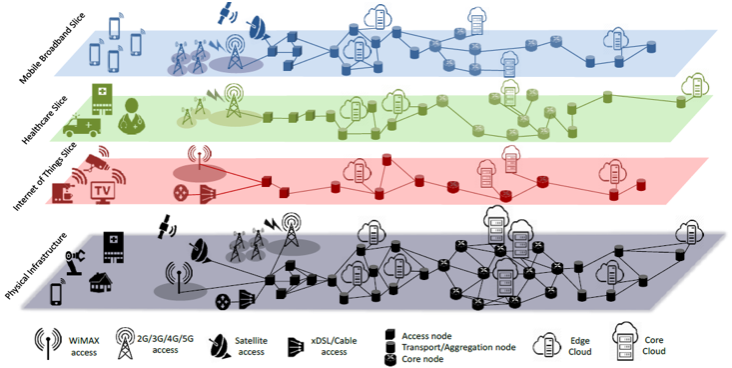
\includegraphics[width=.9\textwidth]{templates/images/chapter02/nw-slices.png}
    \caption{Network Slices on a Common Underlying Network. Source: \cite{OrdonezLucena2017NetworkSF}}
    \label{fig:nw-slices}
\end{figure}

The possibility to create on demand and in a programmable fashion, cost-efficient E2E network slices and dedicate them for the dynamic provisioning of diverse services is seen as a vital feature of 5G. In this vein, efforts are ongoing towards developing a 5G mobile system capable of deploying network slices of varying forms and sizes. Network slicing builds on top of the following seven main principles that shape the concept and related operations \cite{8320765}:

\begin{itemize}
    \item Automation: enables an on-demand configuration of network slicing without the need of fixed contractual agreements and manual intervention. 
    \item Isolation: is a fundamental property of network slicing that assures performance guarantees and security for each tenant even when different tenants use network slices for services with conflicting performance requirements.
    \item Customization: assures that the resources allocated to a particular tenant are efficiently utilized in order to meet the respective service requirements.
    \item Elasticity: is an essential feature related with the resources allocated to a particular network slice, in order to assure the desired \acrshort{sla} under varying resources and network conditions (e.g. the changes of network traffic or workload).
    \item Programmability: allows third parties to control the allocated slice resources (i.e. networking and cloud resources) via open \acrlong{api}s (APIs) that expose network capabilities facilitating on-demand service-oriented customization.
    \item End-to-end: is an inherent property of network slicing for facilitating a service delivery all the way from the service providers to the end-user. Such a property  stretches across different administrative domains and through that, unifies various network layers and heterogeneous technologies (e.g. \acrshort{ran}, core network, transport and cloud).
    \item Hierarchical abstraction: is a property of network slicing that has its roots on recursive virtualization, wherein the resource abstraction procedure is repeated on a hierarchical pattern with each successively higher level, offering a greater abstraction with a broader scope. In other words, the resources of a network slice, allocated to a particular tenant, can be further traded either partially or fully to yet another third  party. 
\end{itemize}

The network slicing process is broadly broken down into three main layers, namely the Service Instance layer, the \acrfull{nsi} layer, and the Resource layer. Each service instance reflects a service provided by a vertical segment, application provider or mobile network operator. The \acrshort{nsi} represents a set of resources customized to accommodate the performance requirements of a particular service and may contain none, one or a number of different sub-network instances. A sub-network instance can be a network function or a sub-set of network functions or resources realizing a part of an \acrshort{nsi}. 

\newpage

\acrshort{3gpp} refers to \acrlong{nssi} as \acrshort{nssi} and states that in order to be \acrshort{e2e}, an \acrshort{nsi} needs to consist of:

\begin{itemize}
    \item  \acrshort{nssi} \acrshort{ran}: an instance from a given (radio) access network slice subnet.
    
    A radio access network slice subnet consists of one or more \acrshort{ran} nodes (i.e. \acrshort{enb} nodes when using \acrshort{lte}, and \acrshort{gnb} nodes when using \acrshort{nr}), each embedding and delivering full radio access functionality to interact with the \acrshort{ue} over the radio interface. To introduce modularity and support for different deployment options, different initiatives has suggested the need to functionally split a \acrshort{ran} node into three types of units: \acrfull{ru}, \acrfull{du}, and \acrfull{cu}, briefly mentioned in Section \ref{chap:3gpp-rel15} as "\acrshort{ran} decomposition". For the most representative case, a \acrshort{ran} node may consist of a \acrshort{cu}, each serving one or more \acrshort{du}s, each in turn serving one or more \acrshort{ru}s.
   
    \item \acrshort{nssi} \acrfull{cn}: an instance from a given core network slice subnet. 
    
    A \acrshort{cn} slice subnet includes the functions from the \acrshort{3gpp} \acrshort{cn} that are in charge of providing connectivity between \acrshort{ran} nodes and the Data Network, as well as any other 3rd party \acrshort{af} providing value-added functionality.
    \item A Virtual Network providing connectivity within and across the two former \acrshort{nssi}s. 
    
    Focused on provided connectivity within the \acrshort{nsi} in an \acrshort{e2e} manner, the virtual network consists of a set of virtual links that may span across various network segments.
\end{itemize}

\acrshort{nssi}s resulting from the instantiation of the above-referred network slice subnets can be flexibly combined to provide different behaviors and performance levels, and hence different \acrshort{nsi}s.

%\newpage

\subsection{Roadmap of Network Slicing}
The implementation of network slicing needs to be gradual due to the evolution approach followed by the \acrshort{3gpp} 5G architecture in Rel. 15 and 16. Based on the network slicing roadmap proposed in \cite{4G_LTE_E2E-NS}, some of the most important phases expected are presented.

\begin{figure}[!ht]
    \centering
    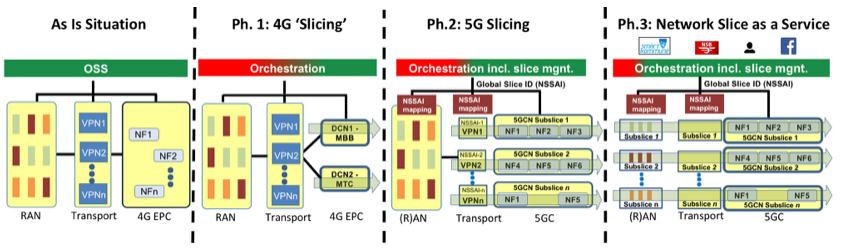
\includegraphics[width=.9\textwidth]{templates/images/chapter02/nw-slicing-roadmap.png}
    \caption{Roadmap of Network Slicing. Source: \cite{4G_LTE_E2E-NS}}
    \label{fig:nw-slicing-roadmap}
\end{figure}

"As-Is Situation" represents the current scenario where no network slicing and a single core network instance are present. In this scenario, \acrshort{qos} differentiation is offered at the Bearer level and \acrlong{apn}s (\acrshort{apn}s) are used for traffic separation while some form of isolation is implemented via a \acrfull{vpn}. Traffic can be separated for different customers but \acrshort{e2e} \acrfull{qos}, provisioning and the flexibility to have tailored network for vertical use cases cannot be implemented in an efficient manner.

Phase 1 is referred as  "4G Slicing" which  allows some level of traffic separation for overload mitigation and operational flexibility independent of other traffic.

Phase 2 will reference the specifications provided by the 3GPP Release 15 \acrfull{sa}, whose general concepts are outlined in Section \ref{chap:3gpp-rel15}. This phase is denominated as “5G Slicing” and consists of 5GCore. \acrshort{ran} and Transport layers support slicing via \acrfull{nssai}, with the latter leveraging \acrshort{vpn}s, each mapped according to said \acrshort{nssai}. Orchestration includes slice management but is not fully automated.

Phase 3 is labelled "\acrlong{nsaas}" (\acrshort{nsaas}) and is characterised by a fully automated network slicing operation. Unlike Phase 1 and 2 in which \acrshort{ran} and transport are not sliced, this phase involves slicing of the \acrshort{ran} and TN. In addition, it is expected to be able to host 3rd party \acrshort{nf}s, which enables new business opportunities.


\section{Network Slicing Types}

The \acrfull{itu} \cite{m.2083-0-201509} and \acrfull{5gppp} \cite{view_5g_architecture} have identified three broad use case families: enhanced mobile broadband, massive machine-type communications, and critical communications. Differences between these use cases amount to a set of heterogeneous and often contradictory requirements that cannot be satisfied by a one-size fits-all architecture. Diverse use cases need to be mapped to suitably tailored network structures. With this in mind, the architectural proposals for 5G aim to accommodate these use cases. The following sections describe how network slicing may utilise resources in order to serve these main use cases, while simultaneously respecting their requirements.

    \subsection{\acrfull{embb}}
    
    \acrshort{embb} is a set of services characterized by their need for high capacity links. This service type aims at supporting performance requirements of high data rates and high traffic densities. It is expected that the mobile capacity should increase 100 times over the capacity offered by current state of the art 4G systems to meet these requirements in urban user densities. Users should be able to achieve high speeds even at challenging scenarios such as on-the-go content streaming, while being at the cell edge and in crowded areas. In order to deliver NSaaS that provides this service, the \acrshort{csp} will place an emphasis on providing specific performance guarantees for \acrshort{kpi}s in the following areas: bandwidth, throughput, coverage and stability of connection.
    
    Some \acrshort{embb} services/applications will put more stress on the network from a \acrfull{up} traffic capacity point of view than others and thereby are more interesting from a Packet Core capacity perspective. This mandates specifying characteristics based on the need of each \acrshort{embb} service, Table \ref{tab:embb-sc-per} \cite{3GPP_TS_22.261} describes the performance requirements for high data rate and traffic density scenarios defined by 3GPP SA1 \cite{rel-15}.
    Depending upon the transmission delay, there is consideration on distributing User Plane on the Access Layer while hosting the rest of the functions centrally.

    \begin{sidewaystable*}
    \begin{threeparttable}
    \scriptsize
        \caption{\acrshort{embb} Scenarios and Requirements Identified by 3GPP}
        \label{tab:embb-sc-per}
    \begin{tabularx}{\textwidth}{@{}l*{10}{C}c@{}}
    \addlinespace
    %\addlinespace
    \toprule
        \multirow{2}{*}{Scenario} & \multicolumn{2}{c}{Experienced data rate} & \multicolumn{2}{c}{Area traffic capacity} & \multirow{2}{*}{User density} & \multirow{2}{*}{Activity factor} & \multirow{2}{*}{UE speed} & \multirow{2}{*}{Coverage} \\ 
        \cmidrule(r){2-3}\cmidrule(r){4-5}
        & Download & Upload & Download & Upload &  &  &  &  \\
    \addlinespace
    \midrule
    \addlinespace 
        Urban macro & 50 Mbps & 25 Mbps & 100 Gbps/km\textsuperscript{2} \tnote{4} & 50 Gbps/km\textsuperscript{2} \tnote{4} & 10 000/km\textsuperscript{2} & 20\% & Pedestrians and users in vehicles (up to 120 km/h & Full network \tnote{1} \\
        Rural macro & 50 Mbps & 25 Mbps & 1 Gbps/km\textsuperscript{2} \tnote{4} & 500 Gbps/km\textsuperscript{2} \tnote{4} & 100/km\textsuperscript{2} & 20\% & Pedestrians and users in vehicles (up to 120 km/h & Full network \tnote{1} \\
        Indoor hotspot & 1 Gbps & 500 Mbps & 15 Tbps/km\textsuperscript{2} & 2 Tbps/km\textsuperscript{2} & 250 000/km\textsuperscript{2} & \tnote{2} & Pedestrians & Office and residential \tnote{1} \tnote{3} \\
        Broadband access in a crowd & 25 Mbps & 50 Mbps & 3.75 Tbps/km\textsuperscript{2} & 7.5 Tbps/km\textsuperscript{2} & 500 000/km\textsuperscript{2} & 30\% & Pedestrians & Confined area \\
        Dense urban & 300 Mbps & 50 Mbps & 750 Gbps/km\textsuperscript{2} & 125 Gbps/km\textsuperscript{2} & 25 000/km\textsuperscript{2} & 10\% & Pedestrians and users in vehicles (up to 60 km/h) & Downtown \tnote{1} \\
        Broadcast-like services & Maximum 200 Mbps (per TV channel) & N/A & N/A & N/A & [15] TV channels of [20 Mbps] on one carrier & N/A & Pedestrians and users in vehicles (up to 500 km/h) & Full network \tnote{1} \\
        High-speed train & 50 Mbps & 25 Mbps & 15 Gbps/train & 7.5 Gbps/train & 1 000/train & 30\% & Users in trains (up to 500 km/h) & Along railways \tnote{1} \\
    \addlinespace 
    \midrule
    \end{tabularx}
    \begin{tablenotes}
        \RaggedRight
        \item[1] For users in vehicles, the UE can be connected to the network directly, or via an on-board moving base station.
        \item[2] A certain traffic mix is assumed; only some users use services that require the highest data rates [2].
        \item[3] For interactive audio and video services, for example, virtual meetings, the required two-way end-to-end latency (UL and DL) is 24 ms while the corresponding experienced data rate needs to be up to 8K 3D video [300 Mbps] in uplink and downlink.
        \item[4] These values are derived based on overall user density. Detailed information can be found in [10].
    \end{tablenotes}

    \end{threeparttable}
    \end{sidewaystable*}

    \subsection{\acrfull{urllc}}
    
    \acrshort{urllc} is a set of services with strict latency and reliability requirements. Basically, this service type aims at supporting performance requirements of low-latency and high-reliability while maintaining availability. Reliability increase can be achieved by dedicating appropriate resources to signalling, higher redundancy encoding and retransmissions. The above results in increased latency, proportional to packet size. If bandwidth requirements are low, by reducing packet size, low latency and high reliability simultaneously can be achieved, while reducing transmission times. 
    
    In order to guarantee the service is delivered at the required performance target, the \acrshort{csp} needs to prioritise resources to the \acrshort{urllc} slice, especially for mission-critical applications. It also needs to dynamically scale slices in the case of possible service degradation and may achieve high reliability by redundant transmission in the User Plane. 
    \acrshort{urllc} slices will provided by \acrshort{csp} for real-time control and feedback for the customer.
    
    From a communications perspective, two factors are of upmost importance and shall impact the definition of \acrshort{urllc} slice architecture in each Facility Site:
    
    \begin{enumerate}
        \item Latency: Sub-10ms \acrshort{e2e} latency is required for all use cases that can be mapped to the \acrshort{urllc} network slice. Note that many of the applications would require even sub-5ms latency, as seen on Table \ref{tab:urllc-sc-per}. 
        \item Reliability: The reliability is specified by the failure probability of packets (packet error rate) which are not successfully delivered to the receiver within the latency bound, as they are either erroneous, lost or arrive too late.
    \end{enumerate}
        
    \begin{sidewaystable*}
    \begin{threeparttable}
    \scriptsize
        \caption{\acrshort{urllc} Scenarios and Performance Identified by 3GPP}
        \label{tab:urllc-sc-per}
    \begin{tabularx}{\textwidth}{@{}l*{10}{C}c@{}}
    \addlinespace
    %\addlinespace
    \toprule
        Scenario & Max. allowed latency\tnote{2} & Survival time & Service availability\tnote{3} & Reliability\tnote{3} & User experienced data rate & Payload size\tnote{4} & Traffic density\tnote{5} & Connection density\tnote{6} & Service Area dimension\tnote{7} \\
    \addlinespace
    \midrule
    \addlinespace 
        Discrete automation & 10 ms & 0 ms & 99.99\% & 99.99\% & 10 Mbps & Small to big & 1 Tbps/km\textsuperscript{2} & 100 000 km\textsuperscript{2} & 1000 x 1000 x 30 m \\
        Process automation - remote control & 60 ms & 100 ms & 99.9999\% & 99.9999\% & 1 to 100 Mbps & Small to big & 100 Gbps/km\textsuperscript{2} & 1 000/km\textsuperscript{2} & 300 x 300 x 50 m \\
        Process automation - monitoring & 40 ms & 100 ms & 99.9\% & 99.9\% & 1 Mbps & Small & 10 Gbps/km\textsuperscript{2} & 10 000/km\textsuperscript{2} & 300 x 300 x 50 m \\
        Electricity distribution - medium voltage & 40 ms & 25 ms & 99.9\% & 99.9\% & 10 Mbps & Small to big & 10 Gbps/km\textsuperscript{2} & 1 000/km\textsuperscript{2} & 100 km along power line \\
        Electricity distribution - high voltage & 5 ms & 10 ms & 99.9999\% & 99.9999\% & 10 Mbps & Small & 100 Gbps/km\textsuperscript{2} & 1 000/km\textsuperscript{2} & 200 km along power line \\
        Intelligent transport systems & 30 ms & 100 ms & 99.9999\% & 99.9999\% & 10 Mbps & Small to big & 10 Gbps/km\textsuperscript{2} & 1 000/km\textsuperscript{2} & 2 km along road \\
    \addlinespace 
    \midrule
    \end{tabularx}
    \begin{tablenotes}
        \RaggedRight
        \item[1] Currently realised via wired communication lines. 
        \item[2] This is the maximum end-to-end latency allowed for the 5G system to deliver the service in the case the end-to-end latency is completely allocated to the 5G system from the UE to the Interface to Data Network.
        \item[3] Communication service availability relates to the service interfaces, and reliability relates to a given system entity. One or more retransmissions of network layer packets may take place in order to satisfy the reliability requirement.
        \item[4] Small: payload typically (<=) 256 bytes.
        \item[5] Based on the assumption that all connected applications within the service volume require the user experienced data rate.
        \item[6]  Under the assumption of 100\% 5G penetration.
        \item[7] Estimates of maximum dimensions; the last figure is the vertical dimension.
        \item[8] In dense urban areas.
        \item[9] All the values in this table are example values and not strict requirements. Deployment configurations should be taken into account when considering service offerings that meet the targets.
    \end{tablenotes}

    \end{threeparttable}
    \end{sidewaystable*}

\newpage
    
    \subsection{\acrfull{miot}}
    Heterogeneous access allows \acrshort{iot} devices to connect using whatever radio or fixed connectivity is available from both the device and the network. 5G-\acrshort{nr} utilizes spectrum bands for both low and very high bandwidth, as well as co-existence with cellular and non-cellular access networks but also other un-licensed radios. The operator is thus required to create and maintain the various instantiated \acrshort{iot} slices to offer services and enable the following scenarios:
    
    \begin{itemize}
        \item Enable individual needs of an \acrshort{iot} slice in terms of bandwidth, latency.
        \item Distribute efficiently resources of network slices involving resources at the Edge. Operators can offer resources and services at the edge of the network for \acrshort{iot} vendors to deploy (virtualised) applications and store collected data.
        \item Enable \acrshort{iot} Vendors to become “virtual operators” and build their own virtual network on top of a mobile operator and manage resources and services across a 5G network.
    \end{itemize}
    %added
    The \acrshort{miot} service type aims at supporting performance requirements of large number and high density of \acrshort{iot} devices. Some key aspects of these devices are their fully automated nature and the minimal interaction with humans, sending small amounts of information to the cloud. Some of these \acrshort{iot} devices are expected to be installed in remote, hard to access locations with bad coverage. Thus, a key requirement is the ability to use of very robust modulation and coding schemes. Median battery life is around a decade and the overall device cost should be low. Finally, their number is expected to explode in the coming years, thus base stations should be able to handle the additional overhead in signalling. In order to deliver NSaaS that provides this service, the \acrshort{csp} will place an emphasis on providing specific performance guarantees for \acrshort{kpi}s such as connection density (1,000,000 devices per km\textsuperscript{2}) and coverage (95\%) [55] while also guaranteeing security of the slice. Consumer privacy and security of the information proves of extreme importance for this type of service. 
    %eddad

\section{Network Slicing Requirements}
E2E network slicing inevitably adds an additional degree of complexity in the ecosystem, where each operator needs to deploy network slices internally and also facilitate the E2E deployment across several facility sites. Following there is a list of initial network slice requirements to be considered:

\begin{itemize}
    \item Orchestration: Slice-based services will require, not only the deployment across several administrative and operational domains, but also the integration of different technology domains. Their E2E nature requires orchestration of different computing and transport technologies.
    \item Operation: Each slice must behave as a dedicated network while sharing underlying resources, physical and virtual. Mechanisms need to be defined in order to abstract each customer slice.
    \item Scalability: The application of different \acrlong{sla} (SLAs) on the offered capabilities of management, control and customization of slices will directly impact scalability. Different levels depend on whether a network slice is inter or an intra-site.
    \item Service layer: The interaction with the vertical customers has an important requirement in the definition of the proper abstraction and templates to have a consistent service portfolio supported by different slice classes.
    \item Security and Isolation: Different network slices will be sharing the same infrastructure. The main requirement from the  \acrfull{iaas} and \acrfull{paas} is logical isolation of slices via appropriate networking, security grouping and multi tenancy implementation.
\end{itemize}

\newpage

\subsection{Network Slicing Use Cases}
    5G systems will support a wide range of use cases to vertical industries and their applications that wish to take advantage of their capabilities. These use cases will be supported by communication service providers (CSPs) who may offer \acrfull{nsaas} as a means of delivery. \acrshort{nsaas} is where the \acrshort{csp} offers network slices to their customers directly, rather than simply using slicing as an underlying capability to support other communication services. Each \acrshort{nsaas} will have a service description and \acrshort{sla} which will define the nature of the interaction between the \acrshort{csp} and said consumer.
    Slice providers and consumers can be described in terms of the business models between them and may fall into one of the following four categories:
    \begin{itemize}
    \item B2B (Business to Business): in which the \acrshort{csp} provides service to another business entity.
    \item B2C (Business to Consumer): in which the \acrshort{csp} providers service to an individual user.
    \item B2H (Business to household): in which the \acrshort{csp} provides service to a collection of individual users who form a single household and thus have some common characteristics.
    \item B2B2X (Business to Business to Everything): in which the \acrshort{csp} provides service to other business (such as other CSPs) who then offer a further service to their customers. 
    \end{itemize}
    From an architecture perspective, these four business models utilise one of two arrangements for the way in which the provider integrates their capabilities in order to deliver the end service.

\newpage

\section{Isolation on Network Slicing}
The use of a single, shared multi-domain network infrastructure makes isolation a key requirement in supporting network slicing. Isolation across \acrshort{nsi}s ensures that congestion, failures, attacks and lifecycle-related events (e.g. scaling in/out) of one \acrshort{nsi} does not negatively impact other \acrshort{nsi}s. Isolation is a broad concept embracing many dimensions, and will be studied from three main perspectives: performance, management and security. 

As previously mentioned, 5G network infrastructure is built out of a set of radio, computing, storage, and connectivity resources that can be flexibly combined to set up different \acrshort{nsi}s. These resources can be arranged into three main resource domains:

\begin{itemize}
    \item Radio Resource domain: consists of one or more antennas hosting RU functionality. A given antenna handles the operation of one or more cells, each assigned with specific radio resources to serve the \acrshort{ue} that are within the coverage area. These radio resources include multiple \acrfull{rf} carriers distributed across one or more spectrum bands which are consisted of several sub-carriers arranged into time-frequency resource grids known as \acrfull{prb}.
    \item \acrfull{dc} domain: consists of all the computing, storage, and networking resources that are defined within a \acrshort{dc}. Some are bundled together in physical, purpose-built devices ready to host \acrshort{pnf} instances, while others can be logically partitioned with the help of an abstraction layer. It is possible to have geographically distributed hierarchies, including edge and central \acrshort{dc}s. 
    \item \acrfull{tn} resource domain: consists of multiple physical \acrshort{tn} links providing connectivity throughout the entire hierarchical network infrastructure. These links can be similarly abstracted and partitioned, resulting in virtual links. Some of the \acrshort{tn} links will be defined within each administrative domain, providing connectivity between \acrshort{ran} nodes and \acrshort{dc}s, while others span across different domains, connecting central \acrshort{dc}s from different Facility Sites.
\end{itemize}

The resource (i.e. Radio, \acrshort{dc} and \acrshort{tn}) and management domains (i.e. 5G-\acrshort{ran} Controller, 5G-Core Controller, Transport controller, \acrshort{nfv}-\acrshort{mano}, and the \acrshort{e2e} Services Operations and Management) present the impact the three isolation dimensions have, without considering the presence of administrative domains. This means that the resource and management domains could be from the same or different sites.

    \subsubsection{Isolation in terms of Performance} 
    \label{chap:isolation-performance}
    
    Performance isolation in the network slicing context means that service-specific performance requirements are always satisfied on each \acrshort{nsi}, regardless of the congestions and workloads of other \acrshort{nsi}s running parallel. The level of performance committed for a \acrshort{nsi} needs to be assured in an \acrshort{e2e} manner (i.e. from the UE to the data center where the last \acrshort{nsi} component is allocated), across all the \acrshort{nssi}s that take part in the \acrshort{nsi}, including the connectivity between them. 
    \begin{enumerate}
        \item{Radio Resource Domain}
        
        Different \acrshort{nssi}s may share the limited set of radio resources available, mandating the definition of isolation mechanisms if performance isolation is desirable among \acrshort{nsi}s. This sharing is motivated by the fact that \acrshort{nssi}s are served within the same coverage area of a given antenna, and hence need to make a shared usage of the radio resources operated by this antenna. The isolation mechanisms vary depending on the scenario considered and include traffic isolation (i.e. avoid situations when traffic overload in one \acrshort{nssi} negatively affects the behavior of the rest of \acrshort{nssi}s) and electrical isolation (i.e. avoid mutual interference at the radio interface between the transmissions of different \acrshort{nssi}s) \cite{7891795}].
        Spectrum planning is the one that has the highest level of maturity, and hence can be seen as a feasible solution to be adopted for \acrshort{3gpp}'s Network Slicing Architecture.

\newpage

        \item{Datacenter Resource Domain} 
        
        \acrshort{dc}s include physical hardware that can be used to accommodate the \acrshort{nf}s of the different \acrshort{nsi}s. These \acrshort{nf}s can be either from the access part (\acrshort{an} \acrshort{nssi}s), or from the core part (CN \acrshort{nssi}s). The physical hardware of a \acrshort{dc} include both commodity and purpose-built hardware, while the latter can be seen as \acrshort{pnf} instances. Virtual resources result from the abstraction of the underlying commodity hardware, including computing, storage, and network equipment. The fact that \acrshort{vdu}s run on a common substrate brings potential risks on performance isolation, as failure or workload increase in one \acrshort{vdu} may decrease the performance of the rest of \acrshort{vdu}s sharing the same substrate. In virtualized environments, two approaches can be followed for \acrshort{vdu} hosting instantiation: 
        
        \begin{itemize}
        \item \acrshort{vnf} Instances from Different \acrshort{nsi}s on Separate Hardware Nodes.
        
        The first approach provides the most isolated environments for \acrshort{vdu} execution, as performance decrease and hardware failures in one node only affect the \acrshort{vdu} this node accommodates and not the rest of \acrshort{vdu}s. For the most critical \acrshort{nsi}s, compute nodes can be located in a dedicated availability zone, separated from any other zones in the \acrshort{dc}. Although allocating \acrshort{vdu}s from different \acrshort{nsi}s in different hardware nodes means achieving very great level of isolation among them, this approach commands high resource and energy usage.
        
        \item \acrshort{vnf} Instances from Different \acrshort{nsi}s Executed on a Shared Compute Node.
        
        The second approach allows for a more effective resource usage and energy efficiency, at the cost of providing less isolated environments for \acrshort{vdu} execution. Unlike the first approach, hardware failures and decreases of performance in one node may affect all the \acrshort{vdu}s running on this node.
        \end{itemize}

\newpage

        The introduction of server virtualization allows definition of \acrshort{vdu}s on top of the same compute node, providing them with separated execution environments. The isolation that each execution environment provides depends on the type of virtualization technology used. Currently, four types of virtualization technologies are available, each with different implications on the security ring-model as depicted in Figure \ref{fig:comparison-virtualization}. 
        
        \begin{figure}[!ht]
            \centering
            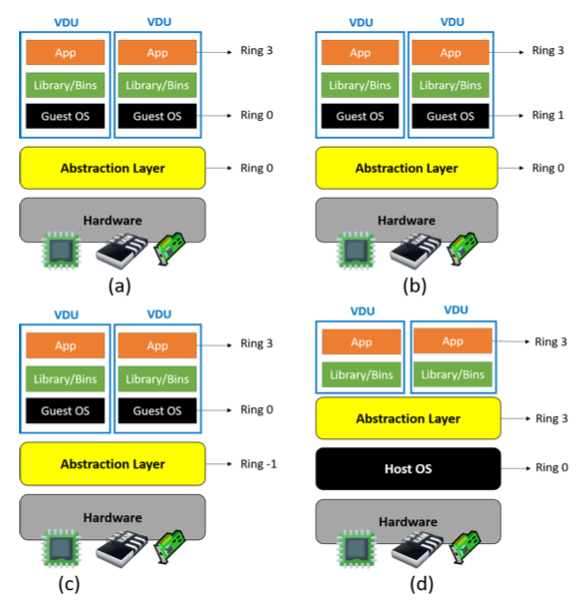
\includegraphics[width=0.75\textwidth]{templates/images/chapter02/comparison-virtualization.png}
            \caption[Comparison of Server Virtualization Technologies]{: (a) Para Virtualization, (b) Full Virtualization, (c) Full Virtualization with Hardware Assist\protect\footnotemark and (d) \acrshort{os} Virtualization. Source: \cite{adrian_gallego_2019_2668763}}
            \label{fig:comparison-virtualization}
        \end{figure}

\footnotetext{Note that full virtualization technologies with hardware assist (i.e. Intel VT and AMD-V) introduces a more privileged ring level (ring -1) to the original x86 ring model. In this new ring level, the abstraction layer uses processor extension to intercept and emulate privilege instructions, leaving ring 0 available for \acrshort{vdu}s, whereas this would be reserved by the operating system's kernel.}

        As result of the application of the four above-referred technologies, two types of \acrshort{vdu}s are outlined: \acrshort{vdu}s with their own guest \acrshort{os} and \acrshort{vdu}s sharing the same host \acrshort{os} as depicted in Figure \ref{fig:vm-unikernel-container}. 
        
        Those result in two types of abstraction layer being identified:
        \begin{itemize}
            \item Hypervisor: applicable to para virtualization, full virtualization, and full virtualization with hardware assist. This abstraction layer allows the definition of \acrshort{vdu}s, each with its guest \acrshort{os}. The \acrshort{vdu}s resulting from the hypervisor are traditional \acrlong{vm}s (VMs). However, in recent years, a new type of \acrshort{vdu}, named "unikernel", resembles a \acrshort{vm} but is built with a lightweight and specialized guest \acrshort{os}. Unlike \acrshort{vm}s, a unikernel can only run a single process, and cannot benefit from full virtualization with hardware assist, as it contains only aboslutely necessary components to run a specific application.
            \item Container engine: applicable to \acrshort{os} virtualization, this abstraction layer allows the definition of \acrshort{vdu}s running on top of the same \acrshort{os}, without the possibility to host their own. These \acrshort{vdu}s resulting from the abstraction carried out by container engine are referred to as containers.
        \end{itemize}

        \begin{figure}[!ht]
            \centering
            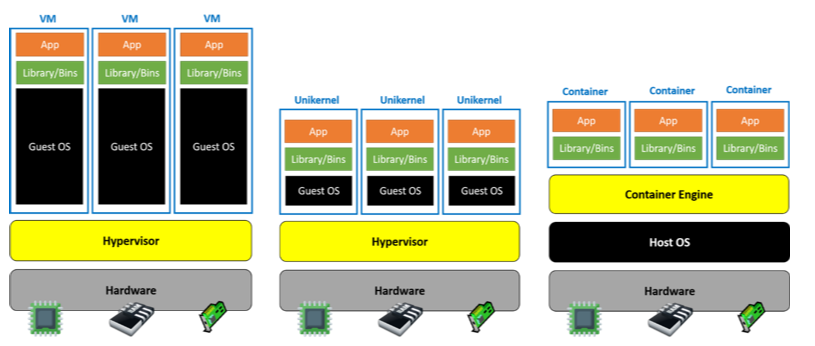
\includegraphics[width=.9\textwidth]{templates/images/chapter02/vm-unikernel-container.png}
            \caption{\acrshort{vm}s vs Unikernels vs Containers in Terms of Isolation. Source: \cite{adrian_gallego_2019_2668763}}
            \label{fig:vm-unikernel-container}
        \end{figure}
        
        \begin{table}[!ht]
           \begin{threeparttable}
        \caption[Comparison Between Types of \acrshort{vdu}s]{on Top of which \acrshort{vnf} Instances Run}
        \label{tab:vdus}
        \setlength\tabcolsep{1pt} % make LaTeX figure out intercolumn spacing
        
        \begin{tabular*}{\columnwidth}{@{\extracolsep{\fill}} lllll}
        \toprule
             \acrshort{vdu} Type &Ring Level &Isolation provider &Image size &Operation agility \\
        %     \multicolumn{4}{c}{Accuracy (\%)} \\ 
        %\cmidrule{3-6}
        %     & & K3 & K6 & L1 & mean\tnote{c} \\
        \midrule
              \textbf{\acrshort{vm}} &Level 0 or -1 &Hypervisor &Large &Low \\
        \addlinespace
             \textbf{Unikernel} &Level 0 &Hypervisor & Small & Medium \\
        \addlinespace
              \textbf{Container} &Level 3 enforced at Level 0 &Host \acrshort{os} &Medium &High\\
        \bottomrule
        \end{tabular*}
        
        \smallskip
        \scriptsize
           \end{threeparttable}
        \end{table}
        
        As seen from Table 5.2, the most isolated environment is provided with a \acrshort{vm} at the cost of less speed of operation, followed by the unikernel that provides more agility and reduced image size. Containers provided the least degree of isolation, although they allow for great agility in run-time operations. The selection of each \acrshort{vdu} type for \acrshort{vnf} hosting depends on the necessity of the \acrshort{vnf} operation, and the degree of isolation required. The use of separate physical appliances and \acrshort{vm}s are known to be matured solutions for providing isolation in the \acrshort{dc} resource domain. Unikernels, although bringing some benefits compared to \acrshort{vm}s, need to reach more maturity and popularity before considering them as firm candidates to replace \acrshort{vm}s. Finally, containerization technology is gaining some maturity in the last years, empowered by the adoption of Service Based Architecture (SBA) for \acrshort{3gpp}’s 5GC. The adoption of this solution is expected for \acrshort{3gpp} Rel. 15 and 16 SA.

        \item{\acrfull{tn} Resource Domain}
        
        Virtual links resulting from the abstraction of the underlying \acrshort{tn} links can be arranged into virtual networks, each providing intra-\acrshort{nsi} connectivity (i.e. connectivity across P/\acrshort{vnf} instances from the \acrshort{nssi} \acrshort{ran} and \acrshort{nssi} CN) with performance guarantee. Both wired and wireless \acrshort{tn} technologies can be used, with the former including optical and gray optics, whereas the latter encompasses both wireless (i.e. packet microwave and mm-wave) and satellite solutions as Physical Layer (L1) technologies. 
        It is to be expected that, in some cases, the common \acrshort{tn} infrastructure will be shared between multiple 5G services. Network slicing isolation is thereby achieved by the introduction of some form of encapsulation, for the differentiation of virtual links operating on top of a shared substrate and the selection of corresponding Layer technologies towards the realization of these virtual networks. The introduction of encapsulation enables different virtual networks to be deployed on top of physical links that compose the underlying \acrshort{tn} infrastructure, differentiated by the degree of isolation they provide.
        
        Soft isolation is implemented by statistically multiplexing the traffic from two or more VNs onto a common circuit switched connection using a packet technology (e.g., Ethernet \acrfull{vlan}, \acrfull{mpls} tunnel). Isolation is enforced at the packet layer, permitting sharing of resources across different virtual links, since resources are only dedicated on a temporary basis. This allows greater statistical multiplexing on network resources in different links and leads to better economy at the cost of opening up the possibility to suffer from congestion in the network, in all the virtual links making use of those resources.
        
        Hard isolation is implemented by providing independent circuit switched connections for the exclusive use of one VN (e.g. Time Division Multiplexing (TDM) based approaches, assignment of different fibre cables etc.). Hard isolation solutions allow reaching high degree of isolation between virtual links, at the expense of allocating dedicated resources on a long term and end-to-end basis. This means that that the full cost of the resources must be borne by the \acrshort{nsi} whose VL is allocated with those resources.   
\end{enumerate}
    
    \subsubsection{Isolation in terms of Management and Orchestration}
    \label{chap:isolation-mano}
    Isolation at the \acrshort{mano} level assumes the existence of tenants at the orchestration level (e.g., Multitenancy in \acrshort{osm}, ONAP). Each tenant has an exclusive view and management of specific \acrshort{vnf}s, NSs and the isolated resources at the \acrshort{ran}, Core and TN, enabling the management and orchestration of a particular slice. A default master tenant usually called “administrator”, is in charge of the management and orchestration of all slices and the physical and logical resources that comprise them.  Multitenancy at the \acrshort{vim} level articulates the isolation mechanisms defined in compute, storage and tenant networks, allowing for a tenant to only see and administrate the resources that are assigned to it.
    One important concept is the shared part. It is important to employ the isolation mechanisms mentioned in previous sections (e.g. \acrshort{ran} slicing at the carrier and \acrshort{prb} level, transport slicing at the wavelength, time slot, logical bandwidth level). From previous sections, it is apparent that shared resources is a critical part of operation. As to be expected, isolation cannot be guaranteed in all cases (i.e. when sharing same antenna, cable and compute node across multiple slices). Tenants may demand isolation of resources allocated to management regarding isolation of compute and storage resources. This makes it possible to obtain all properties of virtualized computing systems, as mentioned in the previous section, enabling tenants with different levels of isolation at the management level.

    \subsubsection{Isolation in terms of Security}
    \label{chap:isolation-security}
    Security as a term, encompasses different aspects in the provisioning, operation and use of any network services. For that reason, slices must adhere to general security properties, based on the three dimensions of a network service. These dimensions have obvious implications to slice isolation and namely are:
    
    \begin{itemize}
        \item Protection: in what implies that a service is immune to attacks from any adversary attempting to distort in any means its functionality or features. Isolation in terms of protection ensures each slice is immune from attacks on other slices or parts of the external network.
        
        \item Privacy: requiring that no data from any actor in the service (provider, consumer, end user) is accessed by unauthorized parties. Isolation in terms of privacy ensures each slice has adequate mechanisms to protect integrity and confidentiality and sensitive information (i.e. configuration, management, subscriber, and accounting information) from being accessed by other entities.
        
        \item Accountability: which translates into enforcing proper authentication, authorization and accounting, so no action is performed without verifying the identity, access rights and properly maintaining a record for further auditing.
    \end{itemize}


\chapter{5G Verticals Innovation Infrastructure}
%% This is an example first chapter.  You should put chapter/appendix that you
%% write into a separate file, and add a line \include{yourfilename} to
%% main.tex, where `yourfilename.tex' is the name of the chapter/appendix file.
%% You can process specific files by typing their names in at the
%% \files=
%% prompt when you run the file main.tex through LaTeX.
The 5G-VINNI concept is to develop an E2E 5G facility that can be used to primarily demonstrate the practical implementation of infrastructure to support the key 5G KPIs and to accelerate the uptake of 5G in Europe by lowering the entry barrier for vertical industries to pilot use cases dependent upon those KPIs. However, 5G-VINNI is not intended to be simply a group of interconnected test facility sites as seen on Figure \ref{fig:5g-vinnimap} \cite{5gvinni-site-map} – it is underpinned by principles that will allow for highly dynamic and flexible network architectures, service deployment and testing, that will create new technical and commercial service deployment models. These will in turn drive inter-facility interconnection to enable virtualized functions from the network and service layer to be called upon from any facility, with complete location agnosticism – a truly cloud-based network instantiation that has no functional boundaries, implemented across multiple facility sites.



\newpage

\section{Architectural Principles}
\acrshort{5gvinni} is underpinned by key architectural principles identified in the \acrshort{5gvinni} proposal document. These are:
\begin{itemize}
    \item Common and consistent sets of capabilities. 
    
    All \acrshort{5gvinni} facility sites support a core set of functional components and capabilities, meaning that partners that perform trials can be assured a baseline set of capabilities at any facility.
    
    \item     Interworking between facility sites. 
    
    A key strength is the ability to perform \acrshort{e2e} testing between sites. This mandates a common set of interfaces to be supported by all facility sites to allow interaction between control plane systems and the flow of traffic.
\end{itemize}

\begin{figure}[!ht]
    \centering
    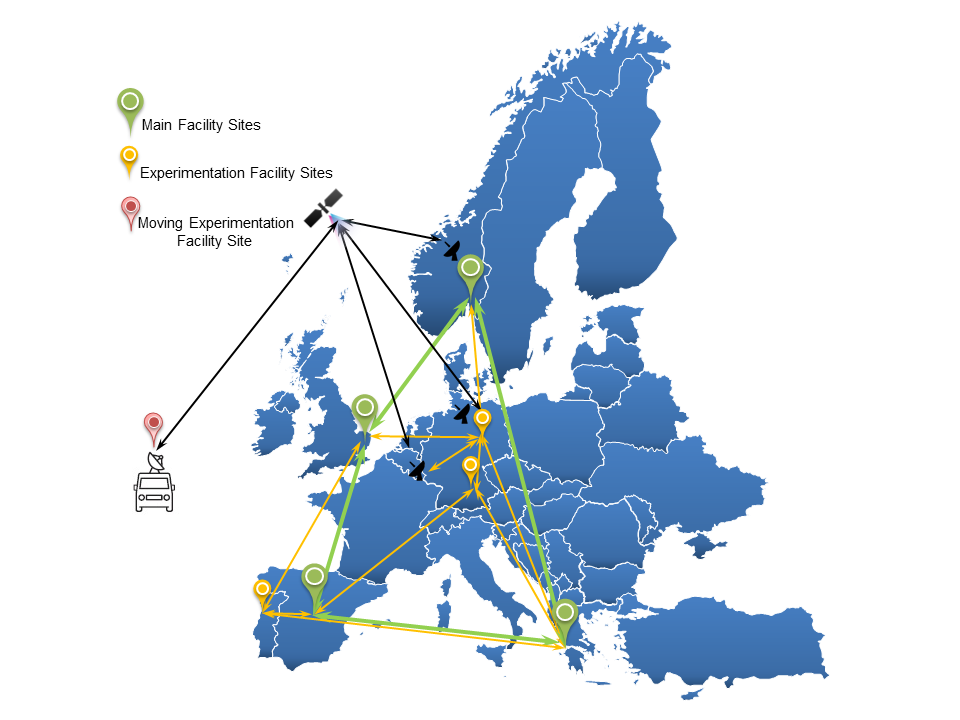
\includegraphics[width=.9\textwidth]{templates/images/chapter03/5g-vinnimap.png}
    \caption{5G-VINNI Facility with Main and Experimentation Sites. Source: \cite{5gvinni-site-map}}
    \label{fig:5g-vinnimap}
\end{figure}

\newpage
\begin{itemize}
    \item     Optional elements to support specific use cases, testing and \acrshort{kpi}s. 
    
    In order to achieve this, additional functions may be supported at sites that require them, in order to meet proprietary requirements.
    
    \item     Support for Network Slicing. 
    A key component of \acrshort{5gvinni} is the support of network slicing. This is essential for each site in order to allow simultaneous testing of multiple use cases on common infrastructure.
    
    \item     Ability for each site to evolve during the project. 
    
    5G has an underlying principle of networks built using \acrshort{vnf}s. The iterative nature of functional capabilities permits quick and with frequency changes to the network. 5G specifications is currently a work in progress and so, within the timeline of the project, standards and state-of-the-art implementations will potentially shift significantly. Therefore it is fundamental that \acrshort{5gvinni} facility sites are designed in such a way so as to allow implementations to keep pace with technological evolutions. This will maintain the \acrshort{5gvinni} facility's relevance to vertical industry partners' testing requirements throughout the duration of the project.
    
    \item     Openness and accessibility of the framework. 
    
    The design of the each facility aims to allow the flexibility and accessibility for vertical industries to run and test novel pilot use cases.
\end{itemize}
With virtualisation, orchestration and network slicing all included as underpinning architectural principles and identified as the basis for implementation as early as \acrshort{5gvinni} Release 0, it is clear that a multi-layered implementation is expected with network management and orchestration as disciplines that are pivotal for the instigation of network functions and network slices within one or multiple facility sites.

\section{Template Facility Architecture}
In the lower layer is the infrastructure, \acrshort{vnf}s and \acrshort{pnf}s in the \acrshort{ran} and Core infrastructure for the transport domain, which are expanded upon on Sections \ref{chap:vinni-ran} and \ref{chap:vinni-core-transport-infrastructure} respectively. 
Above the Network Domains, \acrshort{nfv}-\acrshort{mano} focuses on virtualization-specific tasks (i.e. management at the virtualized resource level) while domain controllers operate on non-virtualization-related operations (i.e. management at the application level). This architecture can be implemented in a range of ways, which allows individual facility sites to realize a network that can deliver a set of \acrshort{kpi}s, whilst adhering to the principles of \acrshort{5gvinni} as a whole.

    \subsection{User Equipment}
    For the most part, end-user devices are outside of the scope of \acrshort{5gvinni} as devices tend to be tied to vertical use cases and as such are in the domain of prospective ICT-19 projects. It is clear that for a device to connect to a \acrshort{5gvinni} facility site’s infrastructure, it should support reciprocal interface requirements mandated upon the \acrshort{ran}. Where required, \acrshort{5gvinni} facility sites may support devices that are specific to use cases and hence need to meet specific requirements. Theses include (but are not limited to):
    
    \begin{itemize}
        \item \acrshort{lte}-M
        \item \acrfull{nbiot}
        \item \acrfull{fwa} 
        \item \acrfull{v2x}
        \item Experimental functionality for future capabilities (R16, R17 and beyond)
        \item Air interface and connectivity testing.
    \end{itemize}
    
    \subsection{\acrfull{ran}}
    \label{chap:vinni-ran}
    Initial \acrshort{5gvinni} \acrshort{ran} architecture is aligned with what is being planned for early launches of commercial 5G networks in Europe. This will create a 5G research environment that, in some ways, closely reflects functionality and performance offered by early commercial 5G networks. Some of the \acrshort{5gvinni} facility sites may implement \acrshort{sa} architecture from start while other facilities may align with the development related to early commercial networks then migrate from \acrshort{sa} architecture during the later Releases of the \acrshort{5gvinni} project. 
    
    The \acrshort{5gvinni} \acrshort{ran} will initially offer service opportunities in the 3.5 GHz frequency band (\acrshort{3gpp} n77/n78, referred to as "mid-band") and in subsequent phases also in the 26 GHz frequency band (\acrshort{3gpp} n258, referred to as "high-band"). Specific details of what will be supported at the different facility sites depends on \acrshort{nsa} or \acrshort{sa} implementation as well as spectrum availability and device capabilities. Most notable features that need to be supported are:
\newpage
        \begin{itemize}
        
        \item \acrshort{lte} – \acrshort{nr} Dual Connectivity
        
        Dual Connectivity (EN-DC) is a mandatory part of 5G \acrshort{nsa} operation that allows early introduction of 5G by overlaying \acrshort{nr} to existing \acrshort{lte} networks connecting to the 5G enabled \acrshort{cn}.
        
        \item Uplink/Downlink Decoupling
        
        \acrshort{5gvinni} \acrshort{nsa} architecture will support uplink/downlink decoupling allowing \acrshort{lte} spectrum (using lower frequency bands than \acrshort{nr}) with superior coverage to be used for uplink traffic while \acrshort{nr} spectrum with superior peak data rate and latency is used for downlink. 
        By combining the high speed and low latency of the \acrshort{nr} downlink with the larger coverage and high reliability of the \acrshort{lte} uplink, the coverage versatility provided by \acrshort{nr} spectrum is significantly extended. 
        
        \item \acrshort{lte} – \acrshort{nr} Aggregation
        
        Increases user peak bitrates and app coverage by combining one or more \acrshort{lte} carriers with one or more \acrshort{nr} carriers to allow users to experience higher speeds in the network.
        
        \item Multiple Input Multiple Output (MIMO) 
        
        Massive numbers of antenna elements is a key feature for \acrshort{nr} systems. Especially for high frequency bands, the introduction of multi-antenna arrays enables numerous benefits. Most notably, beamforming improves data transmission coverage and link performance, while interference is minimized further improving throughput for cell-edge users.
        
        \item Numerology support 
        
        3GPP \acrshort{tr} 38.912 \cite{3GPP_TR_38.912} \acrfull{scs} enables \acrshort{ran} systems to deliver lower latency compared to legacy commercial \acrshort{lte} networks.
\newpage
        \item \acrshort{nr} Carrier Bandwidth
        
        Mid and low frequency carrier bandwidth is naturally narrower than high frequency bands. As a result, up to 100 MHz carrier bandwidth can be supported for mid-band versus 50 to 100 MHz in high frequencies\footnote{Actual implementation needs to conform with spectrum availability at the different \acrshort{5gvinni} facility site regions.}.
        
        \item Modulation
        
        64 \acrfull{qam} in uplink and downlink shall be supported, with some experimental uses of 256QAM for downlink transmission. 
        
        \item Network slice aware \acrshort{ran}
        
        For \acrshort{ran}, a network slice provides additional information on the policy for handling traffic in addition to the regular \acrshort{qos} for radio bearers.
        
        \item \acrshort{ran} integration with \acrshort{nr} Standalone (\acrshort{sa}) Core architecture
        
        When \acrshort{5gvinni} facility sites implement \acrshort{sa} architecture, \acrshort{ran} functionality shall be adopted to fulfil applicable requirements. This requires that \acrshort{ran} and UE progression needs to be aligned with the introduction of 5G Core, as this introduces new interfaces and protocols.

        \item Dynamic spectrum sharing
        
        Radio access node will dynamically determine if an \acrshort{nr} or \acrshort{lte} user is to be served, allowing NR to use the same legacy frequency bands as LTE.

    \end{itemize}
    
    \subsection{Core and Transport Infrastructure}
    \label{chap:vinni-core-transport-infrastructure}
    As previously discussed, 5G System as defined in 3GPP Rel. 15 can be realized either by 5G-\acrshort{nr} RAN connected to \acrshort{epc} (\acrshort{nsa}) or 5G-\acrshort{nr} connected to 5G Core (\acrshort{sa}). While EPC is used in \acrshort{nsa} as an evolution of the current \acrshort{lte} Core network, 5G Core is a service-based architecture with new functional nodes. 

    Transport is the part of the network that comprises the intermediate links between the CN or backbone and the sub-networks at the "edge" of the hierarchical network. Backhaul plays a vital role in mobile networks by acting as the link between \acrshort{ran} and Core.

        \subsubsection{Wireless backhaul}
        Wireless technologies operating at microwave and millimetre-wave frequencies, allow operators freedom regarding base station and small cell wireless-based backhaul. 
        
        Packet microwave or mm-wave technologies are increasingly prevalent elements of Heterogeneous Networks (HetNets), offering ample IP capacity for backhaul. \acrfull{ptp} systems can also be used as relays in a multihop backhaul network. Various topologies can be used in a backhaul deployment, depending on each specific network’s need (e.g. point-to-point line, tree structure, mesh, ring or a combination). Reliability can be achieved by using redundancy in equipment and appropriate topologies.
        In \acrshort{5gvinni}, the wireless transport network can provide a versatile solution for backhaul as a fibre substitute, as well as transport for \acrshort{iot} applications. 
        
        \subsubsection{Optical Backhaul, Midhaul and Fronthaul}
        In \acrshort{5gvinni} an optical transport solution, can be used to support backhaul, midhaul and fronthaul alternatives. Different functions in the \acrshort{gnb} result in different demand for bandwidth and latency, thus requiring different transport alternatives.

       The mid and front-haul options are currently under development (outside the scope of \acrshort{5gvinni}) and are foreseen to be integrated in the facility infrastructure along the course of the project.

        \subsubsection{Satellite backhaul}
        \acrfull{mno} likely perceive satellite backhauling services as islands of costly, difficult to integrate and inflexible connectivity. However, with the significant recent advances in satellite technology (e.g., High-Throughput Satellite) satellites can deliver cost-effective high-performance solutions to unserved and underserved areas.
        
        \subsubsection{Backhaul connectivity}
        Any backhaul connectivity deployment includes an edge node and a central node connected using a backhaul link, seen as a transport layer for the messages between the edge and the central node.
        
        The UE connects to a local terrestrial access network which is represented in this case by a 5G \acrshort{gnb}. In order to assure the connectivity to the local terrestrial access network though the different backhauls, the 5G Core Network is deployed with a functional split between the edge and central nodes.
        One of the \acrshort{nf}s associated to the backhaul connectivity architecture is the edge router which acts as a \acrfull{sd-wan} router. Data traffic is then steered according to a set of routing policies over the available backhauls previously mentioned.
        
    \subsection{Management and Orchestration}
    Management and Orchestration is a key capability for provisioning network slices. Once the underlying programmable infrastructure has been established, there is a need for components that are able to manage and orchestrate the resources within and across domains \cite{view_5g_architecture}. These functions are:
    
        \subsubsection{\acrshort{nfv} \acrshort{mano}}
        From a resource management point of view, services are deployed and operated as \acrshort{nfv} NSs. With \acrshort{nfv} \acrshort{mano}, facility operators are able to deploy and execute services in the \acrshort{nfvi} with great agility and flexibility. The \acrshort{nfvi} in \acrshort{5gvinni} facility spans across the seven facility sites and consists of different PoPs for \acrshort{vnf} deployment and execution, ranging from cell sites to regional DCs. 
        Each facility site will have its own \acrshort{nfv} \acrshort{mano} stack to manage and orchestrate \acrshort{nfv} NSs within its administrative domain while exposing a set of SBIs and NBIs to facilitate the interaction with the rest of facility site components. 
        The stack deployed at each facility site has three types of functional blocks (NFVO, VNFM, and \acrshort{cim}) and four data repositories (NS Catalog, \acrshort{vnf} Catalog, \acrshort{nfv} Instances Repository, and \acrshort{nfvi} Resources Repository). This guarantees interoperability across \acrshort{5gvinni} facility sites at \acrshort{nfv} level, regardless of any implementation-specific issues. The fact that \acrshort{etsi} \acrshort{nfv} defines \acrshort{nfv} \acrshort{mano} stack as a reference framework not only allows network operators and vendors to implement its components using open source or vendor specific solutions but also introduce some architectural modifications.
        
        \subsubsection{Network-Domain Controllers}
        \begin{enumerate}
            \item \acrshort{ran} and Core Domain Controllers
            
            The Domain Controllers at the \acrshort{ran} and Core are in charge of managing the different \acrshort{nf}s at the application level (independently of their deployment), and in general to provide control on all the non-virtualization-related operations. Core \& \acrshort{ran} domain controllers can be mapped to the EMS function group of FCAPS (Fault, Configuration, Accounting, Performance and Security management) for the functional/application part of the underneath deployed \acrshort{pnf}s and \acrshort{vnf}s. In this way we can say that these domain controllers perform changes at the application level in a “vertical” way on functions “horizontally” deployed by the NFVO.
            
            \item Transport Domain Controllers
            
            The Domain Controllers at the transport include components such as SDN controllers or \acrshort{mpls} management and control components. In \acrshort{5gvinni} the Transport network will provide advanced backhaul functionality, to interconnect for instance different locations from a common site.
            \acrshort{mpls} networks for instance are well-known solutions used for several years in the transport network. \acrshort{mpls} allows the visualization of the \acrshort{e2e} path instead of a hop by hop vision.
            
            \begin{figure}[!ht]
                \centering
                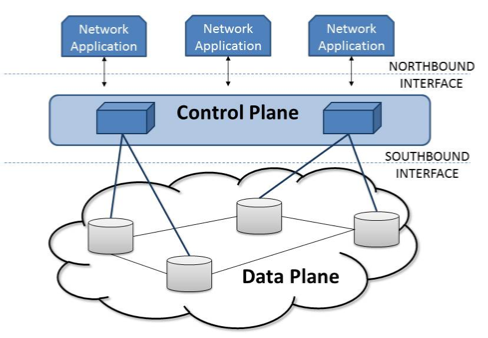
\includegraphics[width=.9\textwidth]{templates/images/chapter03/sdn-architecture.png}
                \caption{SDN Architecture According to IETF RFC 7426. Source: \cite{view_5g_architecture}}
                \label{fig:sdn-architecture}
            \end{figure}  
            
            The \acrshort{cp} and the data plane are separated from each other. In addition, the \acrshort{cp} is logically centralized in a software-based controller defined as the “network brain”, while the data plane is composed of network devices (“network arms”) that forward packets. The \acrshort{cp} includes both northbound and southbound interfaces. The northbound interface provides a network abstraction to network applications, and the southbound interface (e.g., OpenFlow) standardizes the information exchange between the control and data planes \cite{rfc7426}.
            
        \end{enumerate}

        \subsubsection{\acrshort{e2e} Service Operations and Management}
        \acrshort{e2e} Service Operation and Management, within the \acrshort{5gvinni} architecture, encompasses the management and operations of \acrshort{e2e} services that span multiple domains. It translates service design into configuration of resources (physical and virtualized) needed for service establishment. Using orchestration to coordinate between domain controllers and \acrshort{nfv}-\acrshort{mano}, \acrshort{e2e} services may span multiple network domains provided by different administrative entities (e.g., different network service providers or external partners).
        Effectively, \acrshort{e2e} \acrshort{mano} connects the business needs of verticals to the resource and network capabilities exposed by management and partner provider domains. It thereby enables orchestration and management across multiple domains, doing so by offering customer facing services northwards via standardised API’s to fulfil service requirements. The \acrshort{e2e} \acrshort{mano} translates business services into their corresponding component network services and requests the services from the appropriate domain. In this way the \acrshort{e2e} \acrshort{mano} abstracts how the business services are realised at the resource level, thereby allowing verticals to focus on their Service Level Agreements (SLAs) rather than the service implementation itself.

    \subsection{Security, Testing and Monitoring Architecture}
    With the use of \acrshort{nfv} and SDN in 5G, one of the main priorities is for a secure cloud environment between tenants and slice instances. Security needs to be present in all sub-domains of the cloud to address the current threat landscape with sophisticated actors, adhere to privacy and security regulations in the different markets and ensure isolations of tenants and network slices. The main security controls that need to be established in the cloud domain are:
    \begin{itemize}
    \item Infrastructure network zoning model that applies to all layers of the infrastructure.
    \item Solid multi-tenancy capabilities through the infrastructure platform.
    \item Security monitoring through flow based network analytics.
    \item Centralized logging with analytics capabilities.
    \item Server integrity checking and configuration auditing.
    \end{itemize}
    Note that there are other important security functions, such as DDoS protection, Intrusion Detection and Prevention Systems (IPS/IDS), antivirus, antimalware etc. The aim is not to cover all security requirements and features in this section. In the following, briefly described are architectural principles for the zoning model and multi tenancy.

        \subsubsection{Zone Model}
        The infrastructure network zoning model is fundamental in addressing the shared technology challenge in a multi-tenant platform. The defined zone model regulates how the cloud infrastructure is built and how segmentation is achieved.
        A security domain is an entity that defines the level of control and governance present; it does not itself have any policies, but exists to define where boundaries are present. A domain can consist of one or more security classes. Security domains defined in level of trust are: un-controlled, controlled, restricted, secure, and externally controlled domain with traffic not allowed to flow directly between non-adjacent domains. Security Zone Classes is a concept of aggregating network zones with the same exposure and security levels. Traffic from one security class to another will need to pass two different layers of security with one being logical or virtual and with the second layer being physical.

        \subsubsection{Multi-tenancy}
        Multi-tenancy enables separation between tenants running services in a shared environment. In a multi-tenant deployment, the resources controlled by one tenant are physically or logically separated and secured from other tenants. Multi-tenancy is a key requirement for services across both public and private cloud environments.

    The testing architecture has a purpose that is primarily establishing automation services that encompasses every phase of the infrastructure deployment. Nowadays, this is considered a very important stage given the number of performance and interoperability variables at stake in modern virtualized systems. The second purpose of the testing infrastructure is to provide testing and experimentation services to the vertical service operators but also to the mobile operators themselves for network maintenance purposes. This is a fundamental step for ensuring reliability, resilience, and performance of the slice components and of the slice as a whole during the slice deployment phase, a due process before handing the slice over to the customer. Such system is used to monitor all the components, from the virtualised infrastructure to the Quality of Experience (QoE) of the traffic carried by the network. While its presence would be highly suggested, the complexity of virtualized networks make a full monitoring extremely heavy and resource-demanding.

\section{Interconnection and Interoperability of sites}

    \subsubsection{Interconnection Between Sites}
    This section explains the architectural requirements in terms of connectivity between sites. As a main principle, it is important that all sites have IP connectivity with each other. For such purpose, each site shall have one or more facility site gateways (FSGW) that fulfils the following requirements. In the long term solution, two FSGWs can be preferred for increased load balancing and resilience capabilities. 
    
    \begin{itemize}
        \item Public IP.
        \item Routing protocols, especially exterior gateway protocols, such as Border Gateway Protocol (BGP).
        \item Generic Routing Encapsulation for the establishment of GRE Tunnels.
        \item Internet Protocol Security (IPsec) protocol suite.
    \end{itemize}
    For \acrshort{qos} Differentiation on the connection between sites the following options are under evaluation. 
    \begin{itemize}        
        \item Best Effort Internet\footnote{In the initial phase, all sites will use Best Effort internet. However, the possibility that the connection between some specific pair of sites will be upgraded gradually to \acrshort{mpls}-\acrshort{vpn} and/or \acrshort{sd-wan} with \acrshort{mpls} Core is under evaluation.}.
        \item \acrshort{sd-wan}, where the traffic can be sent over a combination best-effort Internet paths and some way of using \acrshort{mpls} Core or direct DiffServ-enabled traffic exchange between the operator domains.
    \end{itemize}
    
    This will enable SD-WAN for \acrfull{asq} interconnection paths between sites and value added connectivity (VAC) triggered and handled on-demand for end-point traffic flows whose traffic can be steered. For the support of use cases and scenarios beyond the basic service offerings (based on best-effort Internet interconnection) the support for enterprise \acrshort{vpn} is a viable alternative. These services can be relevant for enterprise customers managing their applications as tenants or connecting to partner enterprises that operate as tenants of one or more facility sites. 
    
    Some characteristics of the \acrshort{mpls} and \acrshort{sd-wan} concepts are:
    \begin{itemize}
        \item Classic \acrshort{mpls} \acrshort{vpn} with \acrshort{qos}
        
        \acrshort{mpls} is a very well-known connectivity solution. With \acrshort{mpls}, the operator can make separate bandwidth reservations for different classes of traffic and give different forwarding behaviour based on the class \cite{4287988}.
    
        \item \acrshort{sd-wan} with \acrshort{mpls} Core
        
        This concept uses software-defined networking in a Wide Area Network (WAN), and is based on the traditional \acrfull{sdn} principle of separating the \acrshort{cp} from the data plane. One of the advantages that it offers is to enable the use of private WAN connections such as those based on \acrshort{mpls} with conventional internet access. \cite{7939138, 8308427}
    \end{itemize}

    \subsubsection{Interoperability Between Sites}
    Once the different \acrshort{5gvinni} sites are interconnected as presented in the previous section interoperability is in order for network services to be deployed and operated across said sites.
    
    \begin{figure}[!ht]
        \centering
        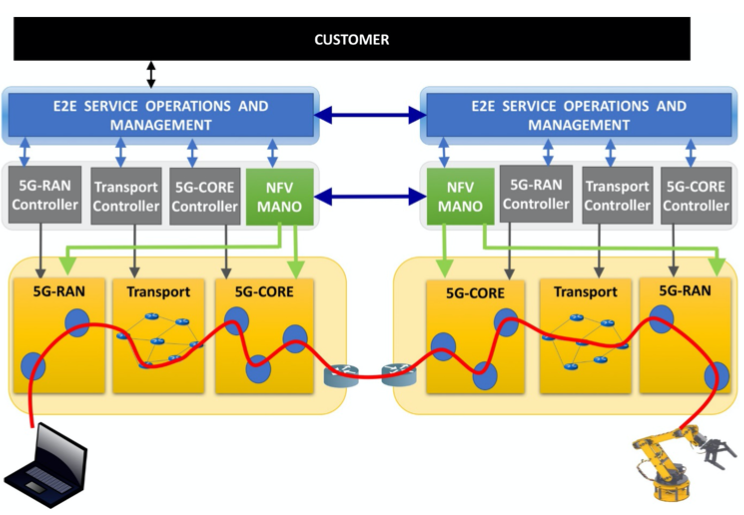
\includegraphics[width=.9\textwidth]{templates/images/chapter03/service-inter-operation.png}
        \caption{Service Inter-Operation across \acrshort{5gvinni} Sites. Source: }
        \label{service-inter-operation}
    \end{figure}  
    
    In order to enable such interoperability, the use of north-south bound and east-west bound interfaces are needed in order to guarantee the proper understanding of the service needs on each of the involved sites. While the arrows are here drawn directly to and from the \acrshort{nfv} \acrshort{mano} in the neighbour domain this will typically be realized via inter-provider \acrshort{api}s\footnote{In this regard, it is important to note also that the specifications of these inter-provider \acrshort{api}s are still at an early stage and to be considered as a key activity and work in progress by the industry forums and specification defining organizations.} (e.g. along the lines of 5GEx Project \cite{carlos_bernardos_2016_671636}).

\subsection{5G Network Slice Federation Scenarios}
This section presents two types of Network Slice Federation Scenarios. First is how an \acrshort{e2e} 5G Network slice federation is created involving Access, Transport and Core by presenting a paradigm of another project, namely the 5GinFIRE H2020 project \cite{5ginfire} and how it can be adapted for other research projects. The second presents how an \acrshort{e2e} 5G Service Level Federation can be deployed with an \acrshort{e2e} cross-domain orchestrator between facilities.
    
    \subsubsection{Network Slice Federation Across \acrshort{5gvinni} Facility Sites}
    An example scenario of \acrshort{e2e} network slice federation across three different \acrshort{5gvinni} Facility Sites is illustrated in Figure \ref{fig:e2e-deployed} which involves three facilities (e.g., Norway Site, UK Site and Spain Site) providing a single \acrshort{e2e} network slice.
    
    \begin{figure}[!ht]
        \centering
        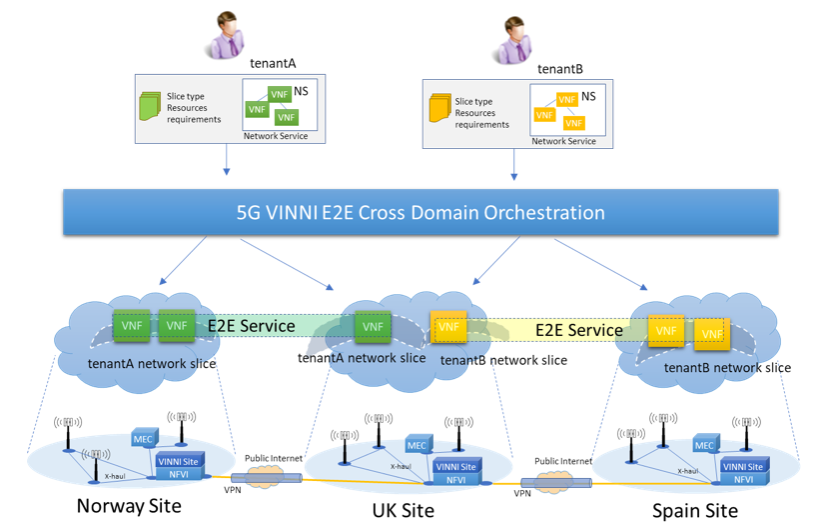
\includegraphics[width=0.9\textwidth]{templates/images/chapter03/e2e-deployed.png}
        \caption{\acrshort{e2e} Network Slice Federation across three different Facility Sites. Source: }
        \label{fig:e2e-deployed}
    \end{figure}
    
    In order to have such a scenario as per Figure \ref{fig:e2e-deployed}, the facilities would need to have established agreements in the business (e.g. what type of resources are allowed and at what cost) and connectivity level (e.g. Layer 2 or 3). With respect to the latter, related work of such deployment has been done by 5GinFIRE \cite{5ginfire} where a single \acrshort{mano} is responsible for orchestrating multiple interconnected and physically separated \acrshort{nfvi}s. In \acrshort{5gvinni}, however, each facility has its own \acrshort{mano} stack. 
    
    In 5GinFIRE, partner testbeds have mutual agreements in regards to joining and accepting NFs and also allowing access of their \acrshort{vim}'s \acrshort{api}s to a centralized \acrshort{mano}. This cross-site interconnectivity supports the exchange of control and data-plane information among sites, utilizing an overlay of a network architecture based on \acrshort{vpn}s. This approach \cite{diego_lopez_2018_732497}, given that sites are physically separated at different network locations, means that inter-site communications may traverse multiple untrusted network domains. Inter-site data-plane communications will require the creation of specific \acrshort{cim} networks at each site, with network connectivity towards the appropriate \acrshort{vpn} endpoint of the site. These networks will then be used to attach any \acrshort{vnf}s needing this type of communications, while guaranteeing all subsequent security principles. 
    
    \subsubsection{Service Level Federation across \acrshort{5gvinni} Facility Sites}
    In these scenarios, two \acrshort{5gvinni} facility sites support different types of network slices in order to create an \acrshort{e2e} service for \acrshort{5gvinni} customers. Although the federation can be seen at the Service Layer, the interconnection and interworking between the two slices would be required to support \acrshort{e2e} service operation.
  
    \begin{figure}[!ht]
        \centering
        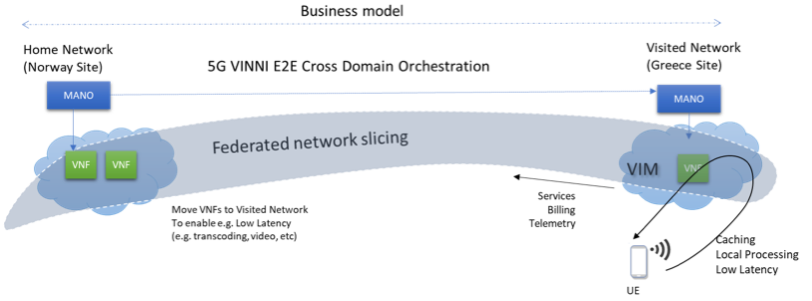
\includegraphics[width=0.9\textwidth]{templates/images/chapter03/mult-tenants.png}
        \caption{Multiple Tenants and Federated Network Slicing. Source: }
        \label{fig:multiple-tenants}
    \end{figure}     
    
    Figure \ref{fig:multiple-tenants} displays a generic view of how multiple tenants can use the \acrshort{5gvinni} \acrshort{e2e} Facility to deploy an \acrshort{e2e} service on top of a network slices types. This connectivity provides a unified service experience for the creation and roaming extension of network slices optimized for demanding scenarios. Today such scenarios are exclusibely enabled for cloud services, but with the introduction of network slice requirements, services must move to the edge. In order to ensure the performance demands, edge processing is necessary to maintain latency within limits and make sure the 5G application behaves as usual, even in roaming scenarios.

%\section{Facility-Site: Greece}
%    
%    \subsubsection{Radio Access Network (\acrshort{ran})}
%    
%    LimeNET Mini is based on Mini-PC Barebone (BRIX) platform complete with an integrated LimeSDR USB with added shielding. 
%    The hardware is fully qualified for compatibility with the LimeNET Ubuntu app store. This allows Patras University and project partners to create and deploy applications to configure the system for 5G applications with no system compatibility issues.
    
%    LimeNET Base station is a software defined radio power house. It is based on top of the line PC fitted with the newly developed LimeSDR QPCIe board. This new board is a much more sophisticated version of the LimeSDR board used in LimeNET Mini. It has two LMS7002 transceiver chips instead of one, which allows for a 4x4 MIMO configuration instead of a 2x2 MIMO configuration.
    
%    SRS primary role consists of setting up the software side of the Patras \acrshort{ran} Facility. This will include deploying a 4G software-defined network using the currently available open-source srsUE, srseNB and srsEPC products, and designing and implementing new 5G \acrshort{nr} solutions. The latter effort will span the duration of the whole project. Next, we list the several solutions SRS plans to make available and accessible in the Patras Facility by the final release of \acrshort{5gvinni}:
%    \begin{itemize}
%        \item srsUEs - software-defined \acrshort{lte} \acrshort{ue}s, capable of performing 2x2 MIMO, carrier aggregation, multicast, and handover. The srsUE will be available in the outdoor and indoor testbeds. In the outdoor testbed, it will run on LimeNET mini boards equipped with power amplifiers to sustain long distance connections. In the indoor testbed, the srsUEs will run on LimeSDR minis, with all the baseband processing performed in a laptop. 
        
%        \item srseNB - software-defined \acrshort{lte} eNB. The srseNB is currently capable of performing MIMO, multicast, and different scheduling algorithms. It will run on a LimeNET Base Station in the Patras outdoor testbed, and on a Lime SDR mini connected to a laptop in the indoor testbed.
        
%        \item srsgUE - software-defined Non-Standalone (\acrshort{nsa}) gUE, including the 5G \acrshort{nr} PHY and upper layers. It is currently in a stage of early development.
        
%        \item  srsgNB - software-defined Non-Standalone (\acrshort{nsa}) \acrshort{gnb}, including the 5G \acrshort{nr} PHY and upper layers. It is currently in a stage of early development.
%    \end{itemize}

%    Edge site is planned for Rel-1. The decision on location is not yet decided and will depend on requirements of the funded ICT-19 projects. 
%    Nevertheless, the Edge site will be included with one of the solutions presented in next figure: Either the Edge site compute nodes will be managed by OpenStack, or the Edge site will be seen as its own \acrshort{cim}, handled as a multiVIM scenario by \acrfull{osm} deployed at Patras Facility-site

%    \subsubsection{Core}
%    The 5G Mobile Core is realized by the deployment of Fraunhofer FOKUS' Open5GCore. Open5GCore is a use case-agnostic, standard compliant software-only prototype, implementing the 5G Core components and interfaces, addressing the use cases of seamless mobile broadband connectivity, multimedia and content delivery and massive \acrshort{iot}. For more details on Open5GCore please refer to the Berlin Facility-site description of this chapter. 

%    \subsubsection{Transport Infrastructure}
%    The transport network that will connect the \acrshort{ran} with the Core in the Patras Facility-site, will consist of the following connections: 
%    \begin{itemize} 
%        \item The Facility will be interconnected via a dedicated 10 Gb link with GRNET NRN in Athens that will allow high speed connectivity to public Internet but also to dedicated GEANT links or \acrshort{vpn} connections with other \acrshort{5gvinni} sites.
%        \item Point-to-Point mmWave wireless links, operating at 71-76/81-86 GHz and delivering up to 10 Gbps, will interconnect the University campus with selected sites several kilometres away, backhauling the gNBs and FWA that will serve public places in Patras sub-urban area.
%        \item Fixed Wireless Access (FWA) links at 26/28 GHz bands, providing up to 1 Gigabit Ethernet to the subscriber and up to 1.6 Gbps aggregate capacity per sector, will interconnect two buildings of public interest in Patras sub-urban area, providing access to \acrshort{5gvinni} core network services.
%    \end{itemize}
    
%    \begin{figure}[!ht]
%        \centering
%        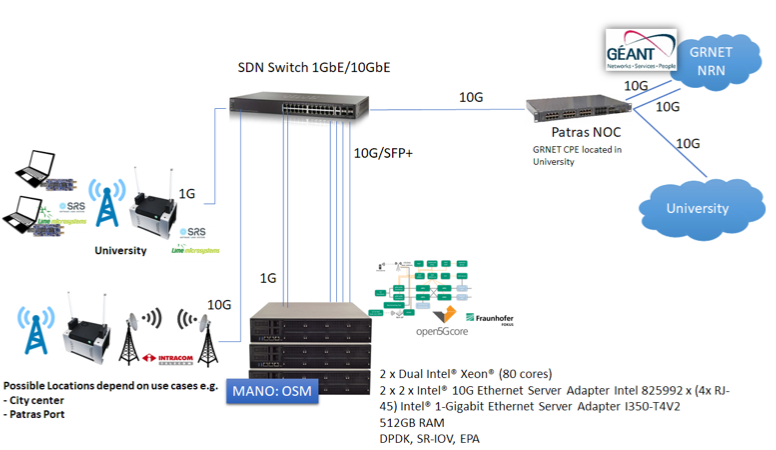
\includegraphics[width=0.9\textwidth]{templates/images/chapter03/fwa-backhaul-patras.png}
%        \caption{FWA and Backhaul Networks at Patras Facility-Site}
%        \label{fig:fwa-backhaul-patras}
%    \end{figure}
    
%    Detailed radio planning studies has been performed to identify the optimum locations, the appropriate equipment and its configuration, to provide high-speed fixed wireless access to two public services establishments, and to cover this, along with a collocated \acrshort{gnb}, with high capacity, low latency, long range backhaul. The results of these studies are listed in the LLD of the Facility.
    
%    \subsubsection{Management and Orchestration}
%    The Patras Facility uses currently OSM FOUR but will migrate to Open Source \acrshort{mano} version FIVE with OSM FIVE VNFM support 
%    \acrshort{osm} is an \acrshort{etsi}-hosted open source community delivering a production-quality \acrshort{mano} stack for \acrshort{nfv}, capable of consuming openly published information models, available to everyone, suitable for all \acrshort{vnf}s, operationally significant and \acrshort{cim}-independent. OSM is aligned to \acrshort{nfv} ISG information models while providing first-hand feedback based on its implementation experience.

%    A first approach towards this is to use the existing work from 5GinFIRE project [21] and mainly integrate for the Release 1 the 5GinFIRE portal to deploy NSs. Within 5GinFIRE some of the core functionalities that facilitate the LCM of various artefacts have been defined:
    
%    \begin{itemize}
%        \item Management of \acrshort{vnf}s, NSDs, users, infrastructures and experiments in portal
%        \item Maintain a reusable public catalog of \acrshort{vnf}s and NSDs together with versioning, licensing, etc
%        \item Description and availability of experimentation resources
%        \item Onboarding/Offboarding \acrshort{vnf}s/NSDs to multiple MANOs
%        \item Validation of \acrshort{vnf}s, NSDs
%        \item \acrshort{vnf}s Images management: These repositories contain the \acrshort{vnf} images that need to be deployed in target \acrshort{vim}s
%        \item Experimentation scheduling and deployment requests as well \acrshort{vnf} placement to multiple \acrshort{vim}s for distributed Network Services
%    \end{itemize}
    
%    \subsubsection{Security}
%    All Patras Facility infrastructure will have its own private network. The \acrshort{nfvi} infrastructure is behind a firewall with restricted access to Internet allowed only to specific services.

\newpage    
    \subsection{Use Case Verticals} 
    \label{chap:ucv}
    The \acrshort{5gvinni} facility site in Patras (Greece) will be an exemplary Open Source 5G-\acrshort{iot} facility. This means that most of the installed components will be offered as Open Source but there will be also dedicated components and services to support 5G-\acrshort{iot} scenarios. Numerous partners will deploy their technologies in the Patras/Greece facility, thus creating a unique 5G playground for \acrshort{kpi} validation and support on future verticals. 

    \subsubsection{Verticals Summary}
    Additionally, please note that these use cases could be combined and create different scenarios, by using some aspects of each distinct use cases.
    The service offerings referred in the Greece portfolio are detailed in Table \ref{tab:service-offerings} including information on their service exposure level and their ability to support the aforementioned use cases.

    \begin{table}[!ht]
       \begin{threeparttable}
    \caption{Service Offerings in the Greece Portfolio}
    \label{tab:service-offerings}
    \setlength\tabcolsep{0pt} % make LaTeX figure out intercolumn spacing
    
    \begin{tabular*}{\columnwidth}{@{\extracolsep{\fill}} lll}
    \toprule
         Service offerings & Service exposure & Supported use cases\\
    %     \multicolumn{4}{c}{Accuracy (\%)} \\ 
    %\cmidrule{3-6}
    %     & & K3 & K6 & L1 & mean\tnote{c} \\
    \midrule
          \acrshort{embb} network SaaS & Level 3-4 & UC1\tnote{1}, UC2, UC4 \\
    \addlinespace
         uRLLC network SaaS & Level 3-4 & UC1\tnote{1} \\
    \addlinespace
          mIOT network SaaS & Level 3-4 & UC3 (\acrshort{iot} slicing) \\
    \addlinespace
          Customised network slice & Level 3-4 & UC1\tnote{1}, UC3 (NB-\acrshort{iot} slicing) \\
    \bottomrule
    \end{tabular*}
    
    \smallskip
    \scriptsize
    
    \begin{tablenotes}
    \RaggedRight
    \item[1] Due to uRLLC and \acrshort{embb} characteristics, the UC1 should be executed in a customised network slice. Until this service offering becomes available in the Greece portfolio, UC1 will be executed (with some limited performance and/or functionality) in \acrshort{embb} and uRLLC network slices offered as a service to the CSC.
    \end{tablenotes}
       \end{threeparttable}
    \end{table}
    
    In Greece facility site, the following use cases are selected as the main candidates for \acrshort{5gvinni} validation purposes:
    
\newpage
    
    \subsubsection{UC1 – First Person View Remote Control Vehicle (Automotive)}
    This use case consists of a remote-controlled vehicle with an on-board camera that provides real-time video streaming, allowing for remote operating. The camera provides real time frontal view of the vehicle, so the user can steer the vehicle by means of a controller. The video streaming aspect of the use case requires a significant amount of data received through the 5G network, while the remote-control aspect requires low latency and high reliability delivery of the movement commands. To satisfy these requirements, capabilities provided by \acrshort{embb} and \acrshort{urllc} slices are critical.
\medskip
    \begin{figure}[!ht]
        \centering
        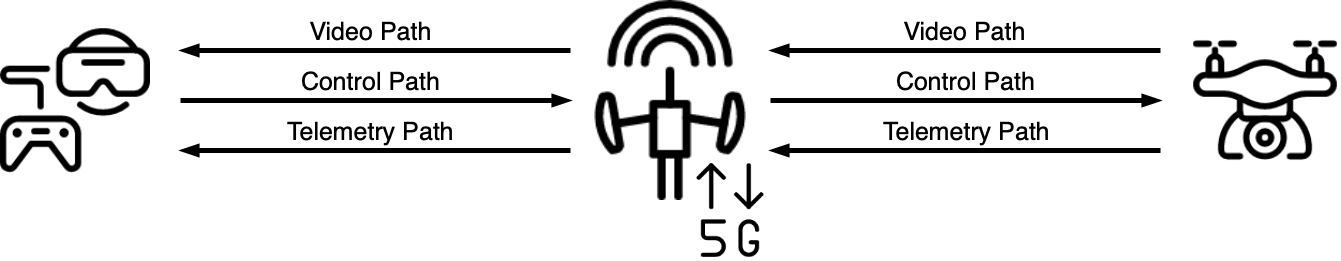
\includegraphics[width=0.9\textwidth]{templates/images/chapter03/use-case-01.png}
        \caption{Greece UC1 – First Person View Remote Control Vehicle Use Sase}
        \label{fig:uc1}
    \end{figure}     

    \subsubsection{UC2 – 360-degree Video broadcast (Media and Entertainment)}
    This use case involves video streaming with a 360-degree camera. A possible scenario is during Patras carnival festivities, where participants can be equipped with 5G-enabled devices with 360o cameras in order to transmit the local festivities to remote locations while being able to move around downtown Patras. The main requirements of this use case are high throughput and high connection density in crowded scenarios. 
\medskip
    \begin{figure}[!ht]
        \centering
        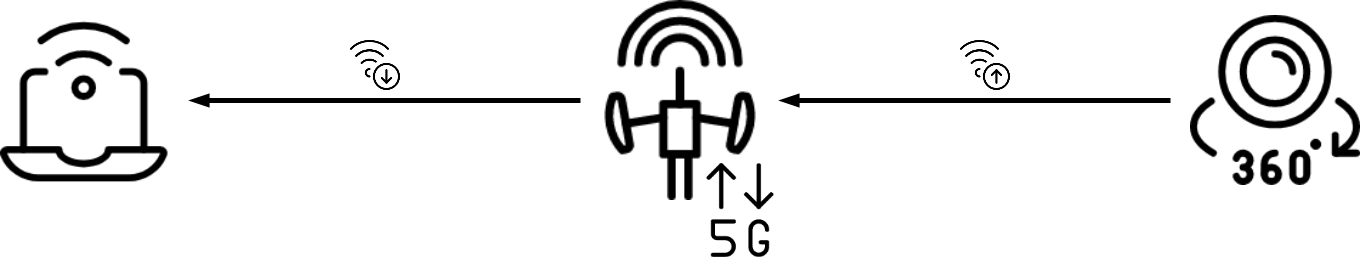
\includegraphics[width=0.9\textwidth]{templates/images/chapter03/use-case-02.png}
        \caption{Greece UC2 – 360\degree Video Broadcast Use Case}
        \label{fig:uc2}
    \end{figure}  	
\newpage
	\subsubsection{UC3 – NB-\acrshort{iot} Coverage and \acrshort{iot} Slicing study}
	The suggested use case for NB-\acrshort{iot} consists of two phases. In the first phase, a coverage study of NB-\acrshort{iot} devices will be carried out on the University of Patras (see Figure \ref{fig:uc3}). In this study, a large number of NB-\acrshort{iot} devices will be deployed and the network coverage will be examined, taking into consideration various factors including (but not limited to) distance from the antenna and penetration power. Once these factors have been analysed, then the second phase will apply the concept of \acrshort{iot} slicing, making use of distinct \acrshort{iot} applications provided by corresponding virtualized \acrshort{iot} Gateway instances deployed in separated \acrshort{nsi}s (see Figure \ref{fig:subim2}).
\medskip
    \begin{figure}[!h]
        \begin{subfigure}{\linewidth}
            \centering
            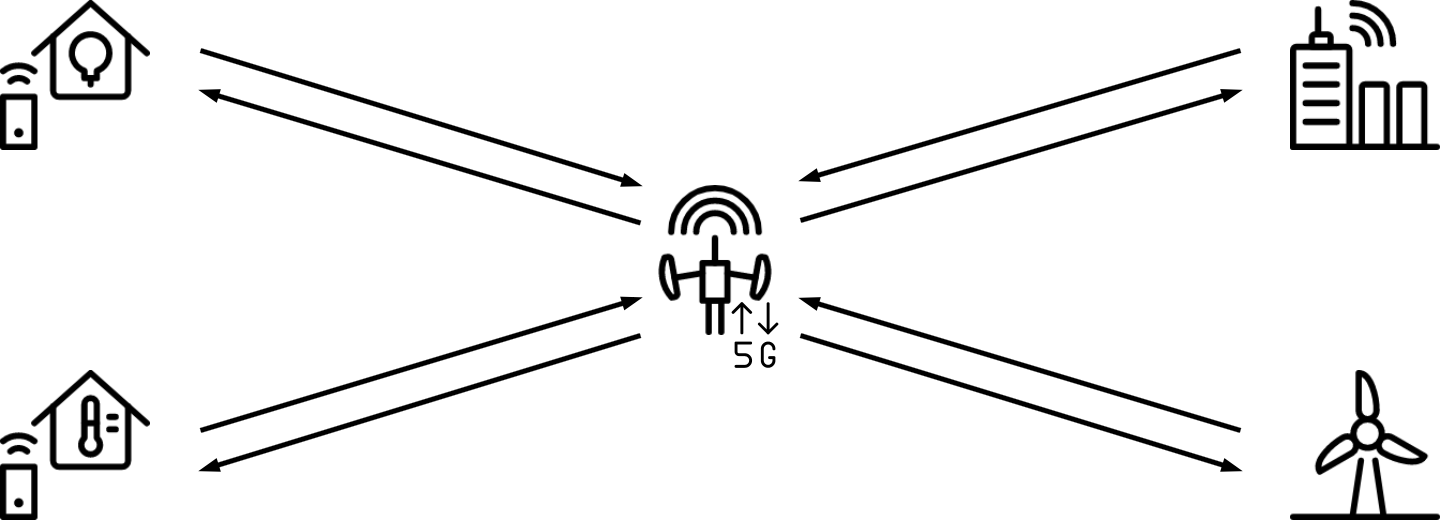
\includegraphics[width=0.9\linewidth]{templates/images/chapter03/use-case-03.png} 
            %\captionsetup{width=.9\linewidth}
            \caption{Greece UC3 – NB-\acrshort{iot} Coverage}
            \label{fig:uc3}
        \end{subfigure}
        %\hspace{10pt}
        \hfill
        \begin{subfigure}{\linewidth}
            \centering
            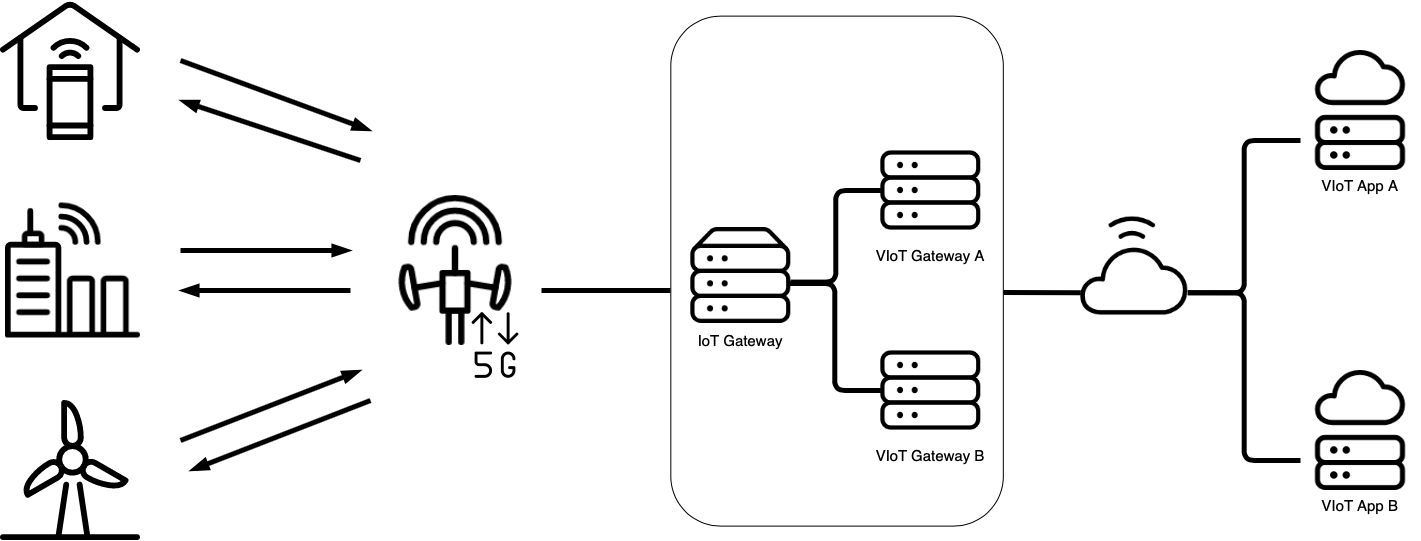
\includegraphics[width=0.9\linewidth]{templates/images/chapter03/iot-slicing-concept.png}
            \caption{Greece UC3 – Concept of \acrshort{iot} Slicing}
            \label{fig:subim2}
        \end{subfigure}
        \hfill
        \caption{Greece UC3 - Narrowband IoT Use Case}
        \label{fig:iot-slicing-concept}
    \end{figure}
\newpage	
	\subsubsection{UC4 – \acrshort{ar} Use Case (Media and Entertainment)}
	This use case describes the delivery of \acrshort{ar} annotations on top of a video stream captured by an end user of the service. The end user captures video, which is delivered to an \acrshort{ar} application backend responsible for object recognition, tracking and annotation of the video with related information. The video annotation is performed taking into account the position of the identified objects in the video and delivered as an enhanced video stream to the user. This scenarios’ main requirement is the very high throughput. To satisfy these requirements, the operator of this use case may rely on the communication capabilities provided by an \acrshort{embb} slice. This use case is expected to be supported by DFKI, as a member of the Executive Board. The exact application context will be later defined, choosing from the wide DFKI portfolio. A candidate application targets the touristic domain, providing informational annotations on top of identified monuments. The use case targets the use of a \acrshort{mec} location within the Patras facility, as a means to lower latency. 
\medskip
    \begin{figure}[!ht]
        \centering
        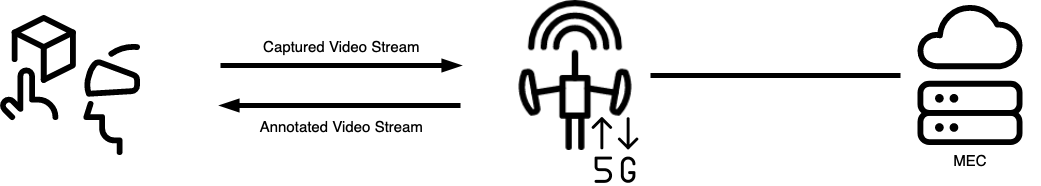
\includegraphics[width=0.9\textwidth]{templates/images/chapter03/use-case-04.png}
        \caption{Greece UC4 – \acrshort{ar} Use Case}
        \label{fig:uc4}
    \end{figure}

\chapter{Drone-based Verticals Use Case}
%% This is an example first chapter.  You should put chapter/appendix that you
%% write into a separate file, and add a line \include{yourfilename} to
%% main.tex, where `yourfilename.tex' is the name of the chapter/appendix file.
%% You can process specific files by typing their names in at the 
%% \files=
%% prompt when you run the file main.tex through LaTeX.

\section {Purpose}
This chapter will serve as an in-depth look in the general architecture and implementation steps as outlined by the 5G-VINNI principles. Below the overall setup that will comprise the first use case of the Greece main facility is documented, aiming to showcase in a practical manner the capabilities, advancements and even limitations of this paradigm shift that network slicing aims to deliver. Following this high-level yet thorough description of the main focus of this thesis, Chapter 5 will delve deeper in the configuration parameters and the actual realization of the Unmanned Aerial System (UAS) platform.
\newpage
\section {Use Case and Key Performance Indicators}
\subsubsection{Use Case Definition}
This use case briefly mentioned in Section \ref{chap:ucv} is comprised by two distinct parts that are required in order to successfully complete its task. On one end, a ground station unit will provide the user with the ability to control in real time a vehicle (in this case a quadcopter), through the cellular network. Compared to more traditional radio frequency control schemes, the user is not required to maintain line of sight of said vehicle, as the cellular-connected onboard computer is able to receive commands through the network. This leads us to the other part of the system which is of course the vehicle itself, able to transmit live video feeds back to the ground station in order to provide the user with appropriate feedback of its course, to which he can react accordingly. Legacy systems utilize alternative radio frequency bands to transmit said video feeds which are prone to interference, low quality and medium to high latency. These get replaced with modern technologies that alleviate all of the issues previously mentioned. By leveraging V2X connectivity, the user stands to benefit from the emerging 5G NR network, as increased coverage, low latency and quality of service are some of its main attributes. Such scenarios can be encountered in many cases with the most notable ones being search and rescue operations, remote takeover of autonomous vehicles or even human supervision of areas of interest. 

Design-wise, the use case requires the implementation of the user and vehicle-side aspects while simultaneously satisfying network and open-source platform requirements. As and added bonus, various accessories that can augment the overall experience such as first person view (FPV) goggles and 360o cameras shall be supported in future iterations. 

\newpage

\subsubsection {Key Performance Indicators (KPI) Definition}
As previously mentioned, this use case aims to primarily showcase the benefits provided by network slicing technologies, as its implementation on current cellular network technologies would be impossible or to the least, impractical. For said reason, we need to establish some of the main key performance indicators that will need to be achieved in order to achieve full functionality of the platform. These are briefly listed below:
\begin{itemize}
    \item Throughput: The minimum data rate required for the end-user to receive video feedback of adequate quality\footnote{For the use case High Definition (HD) quality with 24 frames per second (FPS) should be supported. This equals to a minimum throughput requirement of approximately 5 Mbps.} and latency for the use case. 
    \item Latency: This equates to the maximum end-to-end delay \footnote{No more than the latency experienced by legacy remote controlled systems.} from when the user issues a command to when the vehicle is able to receive said information and respond accordingly.
    \item Reliability: The resilience of said communications system to all kind of errors introduced by interference and channel imperfections.
    \item Service Instantiation Time: The delay measured by the time that is required by the platform to initiate, configure and deploy said required service on command.
    \item Coverage: The area\footnote{No more than 90m$^2$ will suffice for demonstration purposes. This implies that a basic off the shelf device an be utilized as a base station without requiring additional amplification and a range of about 15m.} for which the vehicle will be able to fully operate within, while still adhering to the full specifications mentioned above.  
    Area for which the vehicle will be able to move and stream video. The control path can potentially be done remotely as well.
\end{itemize}
\newpage
\section {Communication paths}
The main communication paths will be:
\begin{itemize}
    \item Video path: 
    Providing adequate bandwidth and latency for live video streaming from the vehicle to the user.
    \item Telememetry path: 
    Providing information regarding the vehicle status.
    \item Telecommand path: 
    Enabling remote vehicle operation from the user.
\end{itemize}

    \begin{figure}[!ht]
        \centering
        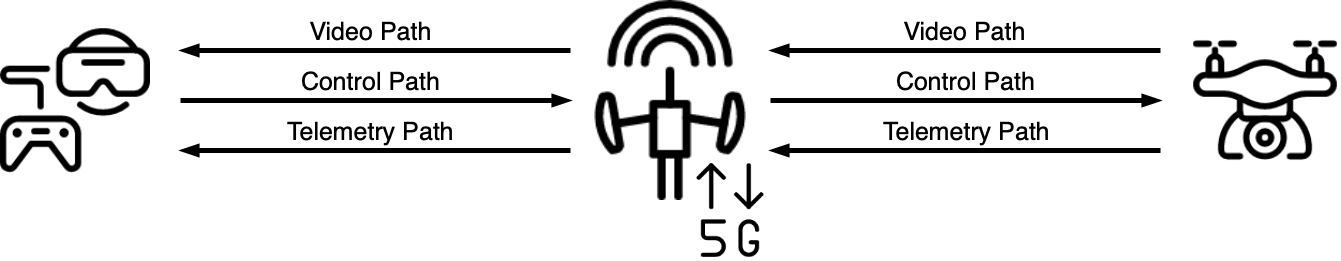
\includegraphics[width=1\textwidth]{templates/images/chapter04/use-case-scenario.png}
        \caption{Use Case Scenario}
        \label{fig:uc-scenario}
    \end{figure} 

In our use case we need to satisfy eMBB (to allow seamless video streaming) and uRLLC to enable an acceptable remote control of the vehicle.

\subsubsection {Video Path} 
The deployed 5G network must be able to successfully handle various video streams from the devices, satisfying bandwidth requirements. The user must be able to download (Rx) while the vehicle side must be able to upload (Tx) at similar rates to carry out the use case demo successfully. It goes without saying that the xNodeB should support at minimum these values in both directions. The values in Table \ref{tab:video-bw} are calculated by using 24 FPS which is considered acceptable for video streaming. Consequently, should the use case require true FPV or VR/AR, more FPS and/or higher quality, more bandwidth would be required.

\begin{table}[!ht]
   \begin{threeparttable}
\caption{Bandwidth in Relation to Video Quality}
\label{tab:video-bw}
\setlength\tabcolsep{0pt} % make LaTeX figure out intercolumn spacing

\begin{tabular*}{\columnwidth}{@{\extracolsep{\fill}} cl}
\toprule
     Bandwidth (Mbps)\tnote{1} & Usage scenario \\
\midrule
      0.5 &Minimum bandwidth required for live streaming \\
\addlinespace
     1.5 &Minimum bandwidth required for a broadband connection \\
\addlinespace
      3.0 &Standard Definition (SD) bandwidth \\
\addlinespace
      5.0 &High Definition (HD) bandwidth \\
\addlinespace
      25 &Ultra HD (4K UHD) bandwidth \\
\bottomrule
\end{tabular*}

\smallskip
\scriptsize

\begin{tablenotes}
\RaggedRight
\item[1] Due to uRLLC and eMBB characteristics, the UC1 should be executed in a customised network slice. Until this service offering becomes available in the Greece portfolio, UC1 will be executed (with some limited performance and/or functionality) in eMBB and uRLLC network slices offered as a service to the CSC.
\end{tablenotes}
   \end{threeparttable}
\end{table}
    
\newpage    
    
\subsubsection {Telecommand Path}
Depending on the type of vehicle used, the 5G solution should exhibit the same or less latency of transmission and reception of commands than traditional radio control solutions. This would allow for a paradigm shift in either reduced latency, theoretically unlimited range or both, over legacy systems.

\subsubsection {Telemetry Path}
The telemetry path aims to showcase an optional implementation of a mIoT slice for a less-demanding path in terms of network resources. Telemetry data such as drone location, altitude and orientation would prove extremely vital for flight path logging, as well as any potential use case specific sensors that could be mounted to the drone platform at each time.

%\newpage

\section {System Architecture Overview}
A more thorough description of the use case is provided on the next sections. Please note that final implementation concepts or hardware can vary, but the overall system architecture will remain the same.
\newpage
\subsection {User Side}
For the User Side, a configuration as shown in Figure \ref{fig:detailed-approach-user} is proposed:

    \begin{figure}[!ht]
        \centering
        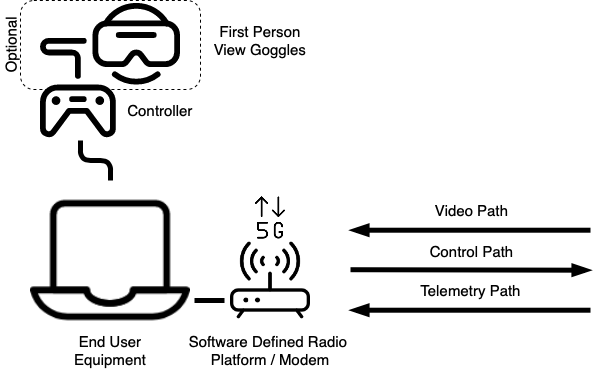
\includegraphics[width=0.9\textwidth]{templates/images/chapter04/detailed-approach-user.png}
        \caption{Detailed Approach for User Side of Use Case}
        \label{fig:detailed-approach-user}
    \end{figure} 

In our use case scenario, the goggles are replaced with a laptop for the sake of simplicity. This is in part for removing an extra layer of complexity from the development cycle and mainly for the reason that no 5G-compatible standalone headsets exist commercially. Most of the currently available products either use radio frequencies on the 2.4 or 5.8 GHz bands, suffering of course greatly from reduced range and reception quality. In future iterations, the First Person View goggles could be connected to a video out port on the end user equipment (in this case a laptop) to alleviate this problem. 
Due to the nature of analog control of vehicles, the laptop keyboard should be avoided as a means of steering at all costs, as it would prove too "rough" of an input device (either full throttle or none). For this reason, a wireless adapter will be used to relay a traditional two-stick radio controller's commands to the ground station software running on the laptop. Commercial joysticks aimed for video game use have demonstrated allot of jitter on their input so they are also disqualified for the sake of safety of both the drone and the pilot.
%In terms of processing power, the laptop could possibly be replaced with a thin client, for the sole reason that only decoding of the incoming video stream and transmission of low-bandwidth control commands would be required. %Greater attention should be put onto its networking capabilities and quality of screen for outdoor scenarios, but this is outside of the scope of this work.

\subsection {Vehicle Side}
Regarding the vehicle side, the following setup is proposed:

    \begin{figure}[!ht]
        \centering
        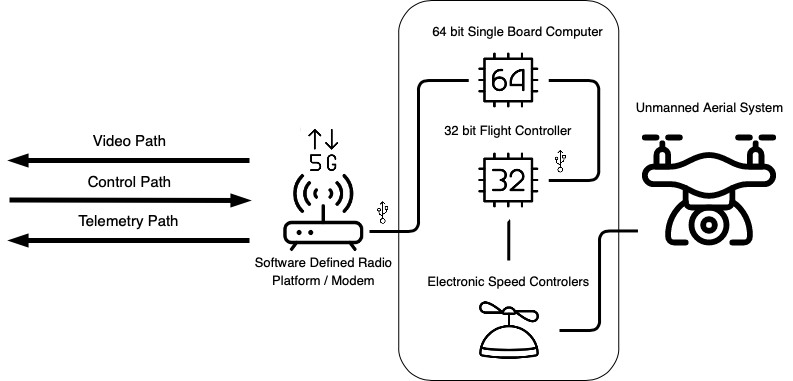
\includegraphics[width=1\textwidth]{templates/images/chapter04/detailed-approach-vehicle.png}
        \caption{Detailed Approach for Vehicle Side of Use Case}
        \label{fig:detailed-approach-vehicle}
    \end{figure} 

One of the most important parts of the use case is the vehicle side implementation. This is because all workload-intensive tasks such as video encoding and streaming while maintaining timely reaction to received commands are vital to its operation. For this reason, commercial off-the-shelf solutions that are geared towards recreational usage prove to be severely incapable of conforming to our platform needs. After extensive market research, only two solutions satisfied all the demands that our use case would require, those being either a custom-made solution from readily available parts or a drone research kit offered by Intel. Both of those proved to have their own distinct advantages, but the Ready to Fly (RtF) solution was preferred over the tedious task of tinkering with PID controllers and troubleshooting hardware bugs.
In short, the Intel Aero platform provides a powerful, yet light enough Single Board Computer (SBC) for video encoding and streaming, as well as a combined takeoff weight of 1.9kgs. This would allow for more than enough headroom for future expansions, as additional cameras or sensors and easily be mounted and still maintain nominal 20 minutes flight time. Finally, the kit comes bundled with Intel's own flight controller, that connects over a serial port to the companion computer.% and offers the ability to send and receive control commands over any network or interface, proving especially useful for our implementation.

\newpage

\section {Intermediate Implementation Steps}
\subsubsection {Step 1}
%The setup seen on Figure \ref{fig:impl-step1} could be used at the first phase of implementation
By only using laptops, the first step ensures the integrity of communication between the UE through the experimental cellular network.

    \begin{figure}[!ht]
        \centering
        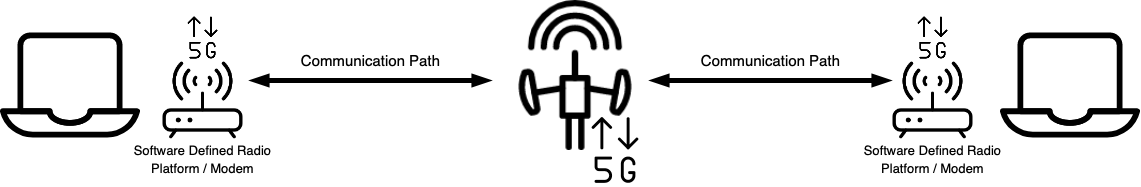
\includegraphics[width=0.9\textwidth]{templates/images/chapter04/impl-step-01.png}
        \caption{Implementation Step 1 - Verify Communication}
        \label{fig:impl-step1}
    \end{figure} 

\subsubsection {Step 2}
Using the same setup as before, replacing data with a complete video streaming pipeline between the UE and ground station in order to verify its quality.

    \begin{figure}[!ht]
        \centering
        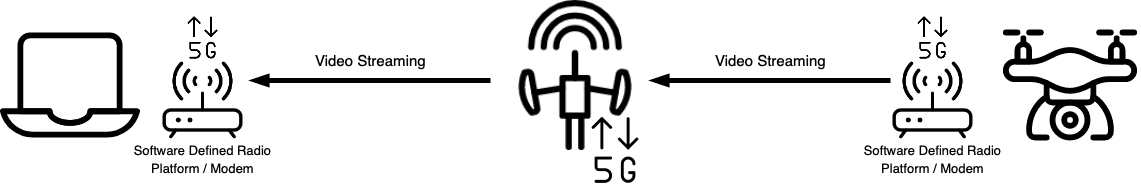
\includegraphics[width=0.9\textwidth]{templates/images/chapter04/impl-step-02.png}
        \caption{Implementation Step 2 - Verify Streaming}
        \label{fig:impl-step2}
    \end{figure}
    
\subsubsection {Step 3}
Finally, replacing the laptop with a \acrfull{sbc}, will allow to verification of the minimum system requirements. Simultaneously, the flight controller module can be also tested to verify cohesion of the control path.

    \begin{figure}[!ht]
        \centering
        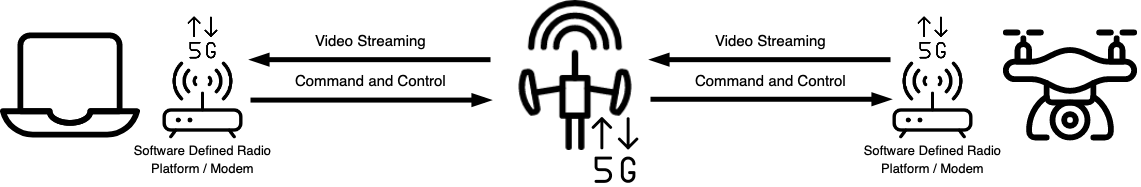
\includegraphics[width=0.9\textwidth]{templates/images/chapter04/impl-step-03.png}
        \caption{Implementation Step 3 - \acrshort{sbc} Requirements and Remote Control}
        \label{fig:imple-step3}
    \end{figure} 
\newpage

\section {Suggested Hardware}
The combination of digital processing and analog RF has always made up communication systems. In today's modern systems signal processing has progressed to such an extent that a majority of baseband functionality is being implemented in software. The flexibility of the RF hardware to be re purposed and reconfigured has led to one radio font-end handling most RF systems. Normally the RF front-end is software controlled rather than software defined. This modern combination of flexible RF front-ends and signal processing in software has lead to the birth of software-defined radio. In general, a digital communications system consists of an interdependent sequence of operation responsible for taking some type of information and transmits it over-the-air to a receiver for processing and decoding into a reconstructed version of the original information signal.

There has been a growing amount of interest with respect to combining SDR technology with software-defined networks (SDNs), where the latter focuses on adapting the higher communication layers to the prevailing operational environment. This enables things like modification of the routing to be tied to heuristiccs provided by the physical layers. 

Next-generation communications systems introduce new challenges that require solutions beyond what can be achieved through individual device optimization. Integrating more software control and cognitive abilities to the radio demands a more frequency- and bandwidth-flexible RF design. To achieve this goal static filters need to be removed and replaced with tunable filters. Similarly, the concept of a common platform would allow for shorter development times, reduced manufacturing costs, and provide greater interoperability between systems. The common platform demands that the RF system be capable of providing full performance for applications that traditionally had very different architectures. Finally, future platforms are pushing size and power demands to a new extreme.

\subsection {Suggested Hardware for xNodeB}
For this reason design considerations to take into account when devising digital communication systems based on an SDR platform include the integration of the physical and network layers via a real-time protocol implementation of an embedded processor. Most communication systems are divided into logically separated layers in order to more readily facilitate the design of the communication system. However, it is imperative that each layer is properly designed due to the strong interdependence between all the layers. Ensuring that a sufficiently wide bandwidth radio front-end exists with agility over multiple subchannels and a scalable number of antennas for spatial processing. Many networks employing digital communication systems possess a centralized architecture for controlling the operations of the overall network. Knowing the radio network architecture is important since it will dictate what sort of operations are essential for one digital transceiver to communicate with another. The ability to perform controlled experiments in different environments is important for the sake of demonstrating the reliability of a particular SDR implementation, providing a sanity check capability. Reconfigurability and fast prototyping through a software design flow for algorithm and protocol description. 

From the perspective of a radio system and its implementation, much of the system design will focus on the physical layer, but it can't be forgotten how the link layer may affect the physical. Nevertheless, given that the baseband processing is all conducted in software, it is possible for the communications system to implement the higher layers of the stack in software as well. Many communication standards have adopted this scheme, where the entire communication system across all the layers are implemented in software, although depending on data rate requirements, this can require significant computational capabilities on the part of the system to achieve real-time operation. All software implementation enable functional updates without hardware replacements.The trade-offs of which function or layer is done in fixed hardware versus flexible software is an engineering decision based on volume, cost , power, complexity and many other factors. 
%software defined radio for engineers, p.8

\begin{sidewaystable*}
    \begin{threeparttable}
    \scriptsize
        \caption{Software Defined Radio Platforms for xNodeB}
        \label{tab:sdr-xnodeb}
    \begin{tabularx}{\textwidth}{@{}l*{10}{C}c@{}}
    \addlinespace
    \toprule
     & Range (MHz) & Bandwidth (MHz) & Rx/Tx & Duplex & Tx Power (dBm) & Sampling (MSps) & Interface & Chipset (FPGA) &  Gates (K) & Size (mm)  & Price (USD)\\ 
     \addlinespace
        \midrule
        \addlinespace 
        USRP N210 & - & - & - & - & 15 & 100 & 1x 1Gb & DSP3400 & 6 & Half RU & 2,048\\  
        USRP N300 & 10 - 4400 & 100 & 2/2 & Full & 18 & 153.6 & 2x SFP+ & Zynq7035 & 275 & Half RU & 6,850\\ 
        USRP N310 & 10 - 6000 & 100 & 4/4 & Full & 18 & 153.6 & 2x SFP+ & Zynq7100 & 444 & Half RU & 10,537\\ 
        USRP N320 & 3 - 6000 & 200 & 2/2 & Half & 18 & 153.6 & 1xQSFP+ & Zynq7100 & 444 & Half RU & 12,000\\
        USRP N321 & 3 - 6000 & 200 & 2/2 & Half & 18 & 153.6 & 1xQSFP+ & Zynq7100 & 444 & Half RU & 13,500\\
        \addlinespace
        USRP X300 & - & - & - & - & 10 & 200 & 2x10Gb & XC7K325T & 326 & 277x218x39 & 4,640\\
        USRP X310 & - & - & - & - & 10 & 200 & 2x10Gb & XC7K410T & 407 & 277x218x39 & 5,714\\  
        \addlinespace
        USRP E310 & 70 - 6000 & 56 & 2/2 & Full & 10 & 61.44 & 1x1Gb & Zynq7020 & 85 & 133x68.2x26 & 3,221\\
        USRP E313 & 70 - 6000 & 56 & 2/2 & Full & 10 & 61.44 & 1x1Gb & Zynq7020 & 85 & 186x280x106 & 4,334\\
        \addlinespace
        LimeSDR & 0.1 - 3800 & 61.44 & 2/2 & Full & 10 & 61.44 & USB 3.0 & Cyclone 4 & 40 & 100x60 & 315\\
        LimeSDR QPCIe & 0.1 - 3800 & 61.44 & 4/4 & Full & 10 & 61.44 & PCIe x4 & Cyclone 4 & 80 & 136,85x68,9 & 799\\
        LimeNET Micro & 0.1 - 3800 & 61.44 & 2/2 & Full & 10 & 61.44 & USB 2.0 & Cyclone 4 & 40 & 125x65 & 345\\
        LimeNET Mini & 0.1 - 3800 & 61.44 & 2/2 & Full & 10 & 61.44 & 1x 1Gb & Cyclone 4 & 40 & 110x105 & 2,799\\
        LimeNET Base Station & 0.1 - 3800 & 61.44 & 4/4 & Full & 10 & 61.44 & 2x 1Gb & Cyclone 4 & 40 & 265x270x260 & 21,250\\
        LimeNET CrowdCell & 0.1 - 3800 & 61.44 & 2/2 & Full & 10 & 61.44 & 1x 1Gb & Cyclone 4 & 40 & N/A & N/A\\
        \addlinespace
        \midrule
        \addlinespace
        SBX 782761 & 400 - 4400 & 40 & 1/1 & Full & - & - & - & - & - & - & 573\\  
        SBX 783351 & 400 - 4400 & 120 & 1/1 & Full & - & - & - & - & - & - & 688\\  
        \addlinespace 
        CBX 782760 & 1200-6000 & 40 & 1/1 & Full & - & - & - & - & - & - & 573\\ 
        CBX 783353 & 1200-6000 & 120 & 1/1 & Full & - & - & - & - & - & - & 688\\
        \addlinespace 
        UBX 783774-01 & 10 - 6000 & 40 & 1/1 & Full & - & - & - & - & - & - & 1,056\\  
        UBX 783775-01 & 10 - 6000 & 160 & 1/1 & Full & - & - & - & - & - & - & 1,291\\
        \addlinespace 
        TwinRX & 10 - 6000 & 80 & 2/0 & Half & - & - & - & - & - & - & 2,890\\
        \addlinespace
        \midrule
    \end{tabularx}
    \begin{tablenotes}
        \RaggedRight
        \item[1] https://www.intel.com/content/dam/www/programmable/us/en/pdfs/literature/pt/cyclone-iv-product-table.pdf.
        \item[2] Amplification.
        \item[3] Max stated, may vary in MIMO configuration .
        \item[4] additional daughterboards required.
        \item[5] small cell form-factor.
    \end{tablenotes}

    \end{threeparttable}
\end{sidewaystable*}

The USRP N310 is a networked software defined radio (SDR) that provides reliability and fault-tolerance for deployment in large-scale and distributed wireless systems. It simplifies control and management of a network of radios by introducing the unique capability to remotely perform tasks such as updating software, rebooting, factory resetting, self-testing, host PC/ARM debugging and monitoring system health. The USRP N310 is one of the highest channel density devices in the SDR market, offering four RX and four TX channels in a half-wide RU form factor. The RF front end uses two AD9371 transceivers, the latest RFIC technology from Analog Devices. Each channel provides up to 100 MHz of instantaneous bandwidth and covers an extended frequency range from 10 MHz to 6 GHz. The open-source USRP Hardware Driver (UHD) API and RF Network-on-Chip (RFNoC) FPGA development framework reduces software development effort and integrates with a variety of industry-standard tools. The baseband processor uses the Xilinx Zynq-7100 SoC to deliver a large user-programmable FPGA for real-time and low-latency processing and a dual-core ARM CPU for stand-alone operation. Users can deploy applications directly on to the preinstalled embedded Linux operating system or stream samples to a host computer using high-speed interfaces such as 10 Gigabit Ethernet over the two SFP+ ports.

Additionally, the USRP N310 has a flexible synchronization architecture with support for traditional SDR synchronization methods such as clock reference, PPS time reference, and GPSDO, which enable implementation of high channel count MIMO systems. In addition, the USRP N310 uniquely features Ethernet-based synchronization using the open-source White Rabbit timing protocol which enables precise baseband synchronization over large distances in GPS-denied environments. All Ettus Research USRP SDRs and NI USRP SDRs are supported by the USRP Hardware Driver, which is published by NI under open-source licenses. This driver facilitates application development on USRP hardware and offers cross-platform support for multiple industry-standard development environments and frameworks. As dual-licensed software, the USRP Hardware Driver is available under the open-source GNU General Public License version 3 (GPLv3).%ni.com/sdr blabla & N310 product page

\begin{figure}
    \centering
    \subfloat[Isometric view of the N310]{
      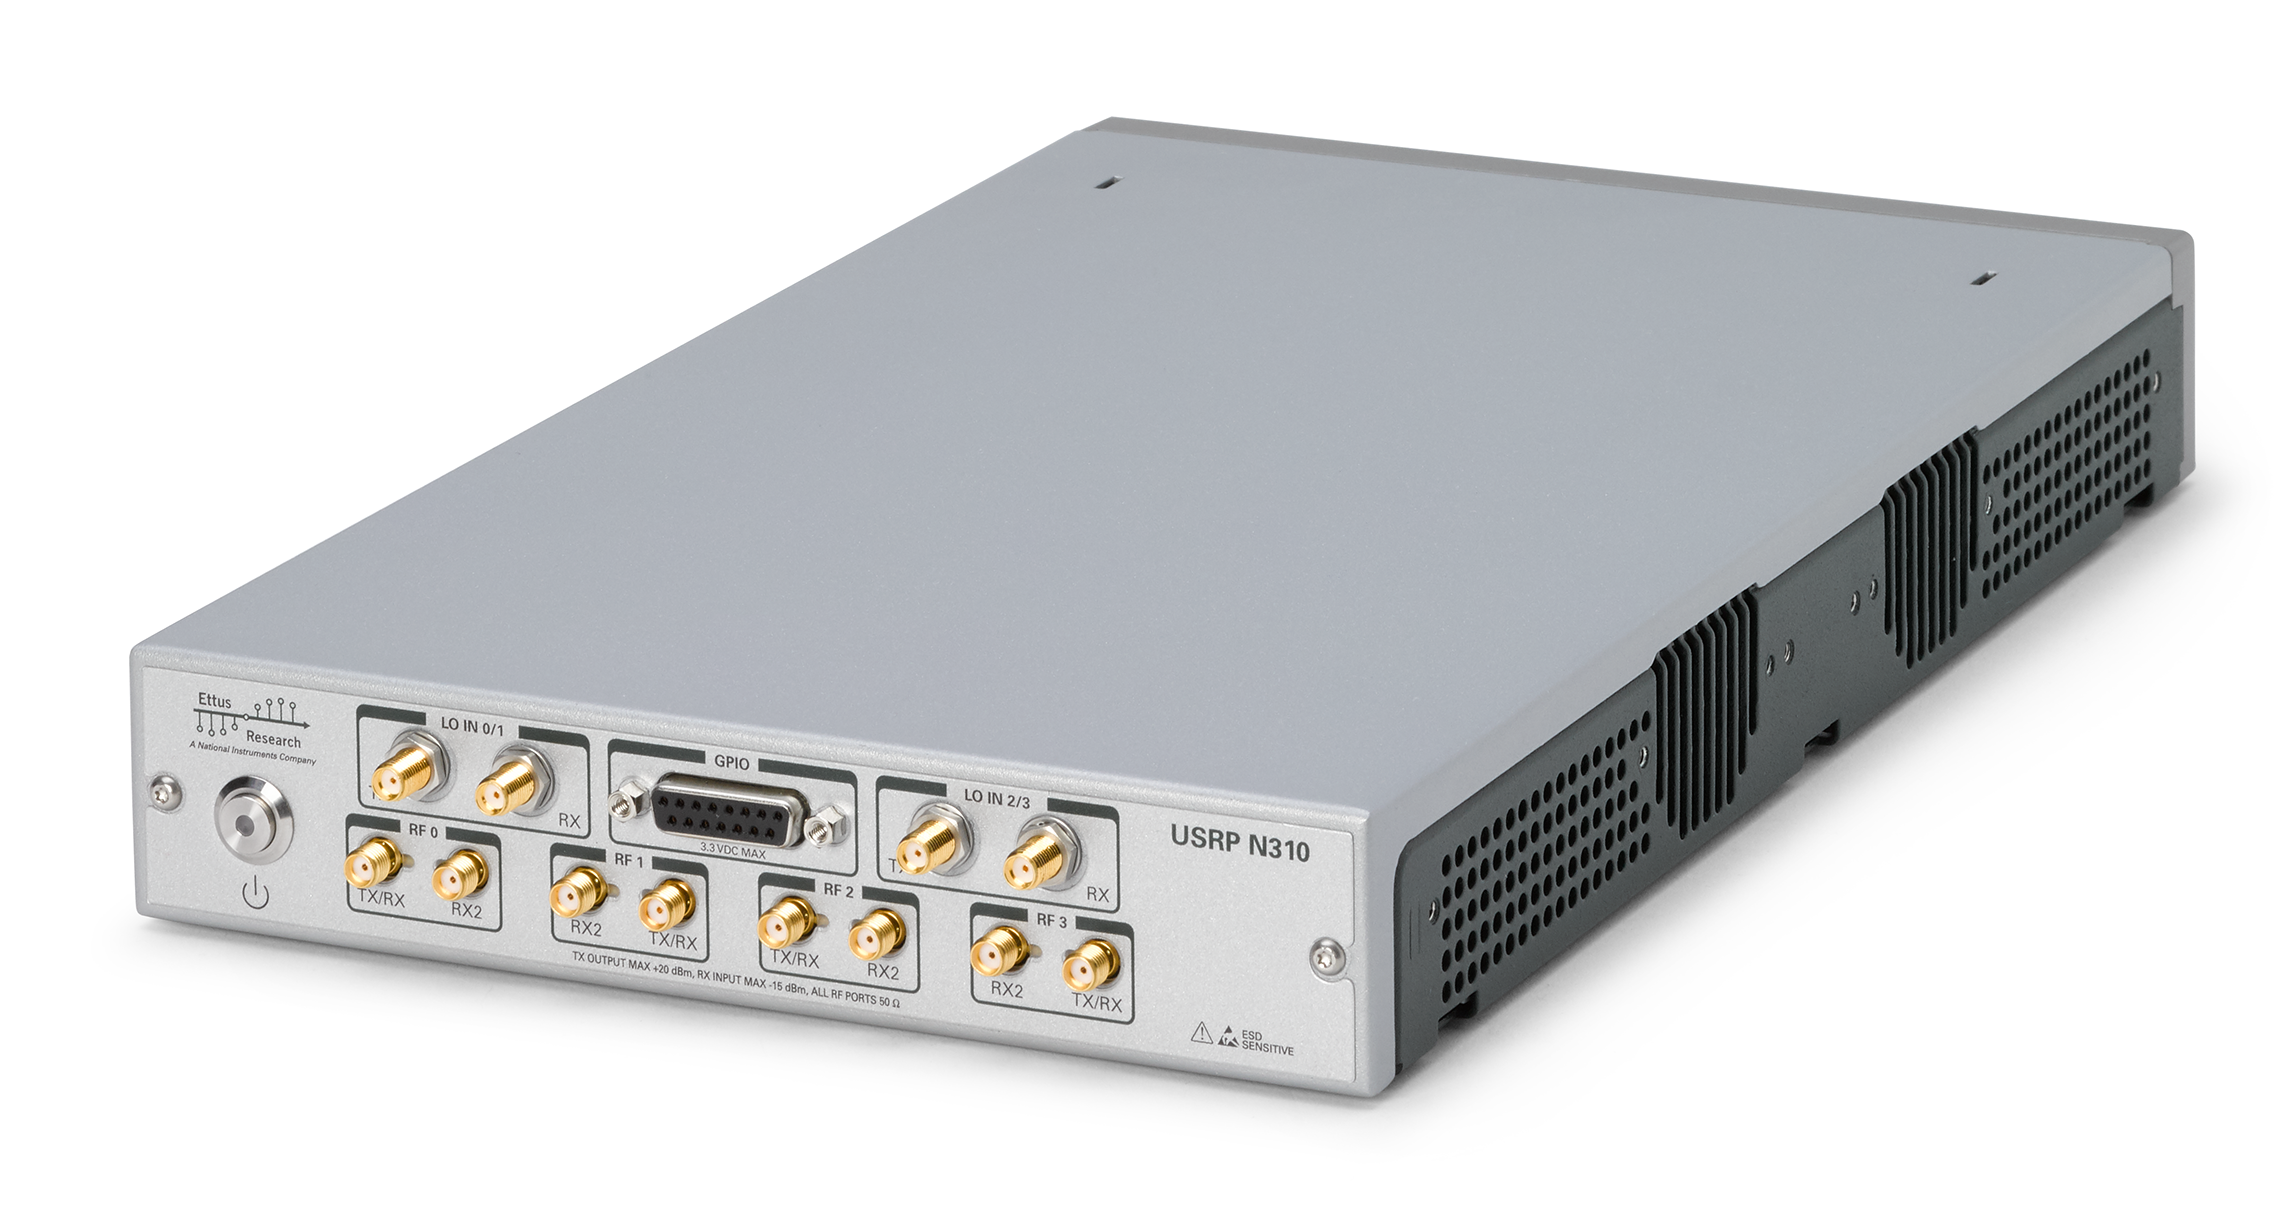
\includegraphics[width=0.9\textwidth]{templates/images/chapter05/N310_Iso-e1550871338956.png}%
      }\par
    \subfloat[Front side connectors]{%
      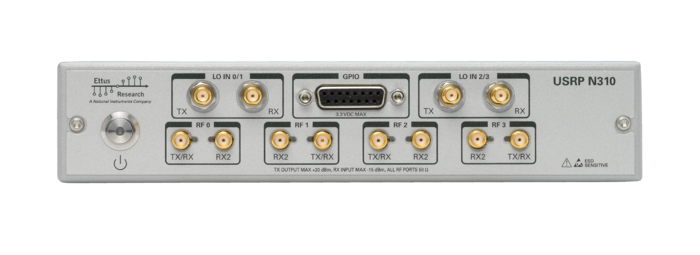
\includegraphics[width=0.9\textwidth]{templates/images/chapter05/700px-n310_front.png}%
      }\par        
    \subfloat[Back side connectors]{%
      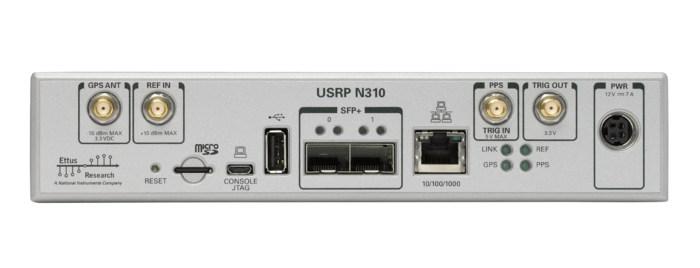
\includegraphics[width=0.9\textwidth]{templates/images/chapter05/700px-n310_back.png}%
      }
    \caption{View of the N310 SDR platform. Source: \cite{ettus-n310}}
    \label{TS}
\end{figure}
    
\newpage
%\subsection {Suggested Hardware for User Side}
%Handheld radios are becoming more capable and complex, but simultaneously requiring improved battery efficiency. Small UAVs lack the power generation of large aircraft and every milliwatt that the RF system consumes directly translates to payload battery weight, and thus, reduced flight time. To overcome these challenges and create the next generation of aerospace and defense solutions, a new radio architectures are being developed.
%Since its inception, the superheterodyne architecture has been the backbone of radio design. Whether it is a handheld radio, unmanned aerial vehicle (UAV) data link, or a signal intelligence receiver, the single or dual mixing stage superheterodyne architecture is the common choice with significant gains in performance across the entire signal chain. Microwave and RF devices have improved their performance while decreasing power consumption. ADCs and DACs have increased the sample rate, linearity, and effective number of bits (ENOB). Processing capability in FPGAs and DSPs have abide by Moore’s law, allowing for more efficient algorithms, digital correction, and further integration. Package technology has shrunk device pin density while simultaneously improving thermal handling.
%However, these device-specific improvements are beginning to reach the point of diminishing returns. While the RF components have followed a reduced size, weight, and power (SWaP) trend, high-performance filters remain physically large and are often custom designs, adding to overall system cost. Additionally, the IF filters set the analog channel bandwidth of the platform, making it difficult to create a common platform design that can be reused across a wide range of systems. For package technology, most manufacturing lines will not go below a sub-mm ball pitch, placing a limit on how physically small a complex device with many I/O requirements can become.
%software defined radio for engineers, p.10

%\begin{sidewaystable*}
%    \begin{threeparttable}
%    \scriptsize
%        \caption{Software Defined Radio Platforms for }
%        \label{tab:sdr-ue}
%    \begin{tabularx}{\textwidth}{@{}l*{10}{C}c@{}}
%    \addlinespace
%    \toprule
%     & Frequency Range(MHz) & Channel BW(MHz) & Rx/Tx & Duplex (Full/Half) & N. Figure  (dB) & Sample  (MSps) & Interface & Chipset (FPGA) &  Gates (k) & Size (mm)  & Price  \\ 
%     \addlinespace
%        \midrule
%        \addlinespace 
%        USRP B200 & 70-6000 & 56 & 1/1 & Full & 8 & 61,44 & USB 3.0 & XC6SLX75 & 75 & 97x155x15 & 785\\
%        USRP B210 & 70-6000 & 56 & 2/2 & Full & 8 & 61,44 & USB 3.0 & XC6SLX150 & 147 & 97x155x15 & 1,282\\
%        \addlinespace 
%        USRP B200mini & 70-6000 & 56 & 1/1 & Full & 8 & 61,44 & USB 3.0 & XC6SLX75 & 75 & 83.3x50.8x8.4 & 807\\
%        USRP B200mini-i & 70-6000 & 56 & 1/1 & Full & 8 & 61,44 & USB 3.0 & XC6SLX75 & 75 & 83.3x50.8x8.4 & 932\\
%        USRP B205mini-i & 70-6000 & 56 & 1/1 & Full & 8 & 61,44 & USB 3.0 & XC6SLX150 & 147 & 83.3x50.8x8.4 & 959\\
%        \addlinespace 
%        LimeSDR & 10 - 3800 & 61.44 & 2/2 & Full & 3.5 & 61.44 & USB 3.0 & Cyclone 4 & 40 & Vendor & 315\\
%        LimeSDR Mini & 10 - 3500 & 30.72 & 1/1 & Full & 3.5 & 30.72 & USB 3.0 & MAX 10 & 16 & 69x31.4 & 175\\
%        \addlinespace 
%        XTRX CS & 30 - 3700 & 120 & 2/2 & Full & 3.5 & 3.5 & PCIe x2 &  XC7A35T & 33 & Mini PCIe & 260\\
%        XTRX Pro & 30 - 3700 & 120 & 2/2 & Full & 3.5 & 3.5 & PCIe x2 &  XC7A50T & 52 & Mini PCIe & 599\\
%        \addlinespace
%        \midrule
%    \end{tabularx}
%    \begin{tablenotes}
%        \RaggedRight
%        \item[1] For users in vehicles, the UE can be connected to the network directly, or via an on-board moving base station.
%        \item[2] A certain traffic mix is assumed; only some users use services that require the highest data rates [2].
%        \item[3] For interactive audio and video services, for example, virtual meetings, the required two-way end-to-end latency (UL and DL) is 24 ms while the corresponding experienced data rate needs to be up to 8K 3D video [300 Mbps] in uplink and downlink.
%        \item[4] These values are derived based on overall user density. Detailed information can be found in [10].
%    \end{tablenotes}

%    \end{threeparttable}
%    \end{sidewaystable*}
\newpage
%\subsection {Suggested Hardware for Vehicle Side}
%<*Intel Aero>

%MAVLink or Micro Air Vehicle Link is a protocol for communicating with small unmanned vehicle. It is designed as a header-only message marshaling library. MAVLink was first released early 2009 by Lorenz Meier under LGPL license. It is used mostly for communication between a Ground Control Station (GCS) and Unmanned vehicles, and in the inter-communication of the subsystem of the vehi- cle. It can be used to transmit the orientation of the vehicle, its GPS location and speed.
%This will be the primary means of communication between the onboard computer and the dedicated autopilot module. [https://www.intel.com/content/dam/support/us/en/documents/boardsandkits/aero/ apu-161110-pixhawk-flight-guide.pdf] This way, the user will be able to control the vehicle remotely with a simple TCP or UDP connection, as-well as get instant telemetry feedback, by configuring ap- propriately the autopilot’s ports. [http://ardupilot.org/copter/docs/common-telemetry-port-setup-for- apm-px4-and-pixhawk.html]

\newpage

\section {Bill of Materials (BOM)}

\begin{table}[H]
   \begin{threeparttable}
\caption[Suggested Bill of Materials] {(BOM)}
\label{tab:equipment-list}
\setlength\tabcolsep{0pt} % make LaTeX figure out intercolumn spacing

\begin{tabular*}{\columnwidth}{@{\extracolsep{\fill}} lcS[table-format=-3.2]}
    \toprule
         Parts list\tnote{a} & Quantity\tnote{\emph{b}} & Cost\\
\addlinespace
\addlinespace
    Autopilot + Processing&&\\
\cmidrule{1-1}
    Pixhawk 4 + PM07&1&215.00\\
    Intel Aero board &1 &399.00\\
    Intel Aero enclosure &1 &69.00\\
    Inter Aero vision kit &1 &149.00\\
    USB OTG adapter &1 &16.00\\
\addlinespace
\midrule
    TOTAL & & \\
\midrule    
    
\addlinespace
\addlinespace
    Wireless Communications&&\\
\cmidrule{1-1}
    Wireless Communications &&\\
    LimeSDR Mini&2&318.00\\
    High Gain Omni Antenna&2&50.00\\
    LimeNET Base Station&1&21250.00\\
\midrule
    TOTAL&&\\
\midrule
    
\addlinespace
\addlinespace
    Hardware Total &&\\
\addlinespace
    GRAND TOTAL&&\\
\bottomrule
\end{tabular*}

\smallskip
\scriptsize

\begin{tablenotes}
\RaggedRight
\item[1] Due to uRLLC and eMBB characteristics, the UC1 should be executed in a customised network slice. Until this service offering becomes available in the Greece portfolio, UC1 will be executed (with some limited performance and/or functionality) in eMBB and uRLLC network slices offered as a service to the CSC.
\end{tablenotes}
   \end{threeparttable}
\end{table}

%3GPP_Rel_13_15_Final_to_Upload_2.28.17_AB

\chapter{Unmanned Aerial System Architecture and Implementation}
\section{System Overview}
    \subsection{Intel Aero Compute Board}
    The Intel® Aero Compute Board is a purpose-built, unmanned aerial vehicle (UAV) developer kit powered by a quad-core Intel® Atom™ processor and geared toward UAV developers, researchers, and enthusiasts. It features abundant storage capabilities, 802.11ac Wi-Fi, support for multiple cameras including the Intel® RealSense™ camera (R200), industry standard interfaces, and reconfigurable I/O to facilitate connecting to a broad variety of drone hardware subsystems. The compute board ships with open-source Yocto Project for embedded Linux systems and offers sample applications and APIs for flight and vision interfaces, reducing hurdles for developers of sophisticated drone applications.

    This development platform is intended to be modified by developers according to their professional judgment. Intel has not established operating limitations for the kit or tested any configurations other than the base configuration that is shipped as configured from the factory.
    \begin{table}[h!]
      \centering
      \setlength\extrarowheight{-0pt}
      \begin{tabular}{ l>{\scriptsize}c>{\scriptsize}l }
        %\cmidrule(r){2-3}
        \multirow{12}{*}{\begin{minipage}{.6\textwidth}
          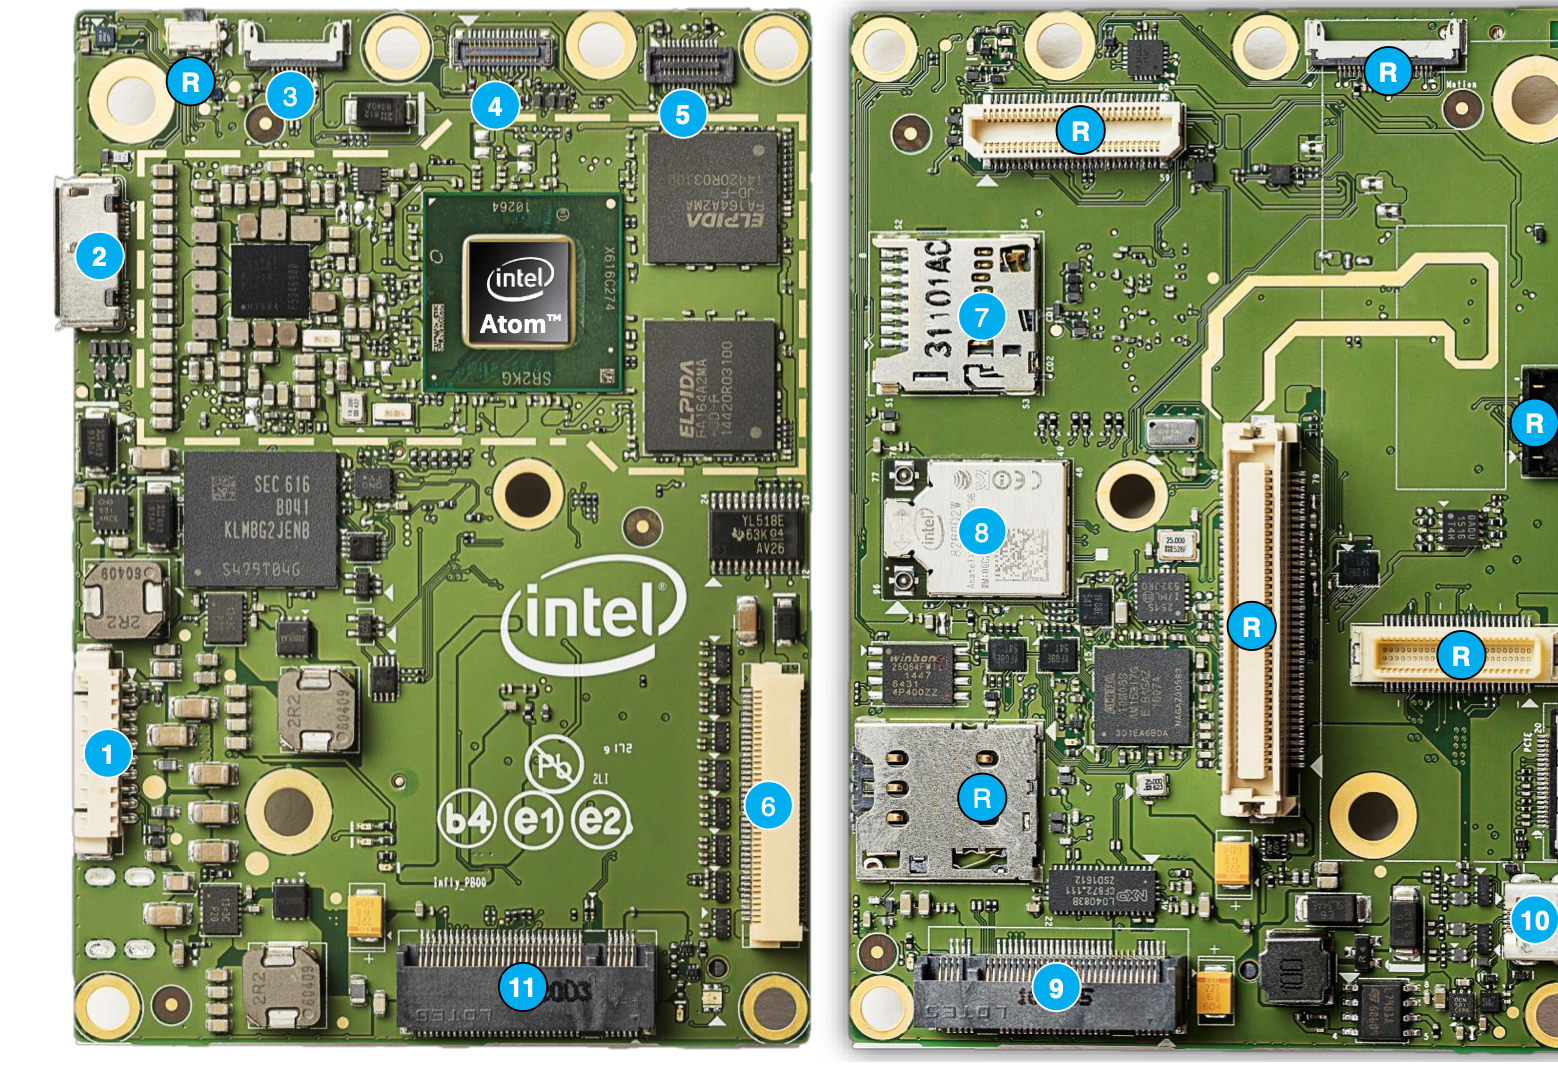
\includegraphics[width=\linewidth]{templates/images/chapter05/intel-aero-compute-board.png}
        \end{minipage}}&1&Power connector\\
        &2&USB 3.0 OTG \\
        &3&Interface for Intel RealSense camera \\
        &4& MIPI interface for HD camera \\
        &5& MIPI interface for VGA camera \\
        &6& 80 pin flexible I/O (I2C,SPI,UART) \\ 
        &7&microSD Memory Card slot\\
        &8&Intel Dual Band Wireless-AC\\
        &9&PCIe x1 M.2 Interface\\
        &10&Micro HDMI port\\
        &11&NGFF M.2 connector\\
        &R&RESERVED for future use\\
        %\cmidrule(r){2-3}%\hline
      \end{tabular}
      \caption{Intel Aero Compute Board Connector Layout. Source: \cite{intel-aero-combrd}}
      \label{tbl:aero-board-layout}
    \end{table}
\newpage 
    All signals from the Aero Flight Controller (except the SDIO interface and CAN bus) are routed through the MAX10 FPGA to the IO Expansion connector. The pin assignments can be found in the Hardware Features and Usage document. The FPGA is in charge of routing the IOs between the (*SoC) System-on-Chip and the motors plus flight controller. The pin functions from the Aero Flight Controller may vary according to the STM32's pinmux configuration. The Flight Controller hardware contains a CAN bus transceiver.
    
    \begin{figure}[H]
        \centering
        \begin{minipage}{0.45\textwidth}
            \centering
            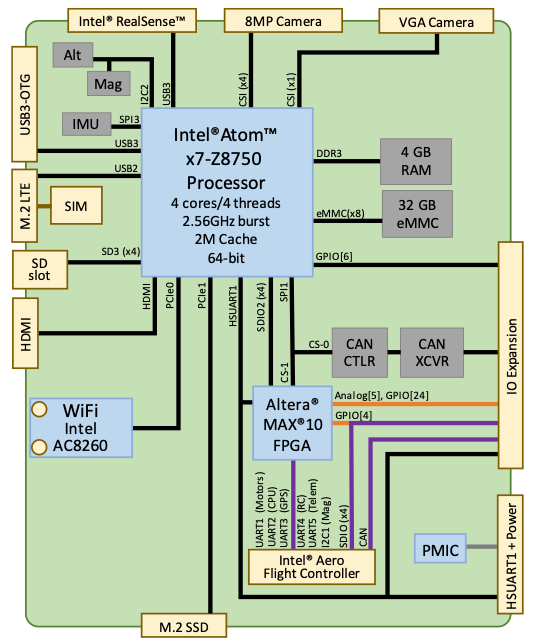
\includegraphics[width=\textwidth]{templates/images/chapter05/compute-board-diagram-nbw.png} % first figure itself
            %\caption{first figure}
        \end{minipage}%\hfill
        \begin{minipage}{0.4\textwidth}
            \centering
            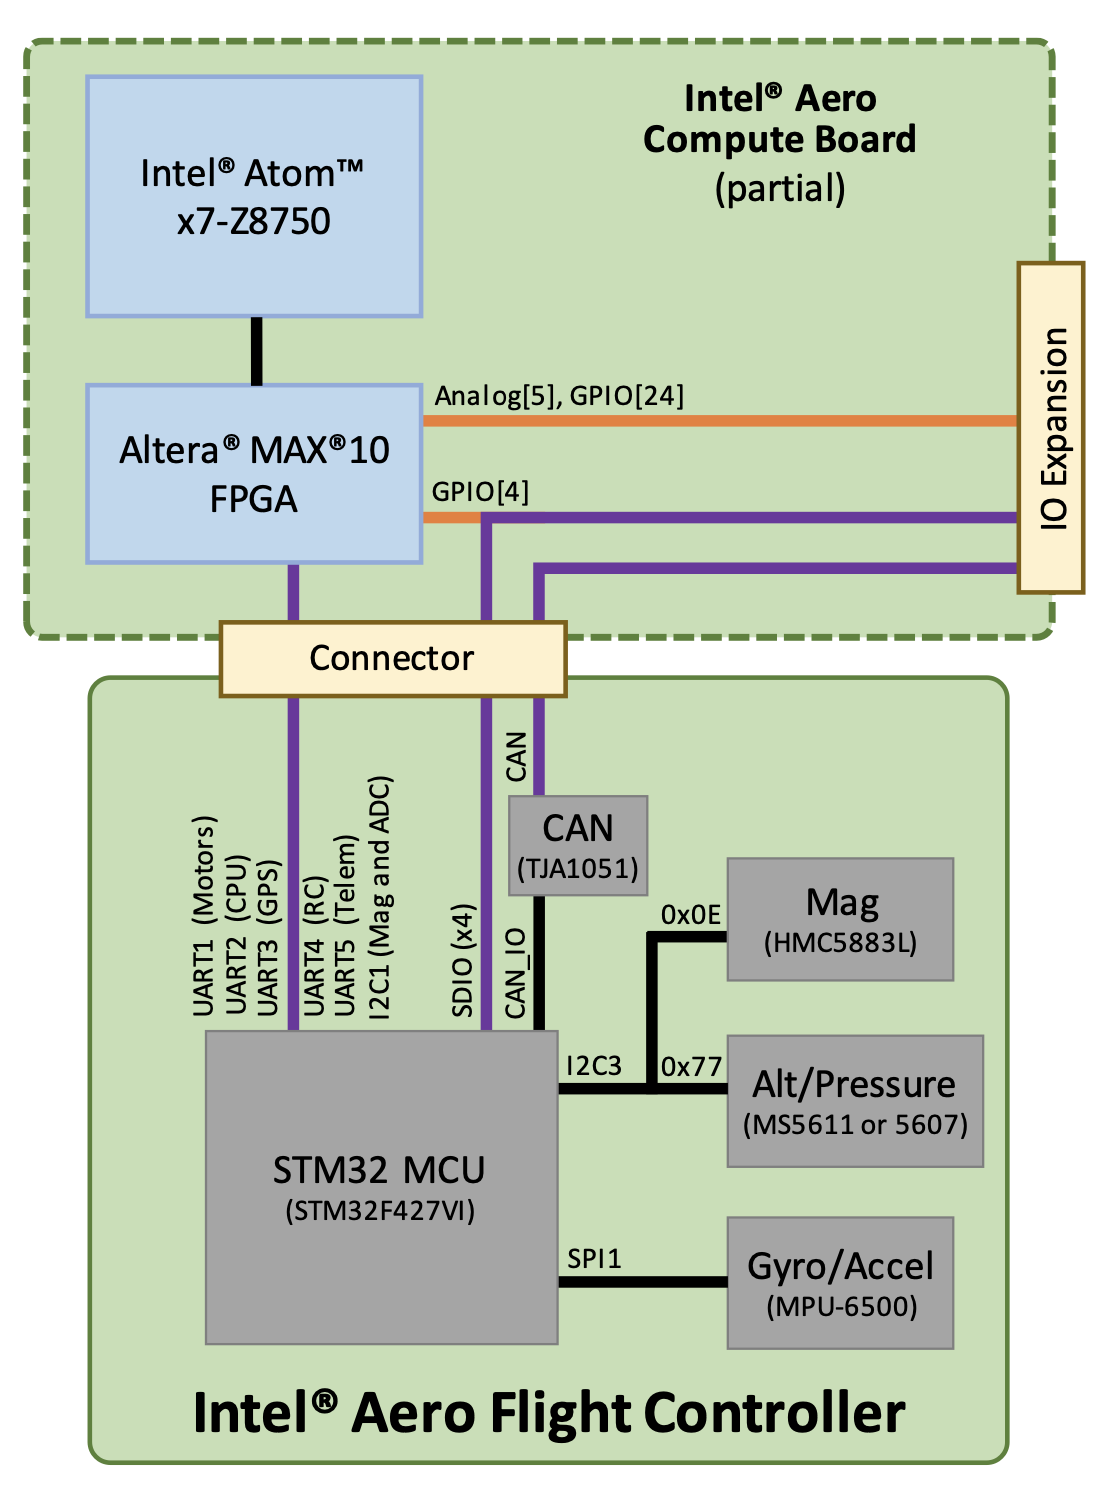
\includegraphics[width=\textwidth]{templates/images/chapter05/flight-controller-diagram-nbw.png} % second figure itself
            %\caption{second figure}
        \end{minipage}
        \caption{Respective module block diagrams. Source: \cite{intel-aero-combrd}}
    \end{figure}
    
    %[*Intel® Aero Compute Board: Hardware Features and Usage Rev 1.5.2,https://www.intel.com/content/dam/support/us/en/documents/drones/development-drones/intel-aero-compute-board-guide.pdf]
\newpage
    By default, Intel Aero board and Intel Aero Ready To Fly kit are delivered with a Yocto Project build already flashed. Yocto project is an open source set of tools for embedded professionals. The UEFI BIOS is maintained by InsydeH20.\footnote{Since September 04, 2019, Intel has discontinued the Intel Aero Platform for UAVs. Forum-based support (Intel Community) for Intel Aero products is available until June 15, 2019. There are no further software updates planned for the Intel Aero Platform for UAVs. All documentation resources for the Intel Aero products will be available to the Intel Aero developer community until February 15, 2022. Files licensed under open source licenses will continue to be available in binary and source code on GitHub.} This Yocto build is preconfigured and highly customized for Intel Aero. In parallel to this Intel supported Yocto image, full native Ubuntu with Intel drivers is available as user installation.
    
    For our use-case a huge effort was dedicated in order to fine-tune the appropriate configuration of hardware and software as to not jeopardize the reliability of the system. More specifically, it was found that under no circumstances any other version of Ubuntu Linux 16.04.3 should not be installed, for the sole reason that the system would cease to boot entirely. Additionally, any updates could cause instabilities, including important security patches. For this reason, the software stack is considered highly insecure in terms of being up-to-date with current Linux distributions and should not be operated on public-facing infrastructures and is intended only for demonstration purposes. 
    
    Facing a choice between the two Linux distributions available for the platform, namely a pre-configured Yocto Project supplied by Intel with the necessary packages for conventional applications or the desktop version of Ubuntu 16.04, versatility was a deciding factor. Although more lightweight and use-case specific, Yocto does not come with a package manager, with the only option being a re-compilation of the system image using so-called "recipes", something that would be extremely time consuming and with varialble results. For this reason, we opted for the commercially available Ubuntu distribution, placing additional care as to not diverge greatly from the basic configuration, apart from necessary packages for our use-case.
    
    \begin{figure}
        \centering
        \begin{minipage}{0.5\textwidth}
            \centering
            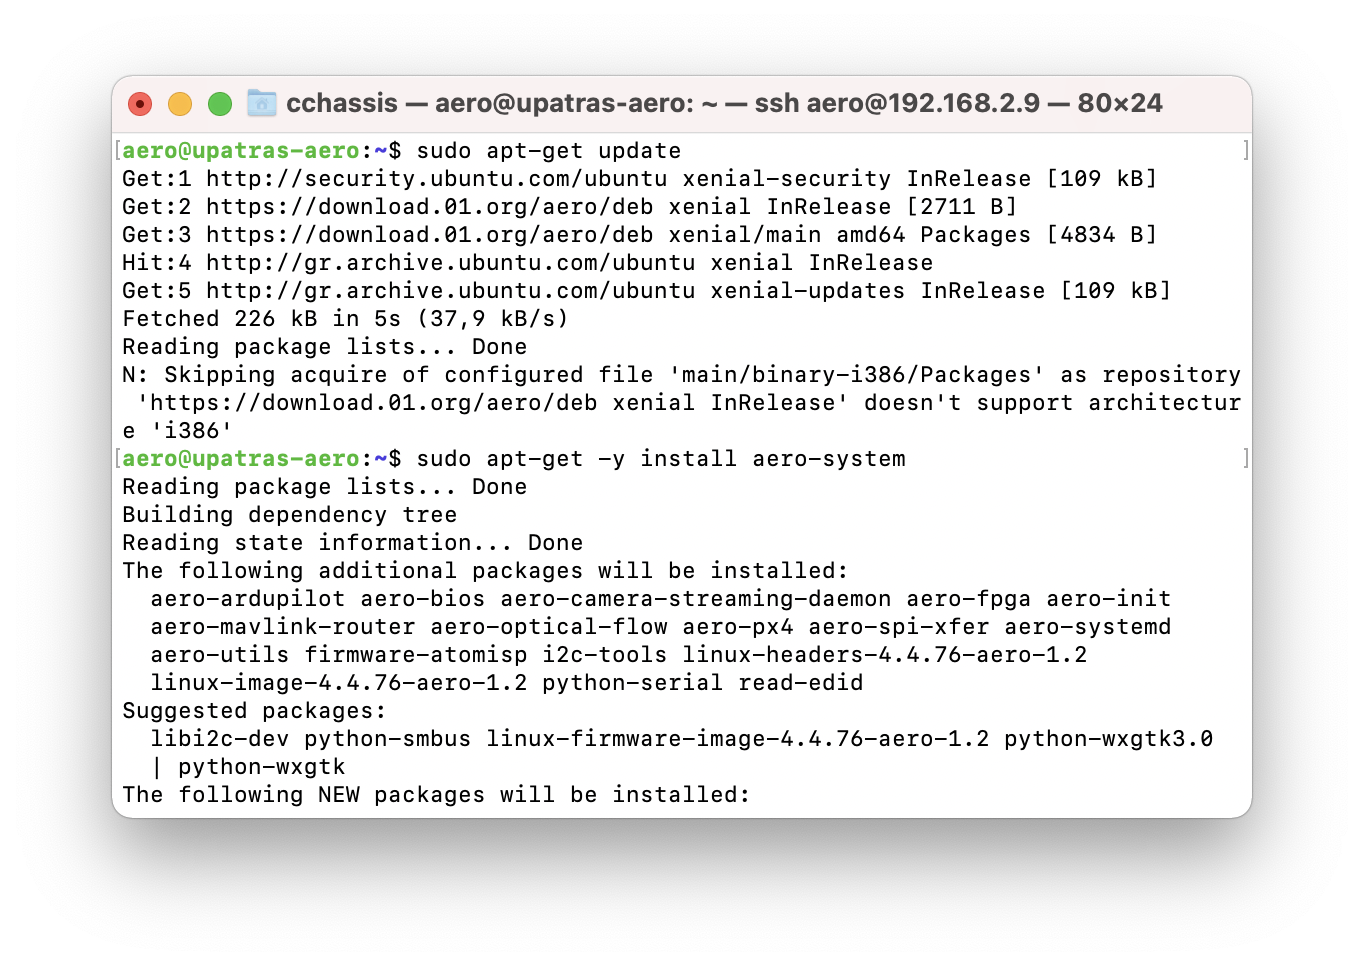
\includegraphics[width=\textwidth]{templates/images/chapter06/06-04-install-aero-system.png} % first figure itself
            %\caption{first figure}
        \end{minipage}\hfill
        \begin{minipage}{0.48\textwidth}
            \centering
            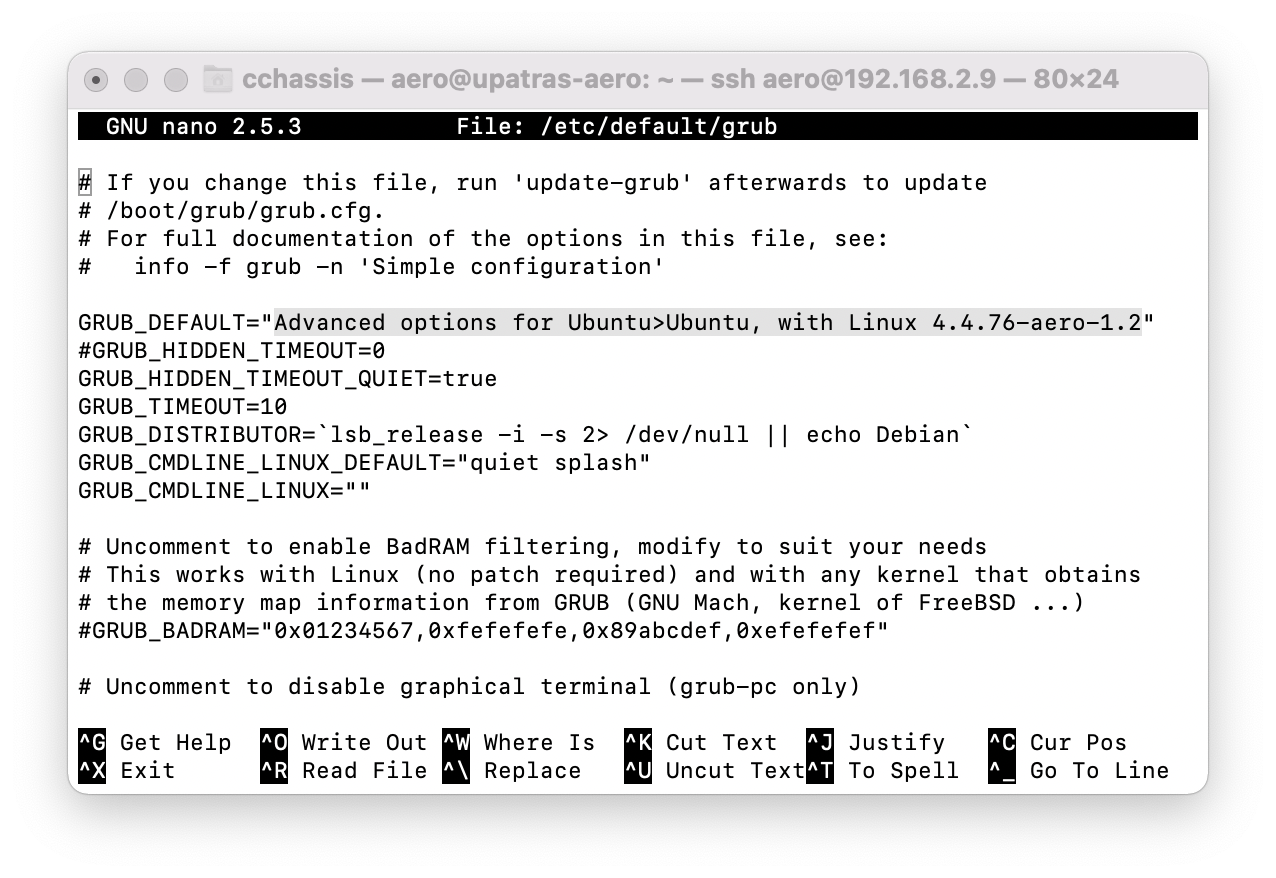
\includegraphics[width=\textwidth]{templates/images/chapter06/06-05-bnw.png} % second figure itself
            %\caption{second figure}
        \end{minipage}
        \caption{Downloading and setting correct kernel version.}
    \end{figure}

    \subsection{Flight Controller}
    Included in the Ready to Fly (RTF) kit, an STM32F427V autopilot board is responsible for hosting the Real Time Operating System (RTOS), under which the Autopilot Software Suite operates. The flight controller also hosts a variety of sensors responsible for vital vehicle operations such as a magnetometer and a compass, along with a plethora of connectivity for additional use-case specific modules. This specific module comes pre-installed on the aformentioned companion computer, attached via a proprietary connector. This raises some questions regarding the serviceability of the platform, since replacement parts are no longer available, but an external aftermarket flight controller can always be connected via a USB connection.
    
    Regarding the autopilot, the two most popular stacks were under consideration for this implementation, namely PX4 and Ardupilot, with the former being the ultimate choice. PX4 consists of two main layers: the flight stack which is an estimation and flight control system, responsible for the basic functionalities of any autonomous vehicle such as balancing and positional awareness and the middleware, which is a general robotics layer that can support any type of autonomous robot that consists primarily of device drivers for embedded sensors and communication with the external world (companion computer, Ground Control Stations, etc.).
    
    \subsection{Cameras}
    Placed in the front-facing side of the quadrotor assembly, the Intel® RealSense™ R200 module is a implements a long range, stereovision 3D imaging system that implements a variety of capabilities to be used accordingly. More specifically, it can provide color, depth, and infrared video streams. Depth video streams are like color video streams, except each pixel has a value representing the distance away from the camera instead of color information. It consists of an infrared laser projection system, two infrared and a full HD color imaging sensors. The depth video stream is generated with stereo vision technology assisted by the Infrared laser projector and the two infrared imaging sensors. Color data is provided by the full HD color imaging sensor.
    
    Due to the complexity of such device, additional effort has to be taken in order to ensure proper operation during the use-case scenario.
    
    Initially, a custom kernel must be booted in order for the various camera modules to be recognized appropriately. Following, the legacy branch of the RealSense R200 public repository must be configured on the Ubuntu 16.04.3 OS, where after successful initialization, three distinct video devices should be listed using the command  \verb|sudo v4l2-ctl --list-devices|.
    To check if the camera drivers are correctly installed, list the video devices with \verb|ls /dev/video*|
%https://github.com/intel-aero/meta-intel-aero/wiki/90-(References)-OS-user-Installation#checks
    
    
    \subsubsection{Third Party Cameras} %any 360 cameras w/ linux drivers?
    It is also possible to connect another camera for further use case expansions. What is imperative though is ensuring compatibility with existing IO ports on the Intel Aero compute board (SPI, CAN and USB are available) and linux driver support (typically UVC, USB Video Class). The camera is recognized as a UVC device, as expected. As before, run \verb|ls /dev/video*| to list the video devices. Use \verb|sudo v4l2-ctl --list-devices| to get the details about the camera-number association.
%https://github.com/intel-aero/meta-intel-aero/wiki/06-Cameras-and-Video#third-party-usb-cameras
    
    %\section{Software}


\newpage

    \subsection{Additional Software}
    
    Following proper setup of both the software and hardware aspects of the system, the next step is to ensure its key functionalities in order to operate within the use-case requirements. For this reason, two main software stacks need to be individually installed and configured, detailed below.
    
    \begin{figure}[H]
        \centering
        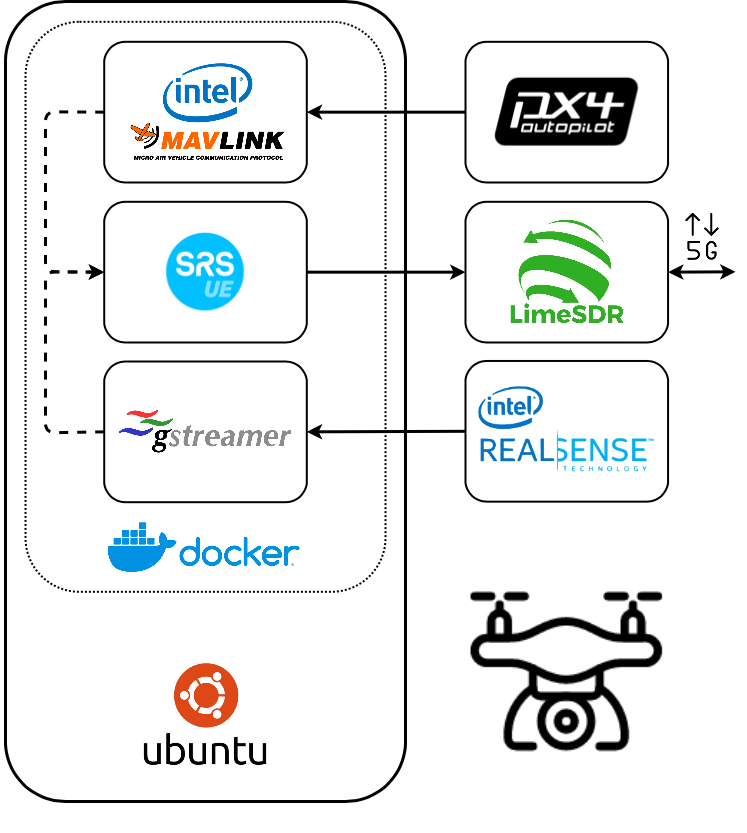
\includegraphics[width=0.9\textwidth]{templates/images/chapter05/vehicle-side-overview-2.png}
        \caption{Vehicle-side overview of the software sub-systems.}
        \label{fig:vehicle-side-sw}
    \end{figure} 
    
    \subsubsection{MAVLink-Router}
    
    MAVLink is a packet implementation for communicating drone messages, a popular interface for flight controllers such as PX4, Ardupilot and more. This was mainly used for Ground Control Stations (GCS) such as QGroundControl and Mission Planner, mainly for the command and control link. MAVLink follows a modern hybrid publish-subscribe and point-to-point design pattern: Data streams are published as topics while configuration sub-protocols such as the mission protocol or parameter protocol are point-to-point with retransmission. MAVLink is a binary telemetry protocol designed for resource-constrained systems and bandwidth-constrained links. The low level implementation of this protocol allows packets to be sent over UDP, TCP and serial interfaces with the exact same message format. Messages can be received over a serial connection and be forwarded to one or many UDP/TCP/serial connections. Telemetry data streams are sent in a multicast design while protocol aspects that change the system configuration and require guaranteed delivery like the mission protocol or parameter protocol are point-to-point with retransmission. Most services use the client-server pattern, such that the GCS (client) initiates a request and the vehicle (server) responds with data. Many existing solutions that provide network routability of MAVLINK packets exist, but the aforementioned MAVProxy, written in Python is relatively slow-performing%[System Engineering and Embedded Software Architecture WOrkshop | UAS@UCLA p.3 of 9 "MAVLink Messages and Routeing (CS118) - https://uasatuca.org/fields/workshops/controls]
    , thus unsuitable for real-time operation. Fortunately, alongside the commercial release of Intel Aero*, the company releaased a plethora of supporting applications, one of which is mavlink-router, written in C++%/ref{*}
    , with its implementation seems more appropriate for low-latency scenarios.
    
    Mavlink-router is an Intel open source project that routes MAVLink streams to specific endpoints, first implemented on the Intel Aero to handle communications with the companion computer. In addition to routing streams, mavlink-router has the ability to route MAVLink streams over a network. This can be done either manually, or through a configuration file.%Using mavlink-router to route MAVLink streams over the network[Jaeyoung Lim-august 25,2018-404warehouse-https://404warehouse.net/2018/08/25/using-mavlink-router-to-route-mavlink-streams/]

\newpage

    \begin{lstlisting}[caption=Example of a typical configuration file.]
[General - Mavlink-router serves on this TCP port]
TcpServerPort=5790
ReportStats=false
MavlinkDialect=auto

[TcpEndpoint Localhost]
Address = 127.0.0.1
Port = 25790
RetryTimeout=10
 
[UdpEndpoint Eavesdropping]
Mode = Eavesdropping
Address = 0.0.0.0
Port = 10000

[UdpEndpoint Endpoint]
Mode = Normal
Address = <ADDRESS>
Port = 11000

[TCPEndpoint LTE]
Address = XX.XX.XX.XX (replace with GCS ip) 
Port = 5760

Log=$HOME/log/flight-stack
LogMode=while_armed
    \end{lstlisting}

\newpage

    Mavlink-router's primary purpose as the name suggests, is to route MAVLink streams between endpoints. The normal usage of mavlink-router is to listen to a flight controller (usually on a serial or UDP port) and forward traffic to other endpoints. A UartEndpoint is defined to listen to a serial device, usually the flight controller. In this case, the flight controller is attached to the ttyS1 serial device of the OS. The mavlink stream can be routed to a UdpEndpoint or a TcpEndpoint of a specified address and port.
    In order to forward streams to Ground Control Stations the parameter \verb|Mode = Normal| needs to be specified. A very important feature is that commands can be sent to the Flight Controller Unit from said endpoints, allowing for complete remote operation over IP. MAVLinks lastly, can be broadcasted over an entire network, by configuring the Bcast address of said network. This proves useful if a VPN (or a network slice) is used as a dedicated network for controlling the drone. \verb|mavlink-router| also listens, by default, on port 5760 for TCP connections. Any connection there will also receive routed packets.

    Lastly, mavlink-router provides logging functions in which enables logging on the companion computer without physically accessing the SD card from the FCU. Logging is simply enabled by adding the Log directory in the configuration file. You can also specify the LogMode in order to set the behavior of the logging. if log mode is set as \verb|LogMode=whlie_armed| the log file is created only once the flight controller is armed and marks the file as read-only.

    \begin{enumerate}
    
    \item Route MAVLink packets between endpoints
    The usual configuration is to have one "master" endpoint that is the flight stack (either on UART or UDP) and other components that can be on UDP or TCP or UART endpoints. This is not strictly required and other configurations are possible: mavlink-router mainly routes mavlink packets from one endpoint to the other endpoints without differentiating what they are.
    
    \item Multicast MAVLink packets to UDP endpoints
    \begin{lstlisting}
$ mavlink-routerd -e 192.168.7.1:14550 \
  -e 127.0.0.1:14550 /dev/ttyS1:1500000
    \end{lstlisting}
    
    \item Route mavlinks packets from any interface (localhost)
    The mavlink-router can be used to route packets from localhost to an external interface. To route packets between SITL running on one computer (sending MAVLink traffic to localhost on UDP port 14550), and QGC running on another computer (e.g. at address 10.73.41.30) you could:
    \verb|$mavlink-routerd -e 10.73.41.30:14550 127.0.0.1:14550|
  
    \item Test mavlink-router 
    By using examples/sender.py and examples/receiver.py to simulate traffic of mavlink messages. First script sends mavlink ping messages to a target mavlink system-id, and second receives and responds to them.
    \verb|$ python examples/sender.py 127.0.0.1:3000 100 0|
    Will send mavlink pings to UDP port 3000. Those pings will have 100 as source system id and will have 0 as target system id (0 means broadcast). Receiver could be set as:
    \verb|$ python examples/receiver.py 127.0.0.1:4000 50|
    Where 50 is the receiver system id. Then, to route between those:
    
    \verb|$ mavlink-routerd -e 127.0.0.1:4000 0.0.0.0:3000|
    Note that it's possible to setup multiple senders and receivers to see mavlink-router in action.
    %[https://github.com/intel/mavlink-router]
    
    \item Enable MAV\_BROADCAST
    By enabling MAV\_BROADCAST, heartbeats are periodically sent out on the local network. A remote computer can then connect by listening to the appropriate port (i.e. 14550 for QGroundControl).
    %https://dev.px4.io/v1.9.0/en/middleware/modules_communication.html
    
    \item Route packets from Localhost
    
    %[https://dev.px4.io/master/en/simulation/#default-px4-mavlink-udp-ports]
    \end{enumerate}
    
    After saving, restarting the router service is required with \verb|sudo systemctl restart mavlink-router|. Launching QGroundControl on the user side should automatically receive telemetry feed from the drone.
    
\newpage
    
    \begin{figure}[H]
    \centering
            \begin{minipage}{0.7\textwidth}
            \centering
            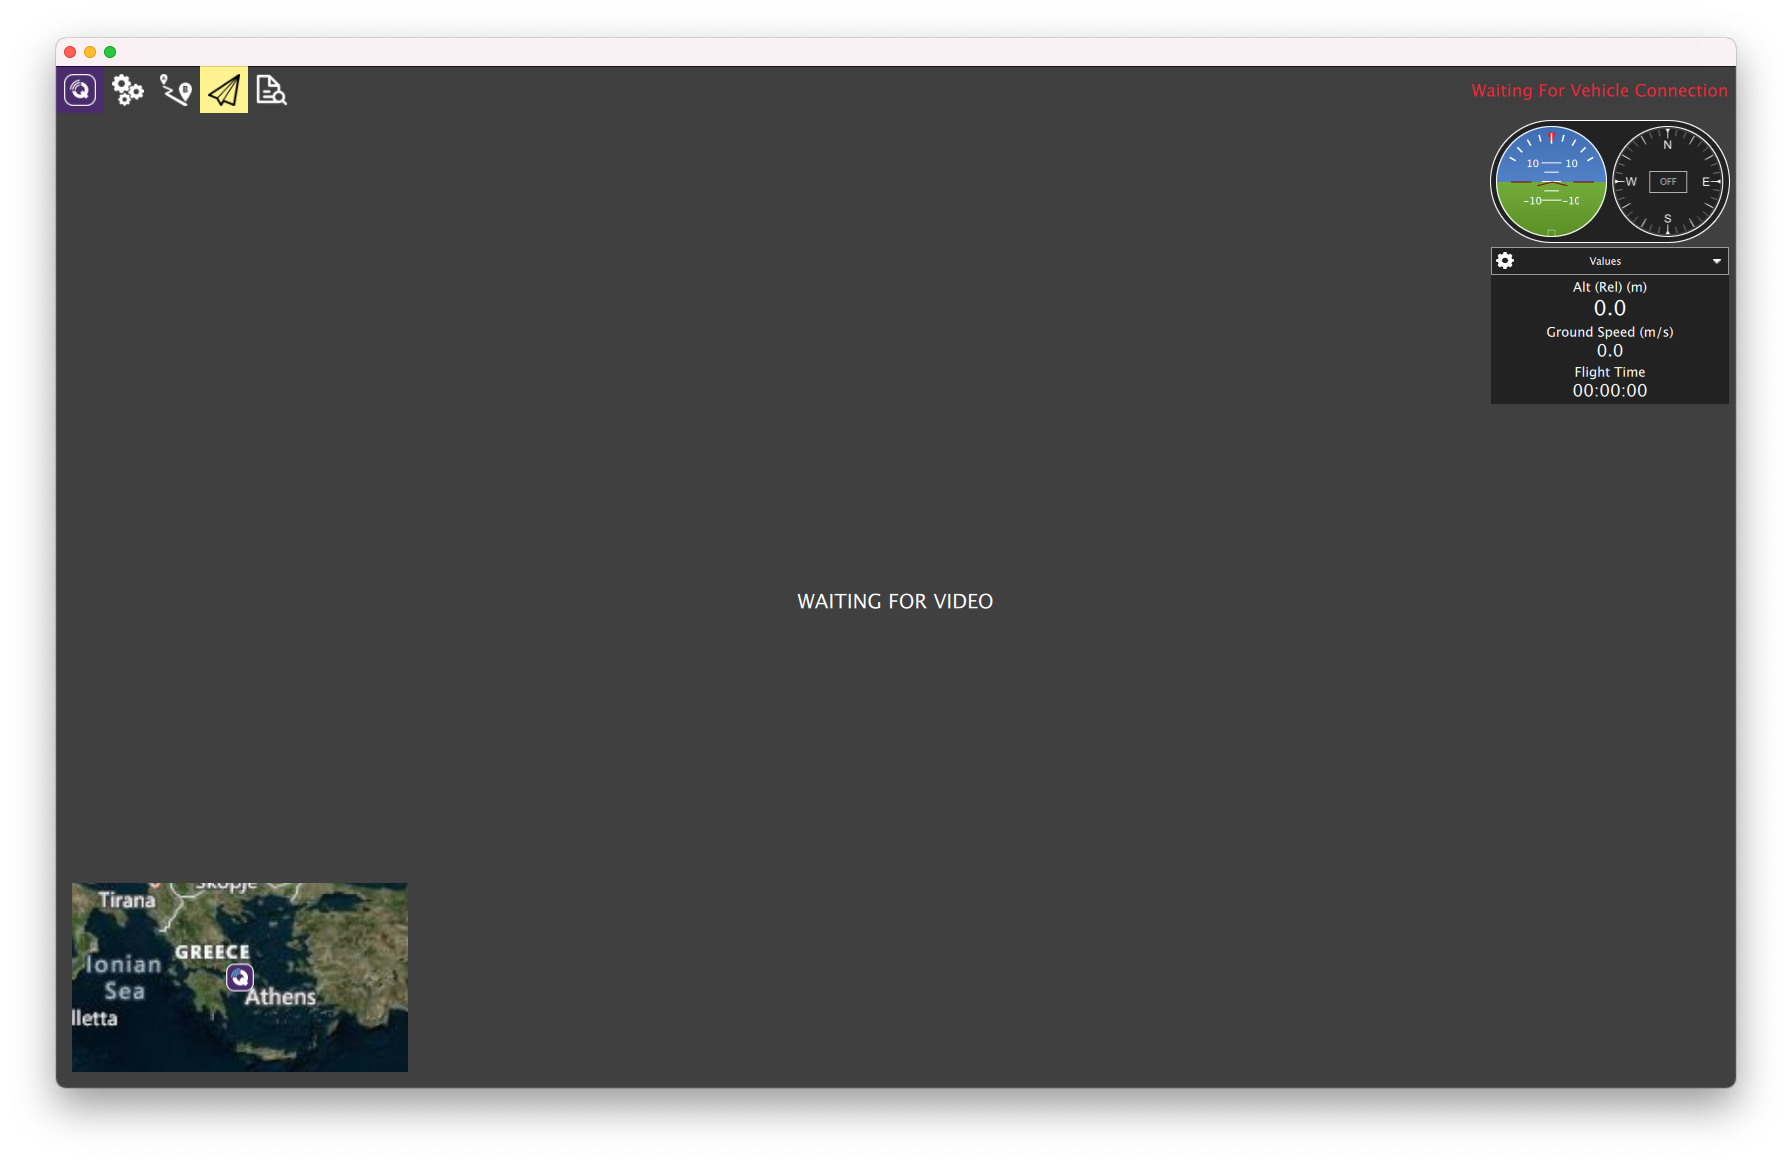
\includegraphics[width=1\textwidth]{templates/images/chapter05/qgc-before.png}
        \caption{Default Ground Control Station software state.}[Bottom row displays the request to allow traffic through the MAVLink port and the resulting information.]
        \end{minipage}
        
        \begin{minipage}{0.3\textwidth}
            \centering
            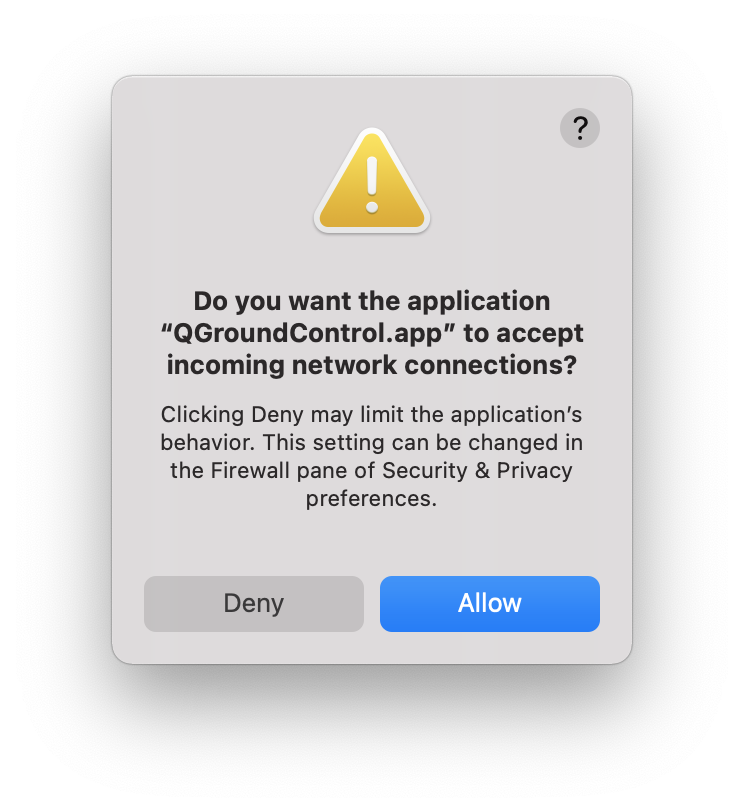
\includegraphics[width=\textwidth]{templates/images/chapter05/open-port.png} % first figure itself
            %\caption{Establish connection through the MAVLink protocol.}
        \end{minipage}\hfill
        \begin{minipage}{0.7\textwidth}
            \centering
            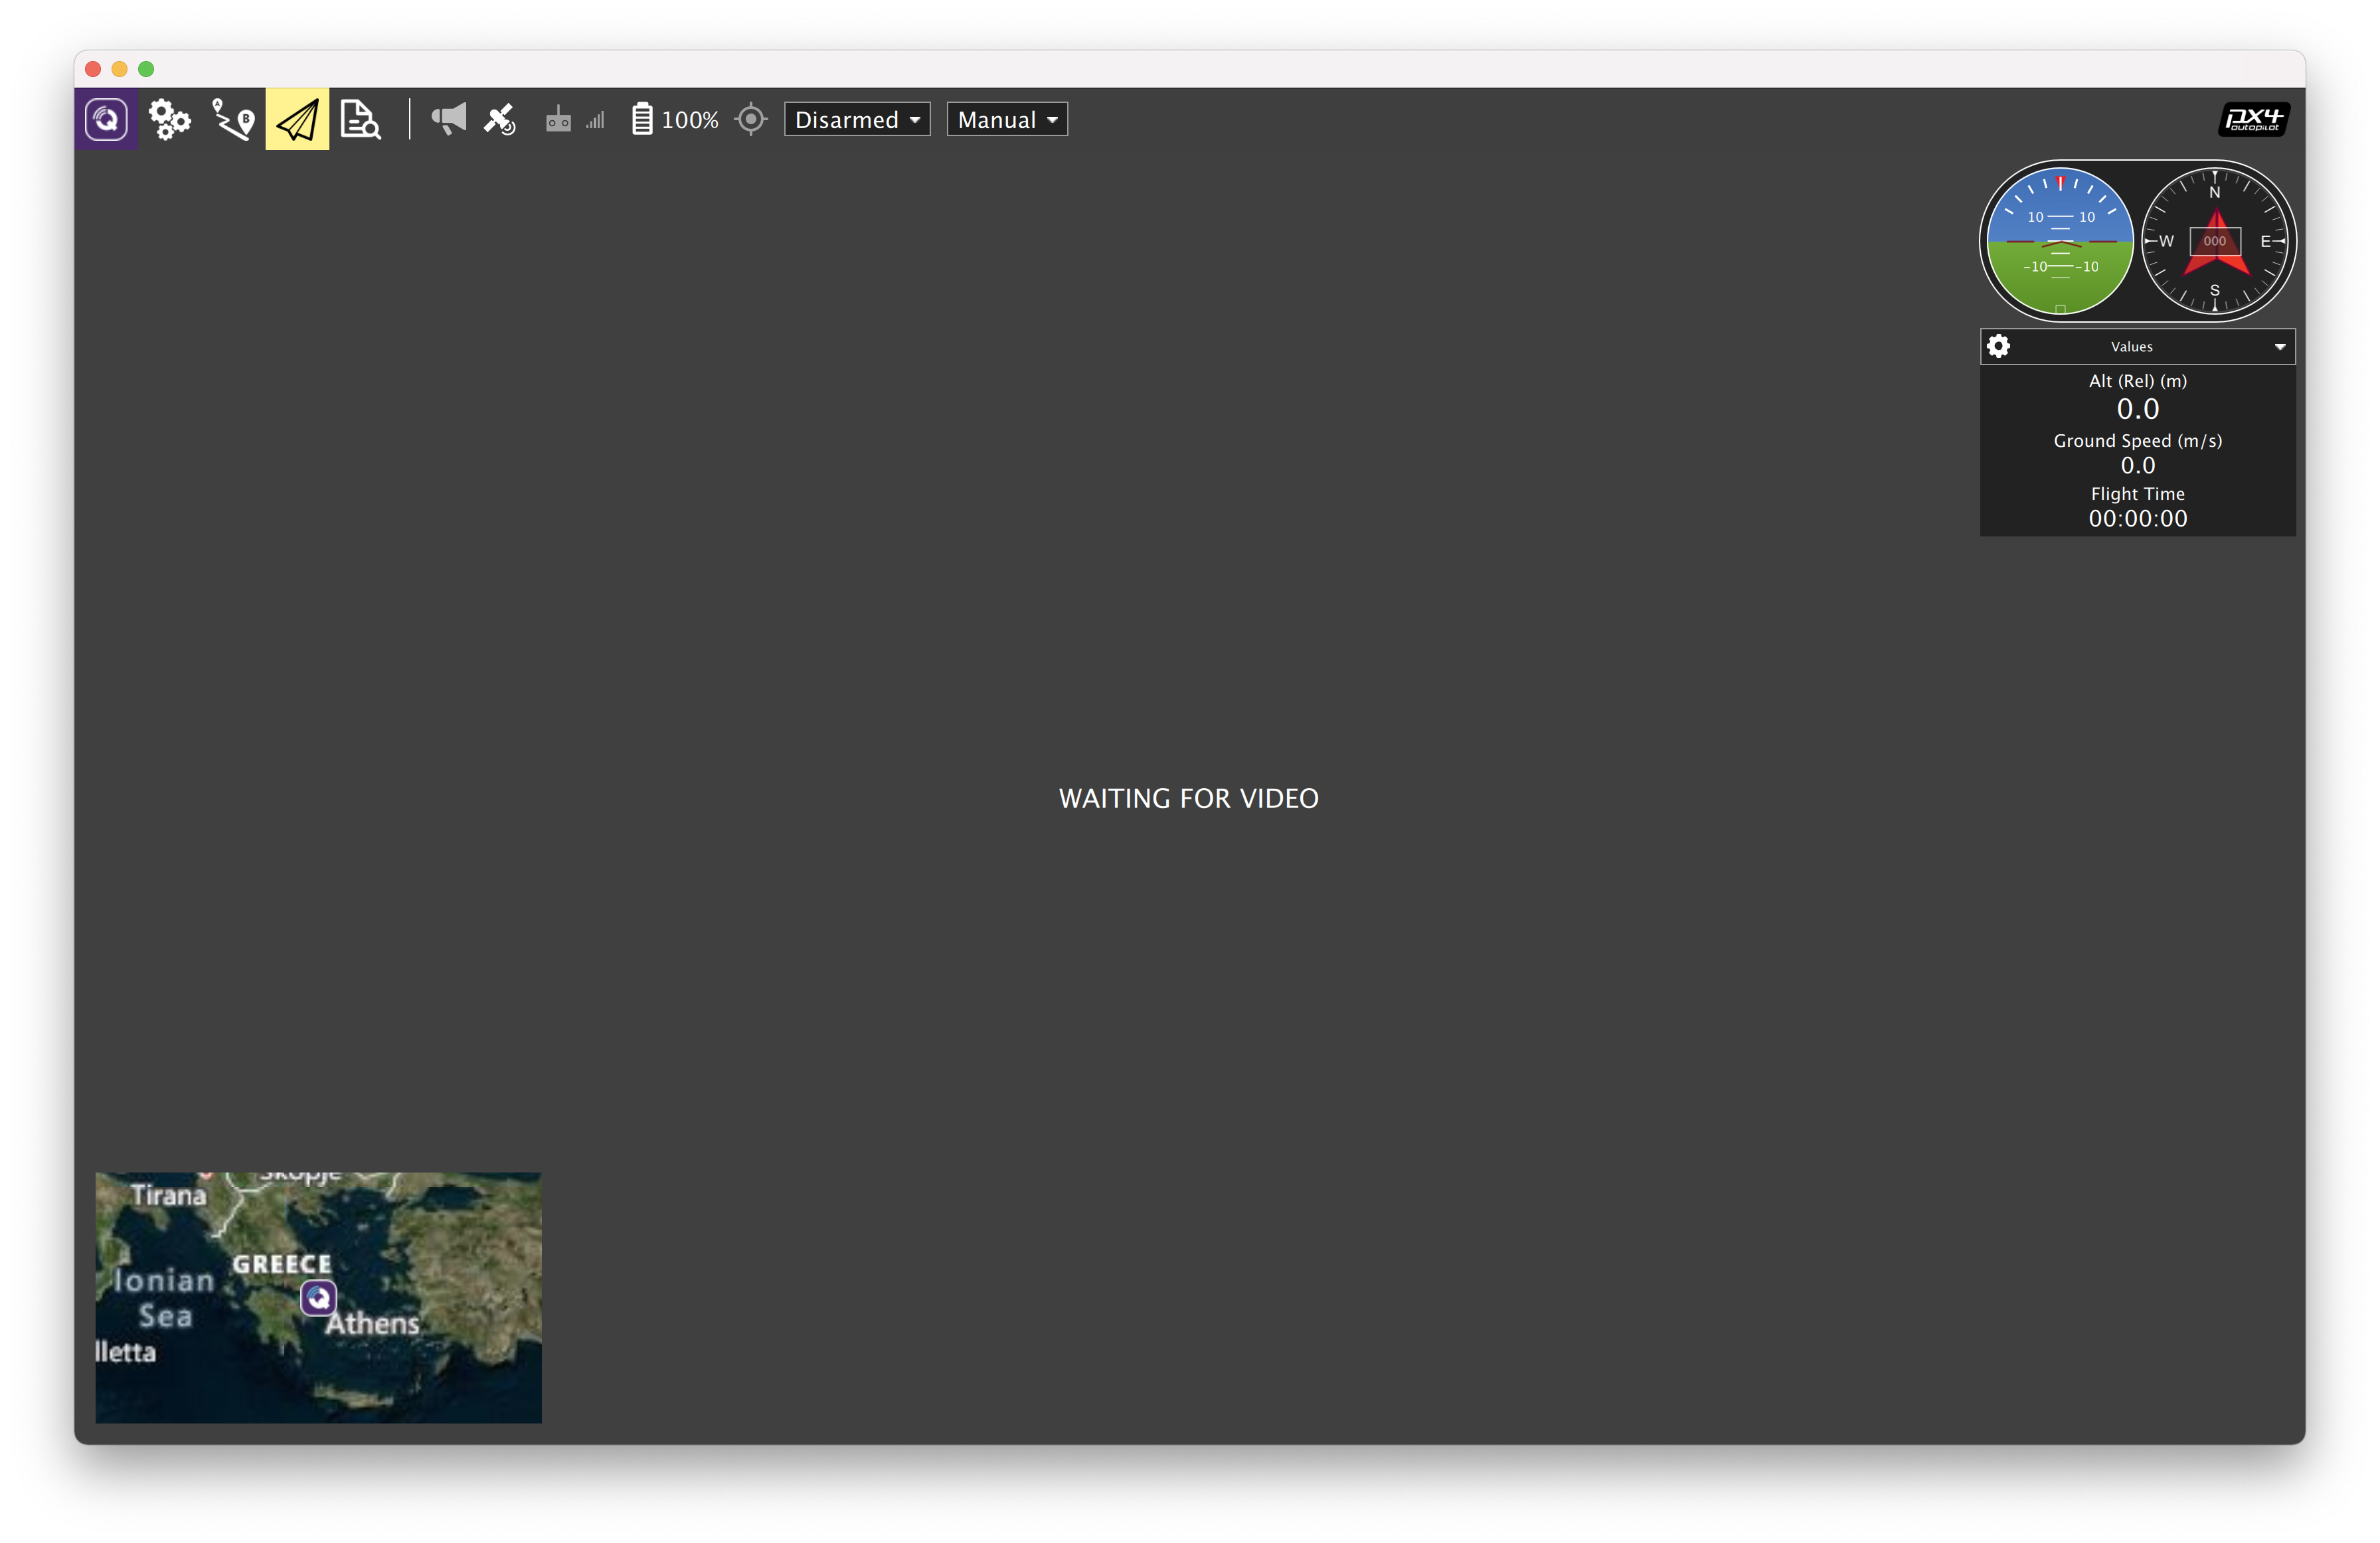
\includegraphics[width=\textwidth]{templates/images/chapter05/waiting-for-video.png} % second figure itself
            %\caption{Autopilot flight stack successfully connected.}
        \end{minipage}
        %\caption{Ground Station perspective after successful network connection.}
    \end{figure}
    
\newpage
    
    \subsubsection{Intel Camera Streaming Daemon}

    Camera streaming daemon gets installed with aero-system by default. It is responsible for detecting installed camera devices and proposing RTSP feeds. No further manual configuration is required.

    \begin{lstlisting}[caption=Check that CSD is running][H]
$systemctl status csd
csd.service - Camera Streaming Daemon
Loaded: loaded (/lib/systemd/system/csd.service; disabled; vendor preset: enabled)
Active: active (running) <output ommited>
    \end{lstlisting}
    
     Camera Streaming Daemon will stream the video feeds over the network with RTSP, a standard protocol. RTSP video can be received by QGroundControl and typical video players on most platforms.
    
    Intel Aero is proposing by default 5 RTSP video feeds:
    \begin{lstlisting}
RealSense R200, HD camera: rtsp://192.168.8.1:8554/video13
RealSense R200, depth sensor: rtsp://192.168.8.1:8554/rsdepth
RealSense R200, infrared first camera: rtsp://192.168.8.1:8554/rsir
RealSense R200, infrared second camera: rtsp://192.168.8.1:8554/rsir2
Bottom facing global shutter: rtsp://192.168.8.1:8554/bottom
    \end{lstlisting}
    
        \begin{figure}[!ht]
            \centering
            \includegraphics[width=0.4\textwidth]{templates/images/chapter05/rtsp-stream.png}
            \caption{RTSP video stream of the front-facing camera.}
            \label{fig:board-diagram}
        \end{figure} 
    
%    \subsubsection{gstreamer}
%        We covered the Camera Streaming Daemon to stream RTSP feeds. But you can also use gstreamer directly to encode (using the GPU) and send video over the network, drastically improving video latency over VLC. 
%<*own example>
%        Here an example using Yocto, launching a gstreamer command to get video from the RGB sensor of the R200 camera (/dev/video13), select a VGA resolution at 15fps, use the hardware accelerated h264 encoder and send it to a specific IP address:
%       \begin{lstlisting}
%sudo gst-launch-1.0 v4l2src  device=/dev/video13 do-timestamp=true ! video/x-raw, format=YUY2, width=640, height=480, framerate=15/1 ! autovideoconvert ! vaapih264enc ! rtph264pay !  udpsink host=192.168.1.147 port=5600
%        \end{lstlisting}

\newpage 
    \begin{figure}[H]
        \centering
        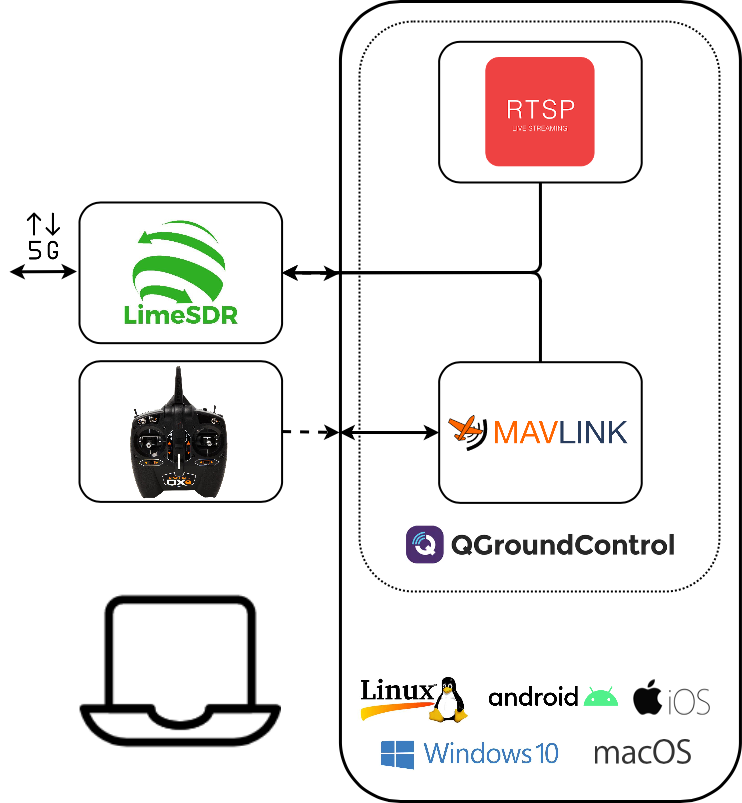
\includegraphics[width=0.9\textwidth]{templates/images/chapter05/user-side-overview-3.png}
        \caption{User-side overview of the software sub-systems.}
        \label{fig:board-diagram}
    \end{figure} 

        \subsubsection{QGroundControl}
        QGroundControl provides full flight control and vehicle setup for PX4 or ArduPilot powered vehicles. It provides easy and straightforward usage for beginners, while still delivering high end feature support for experienced users. The MAVLink "microservices" define higher-level protocols that MAVLink systems can adopt in order to better inter-operateand are used to exchange many types of data, including: parameters, missions, trajectories, images and other files.

        \begin{figure}[H]
            \centering
            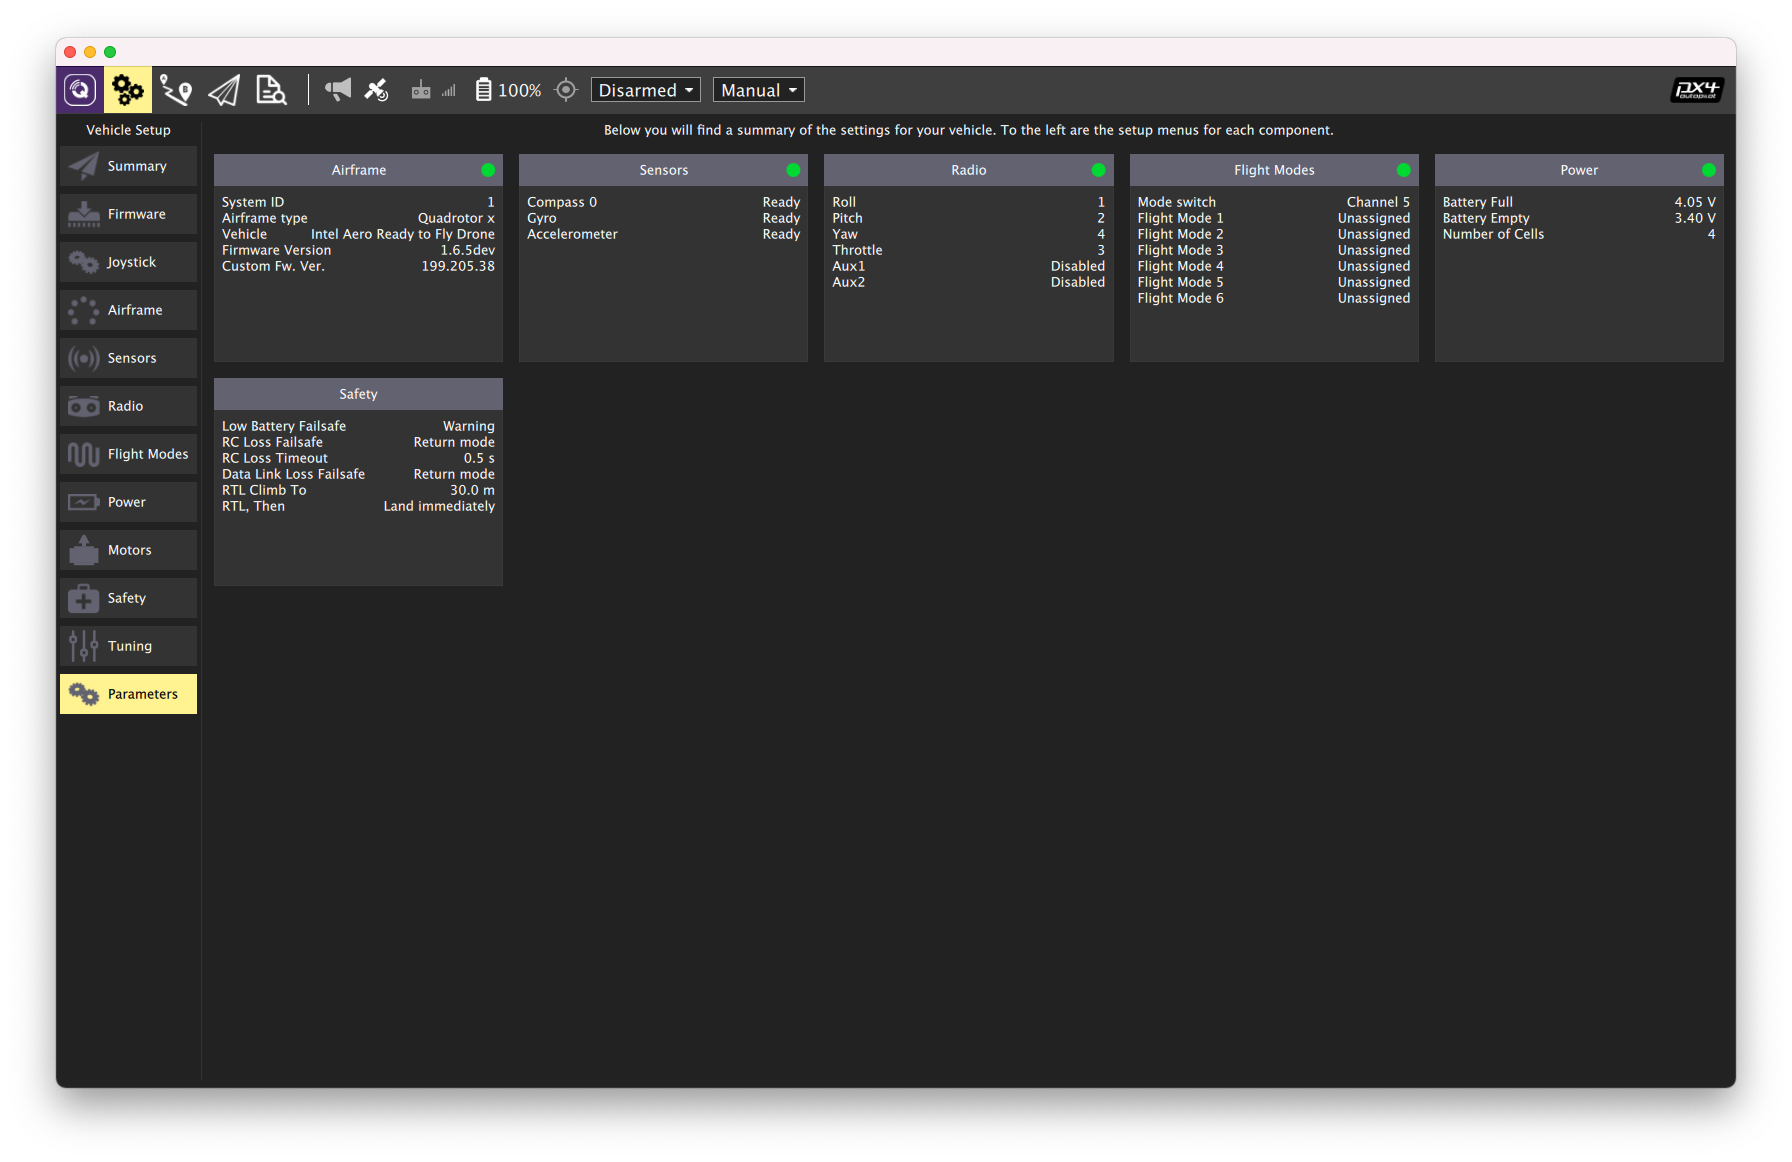
\includegraphics[width=0.9\textwidth]{templates/images/chapter05/passing-all-checks-to-arm-motors.png}
            \caption{Result of proper calibration of all sensors to arm motors.}
            \label{fig:board-diagram}
        \end{figure} 
        
        \begin{figure}[H]
            \centering
            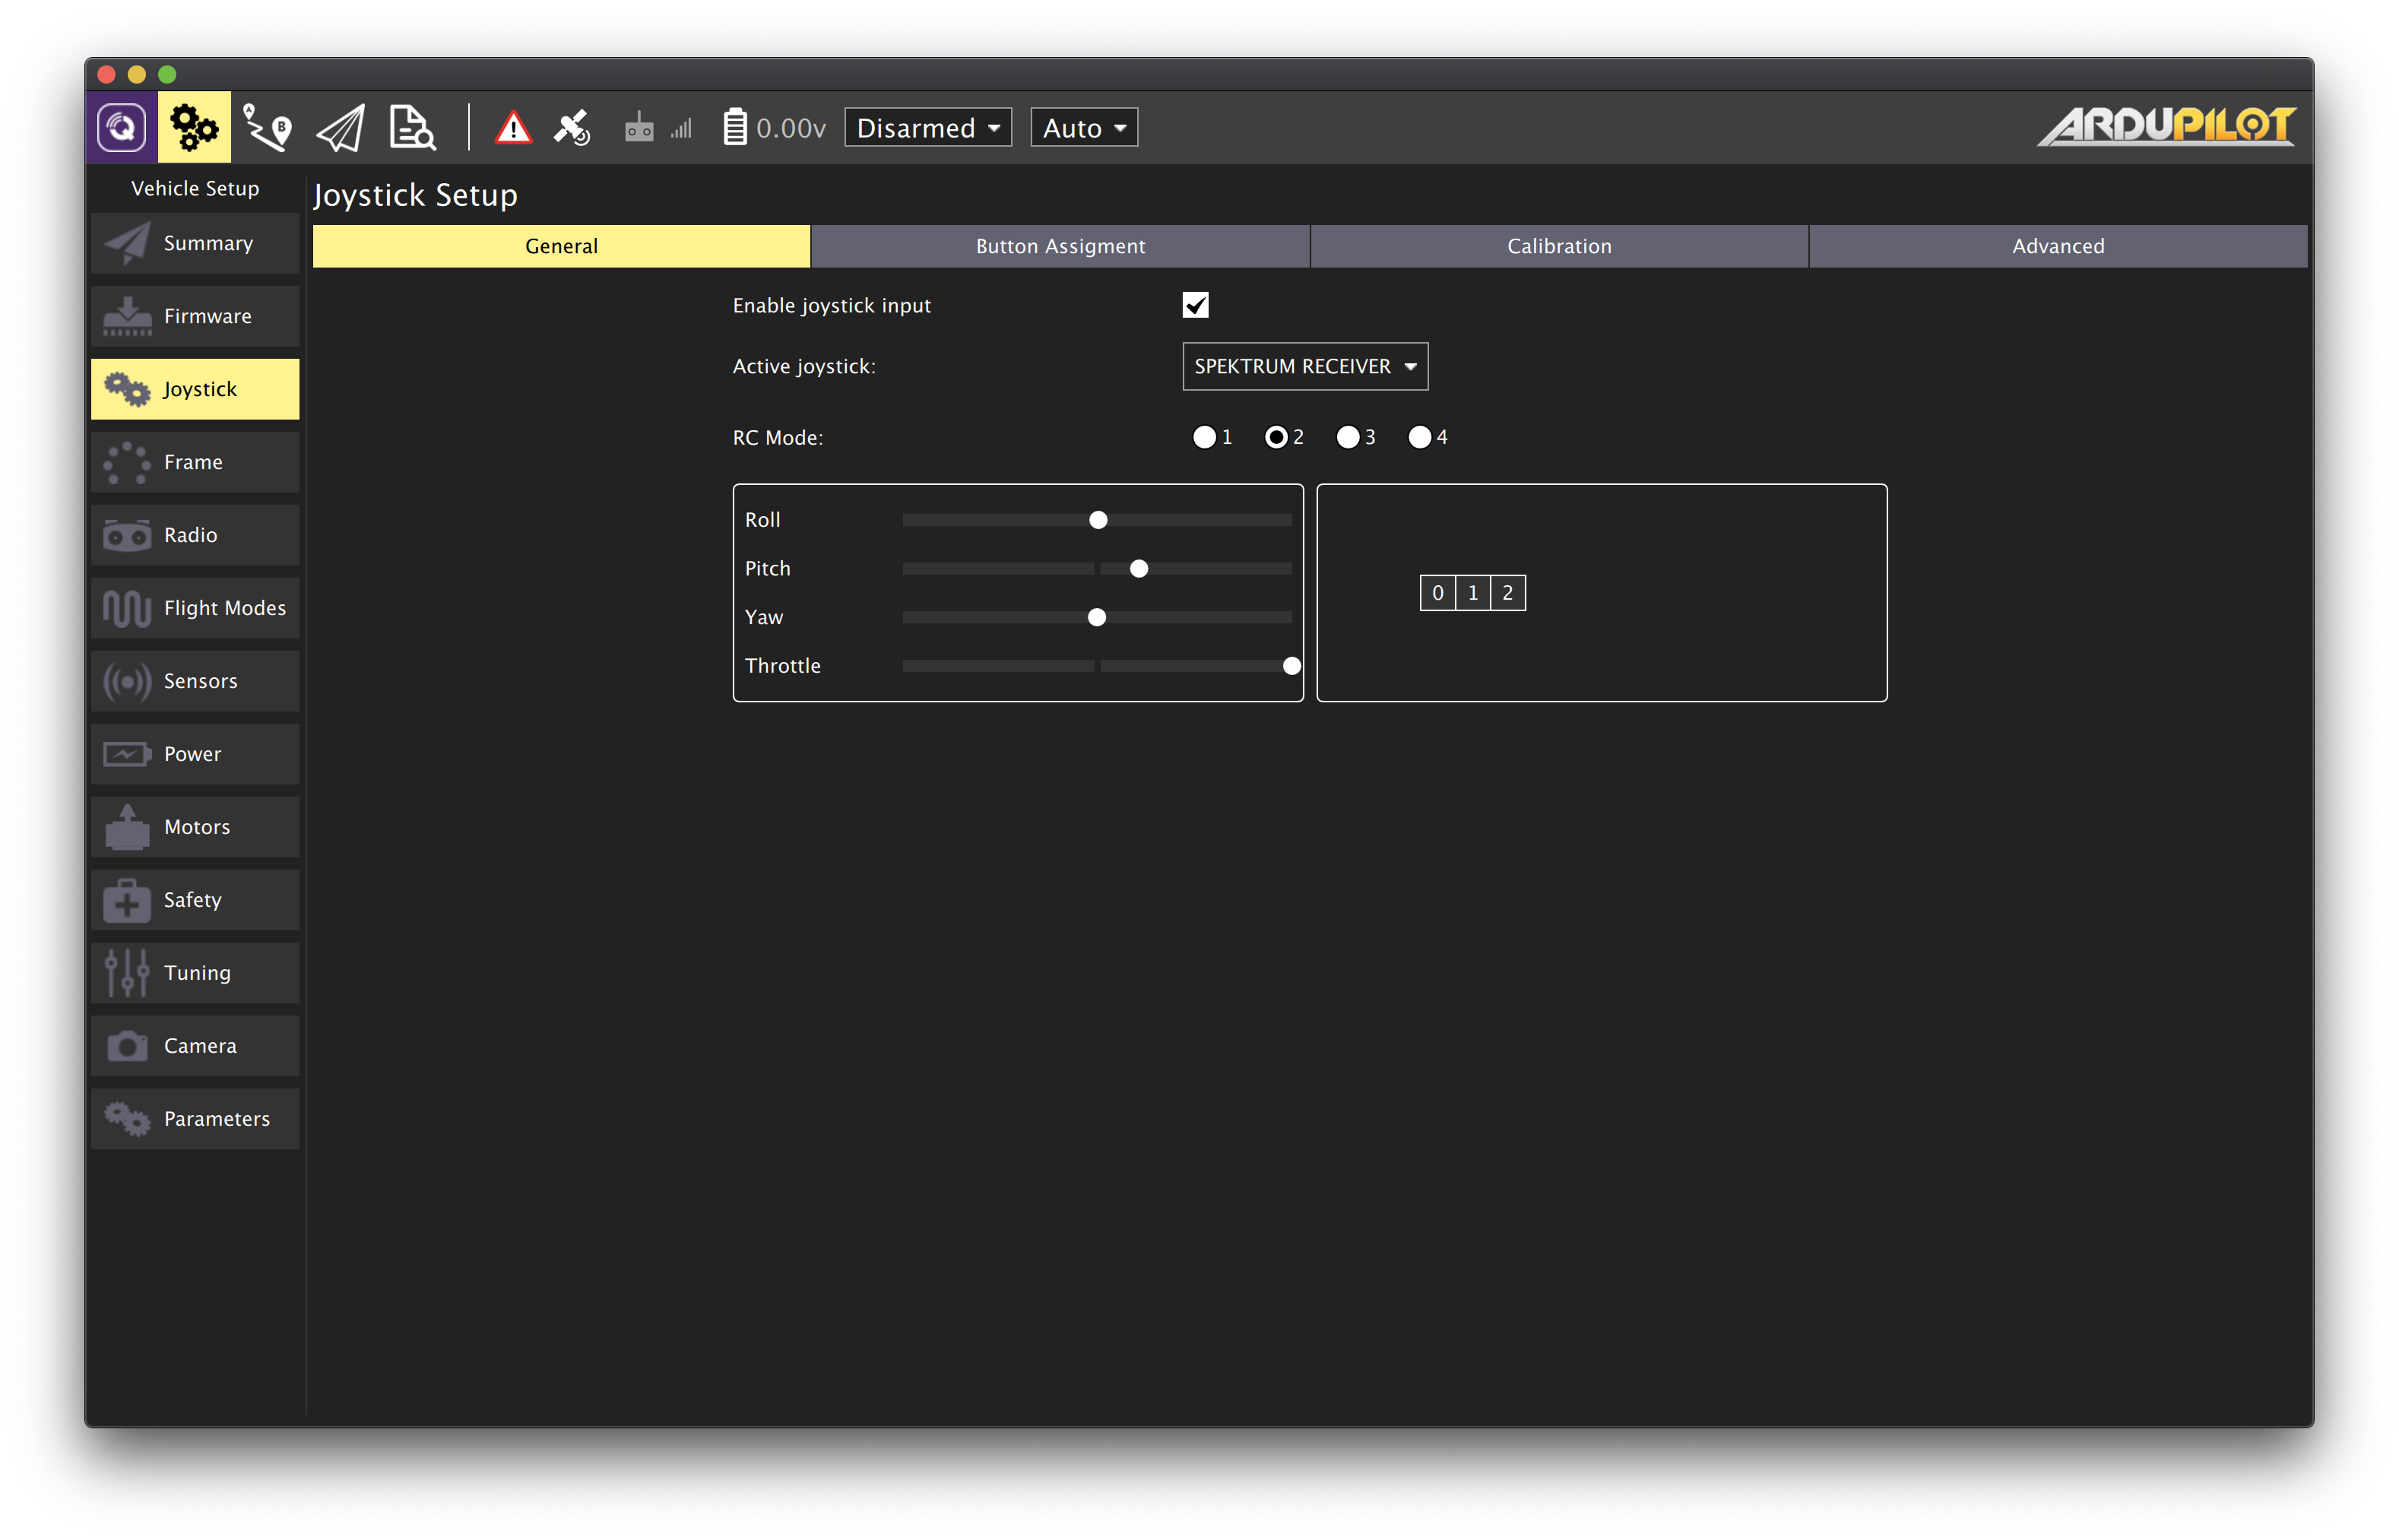
\includegraphics[width=0.9\textwidth]{templates/images/chapter05/joystick-setup-general.png}
            \caption{Verifying wireless controller adapter is recognized as input.}
            \label{fig:board-diagram}
        \end{figure} 
        
        \begin{figure}[H]
            \centering
            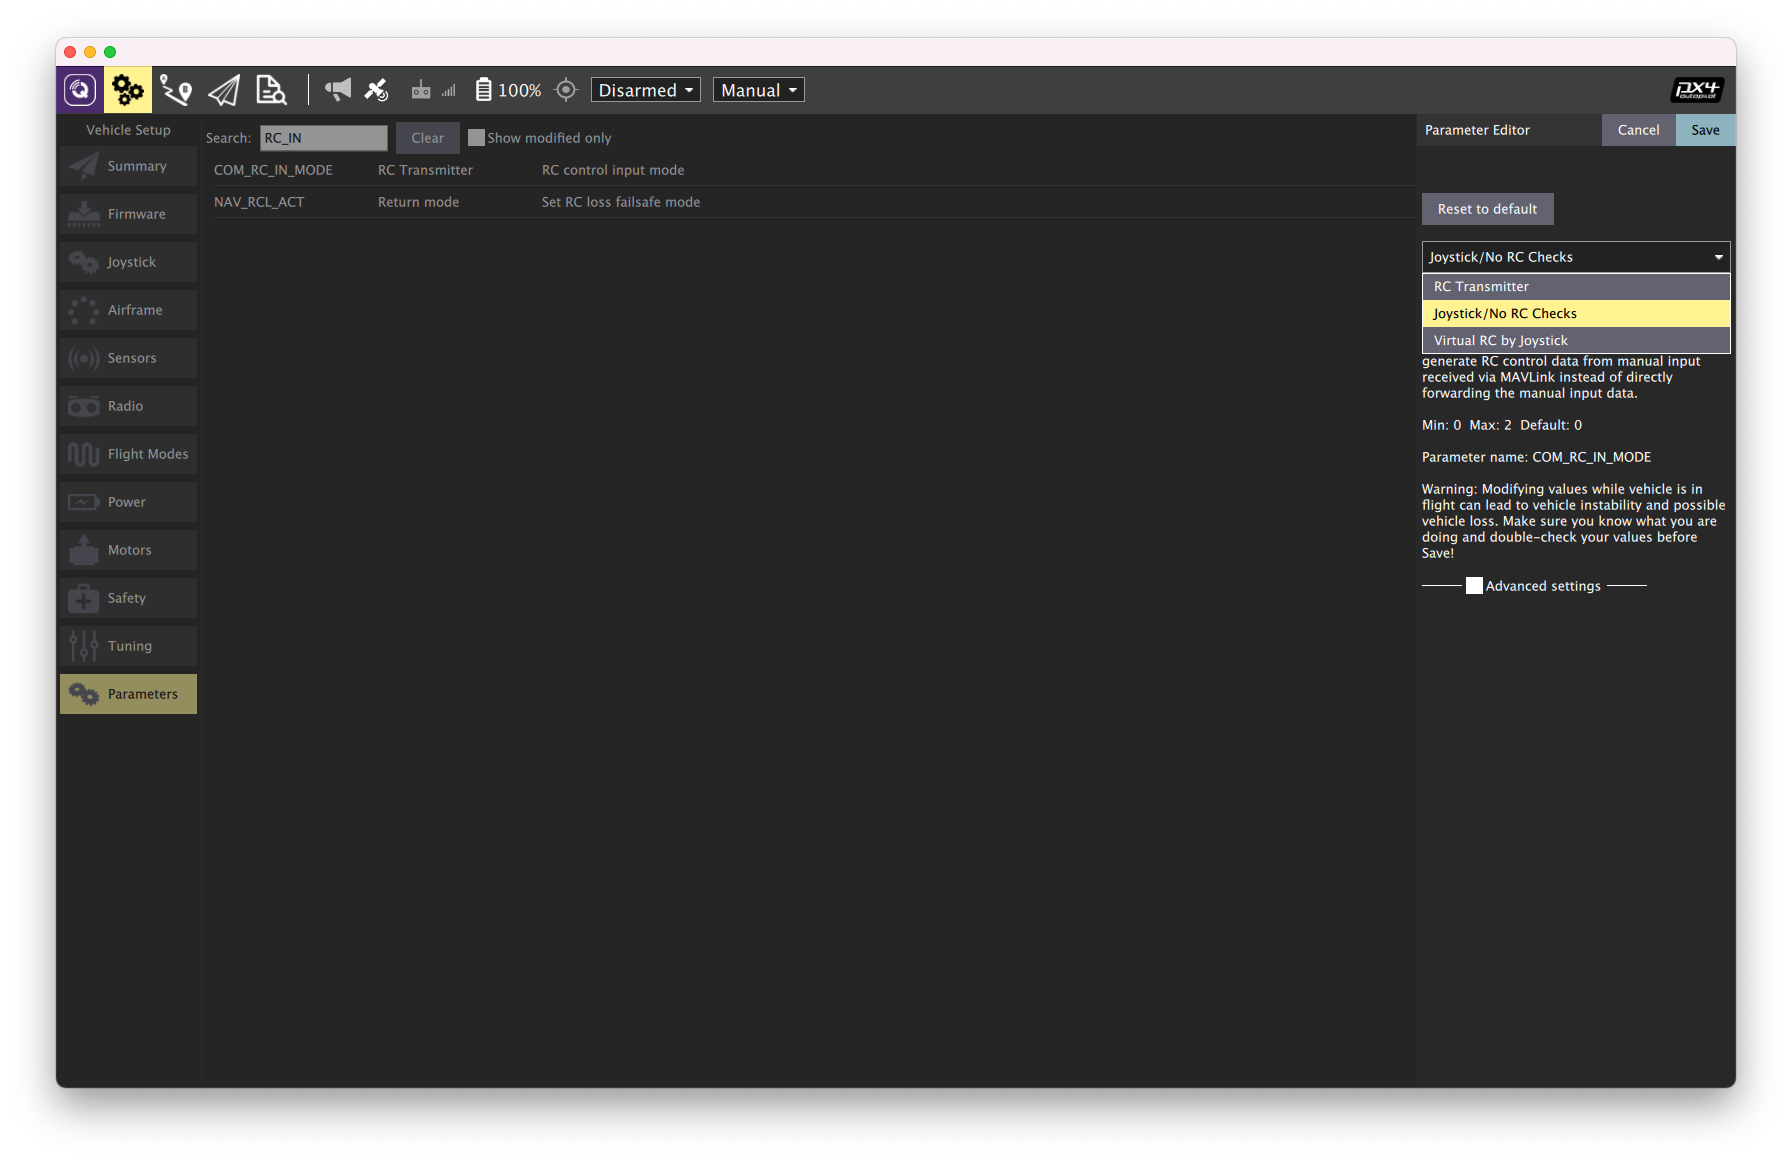
\includegraphics[width=0.9\textwidth]{templates/images/chapter05/setting-joystick-as-input.png}
            \caption{Setting parameter COM\_RC\_IN\_MODE to accept Joystick input.}
            \label{fig:board-diagram}
        \end{figure}
%\newpage
        By default, QGC communicates directly with Aero when connected to the same subnet. However, when the drone is on a cellular connection, a direct connection is non-trivial as both the drone and PC can be behind multiple layers of NATs/firewall. In the options described below, a cloud server is used to help route packets between the drone and PC. Alternatively, the prospective MEC of the gNodeB would be a prime candidate for hosting said instances for greatly reduced latency, as seen on Figure \ref{fig:mav-router}. %MEC of the facility

        On the Intel Aero Ready to Fly Drone (aka Aero RTF), mavlink-router runs locally to handle routing packets between the flight controller and different IP endpoints. But we can also deploy another instance of mavlink-router in the cloud to handle routing just IP traffic. Both the drone and QGC are then connected to this cloud based mavlink-router and communication is established. One benefit of using this method is flight logs are stored automatically in the cloud, so a copy of the logs can always be retrieved. This method also scales well with one-to-many use cases.
        
        \begin{figure}[H]
            \centering
            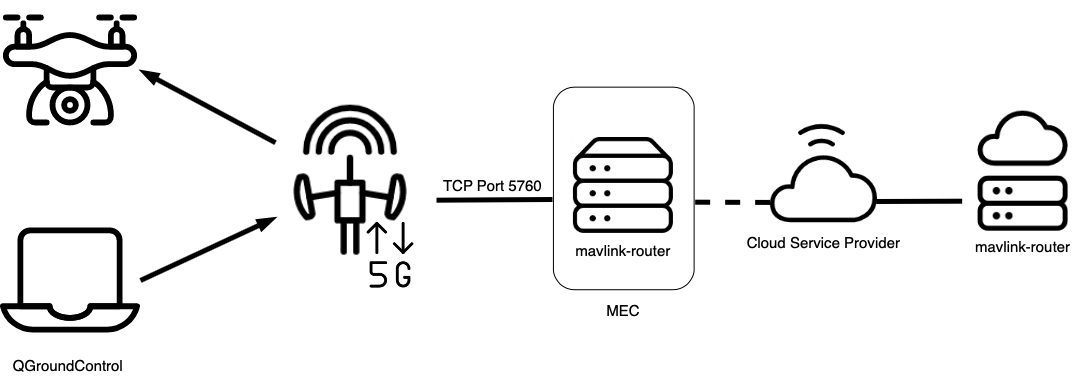
\includegraphics[width=0.9\textwidth]{templates/images/chapter05/mavlink-router.png}
            \caption{MAVLink Router implementation}
            \label{fig:mav-router}
        \end{figure}
%https://github.com/intel-aero/meta-intel-aero/wiki/91-(References)-LTE-Modems#qgroundcontrol-over-lte

        \begin{lstlisting}[caption=Check that MAVLink Router is running]
#Check if the system is listening for MAVLink messages on port 5760:
$netstat -l|grep 5760|
tcp        0      0 *:5760              *:*           LISTEN
        \end{lstlisting}
        
            \begin{figure}[!ht]
                \centering
                \includegraphics[width=0.9\textwidth]{templates/images/chapter05/final-look-QGC.png}
                \caption{Complete view of the Ground Control Station software.}
                \label{fig:board-diagram}
            \end{figure} 
    
\section{Networking}
%    \subsection{WiFi}
    By default, Intel Aero is networking through WiFi, either as a client or host. This is especially useful during development periods and short-range tests. Throughout the duration of this work, WiFi connectivity was used for testing purposes, with cellular connectivity roll-out planned for later stages. Regardless, few things are expected to differ in terms of configuration and overall setup.
    
%\subsection{Cellular}
    The Intel Aero Compute Board enables LTE modem devices to be installed into the M.2 interface by implementing a modem management software in the updated BIOS, especially convenient for our intended use-case, as any future M.2 form-factor modems can be swapped out, thus allowing easier connectivity upgrades and testing.
        
    \begin{enumerate}
        \item The modem will be installed into the M.2 connector which is located on the top side of the Aero Compute Board, adjacent to the 80 pin I/O  Connector. 
        
        \item When installing the modem, two antennas are required for proper operation. The WiFi antennas could be re-purposed for use with the LTE modem, but since both functions are required, we will be adding antennas which will extend the range of the drone's cellular radio.
        
        %\item The SIM card slot is located on the bottom side of the Compute Board underneath the 80 pin I/O Expansion Connector.

        \item Modem Manager should automatically detect the installed LTE modem and enumerate it as Modem 0 with \verb|$mmcli -m 0|. An APN must be set appropriately to access the network. %In order to show the details of the assigned IP addresses: \verb| $mmcli -b <bearer number>|
    \end{enumerate}

    \begin{figure}[H]
    \centering
    \begin{minipage}{0.48\textwidth}
        \centering
        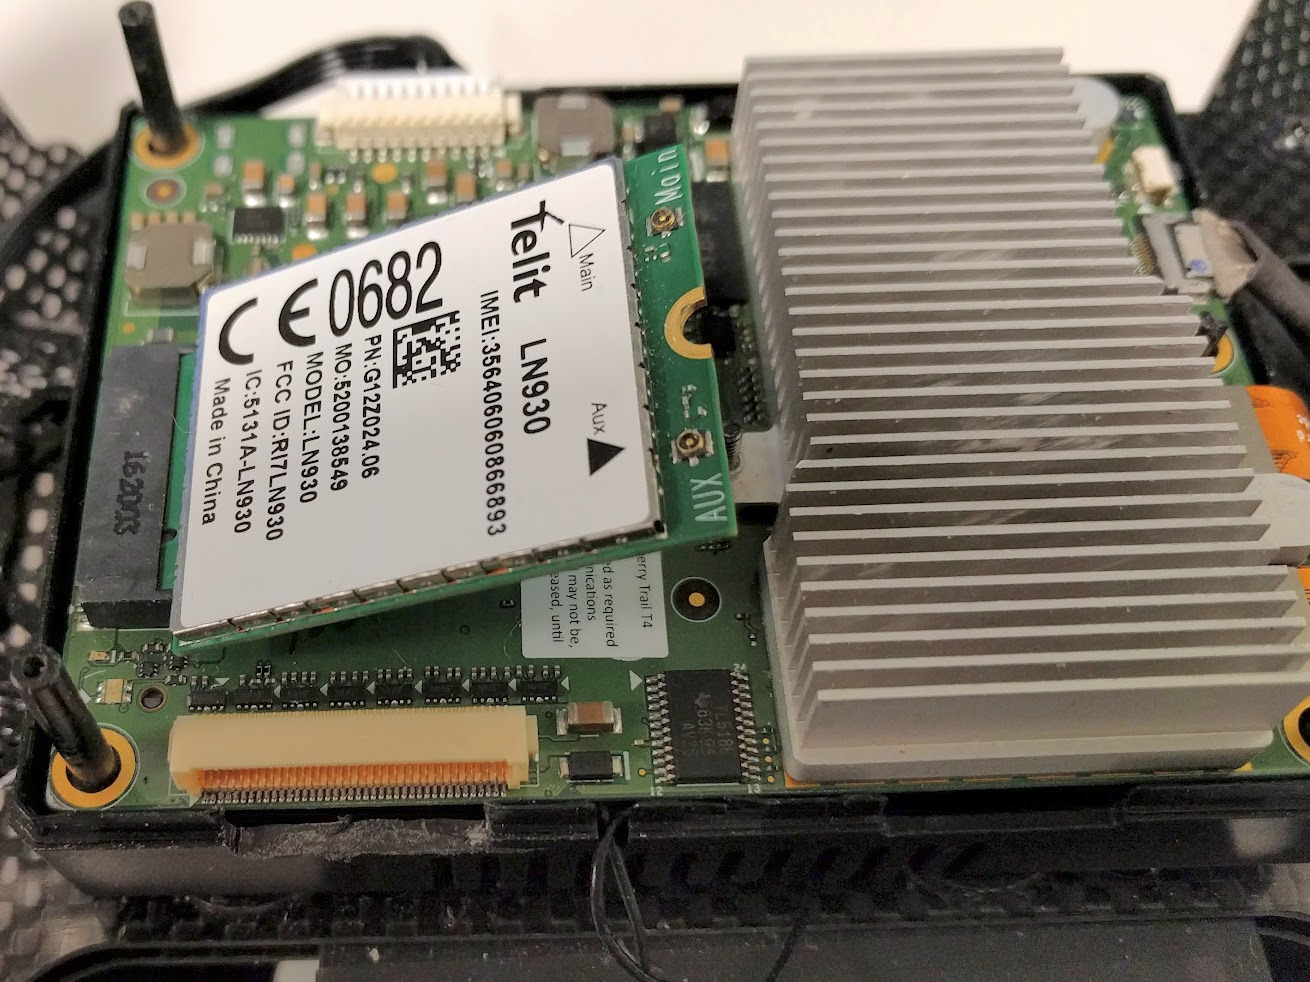
\includegraphics[width=\textwidth]{templates/images/chapter05/modem-insert-a.png} % first figure itself
        %\caption{first figure}
    \end{minipage}\hfill
    \begin{minipage}{0.48\textwidth}
        \centering
        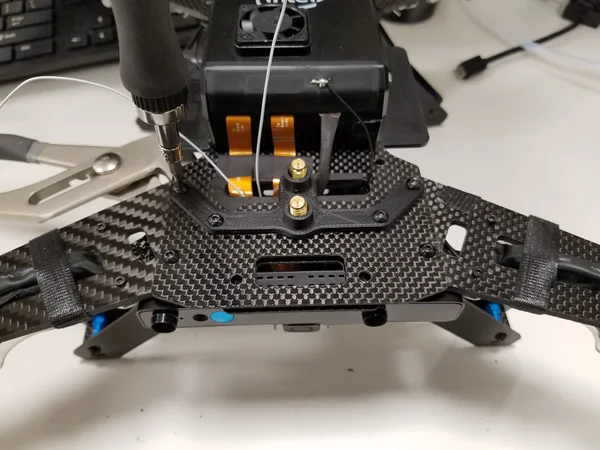
\includegraphics[width=\textwidth]{templates/images/chapter05/range-extender.png} % second figure itself
        %\caption{second figure}
    \end{minipage}
    \caption{Installing the modem and placing the additional antenna mounts.}
    \end{figure}

\section{Docker and Container Networking}

    There are many benefits for abstracting from a typical desktop OS installation in our specific use-case. A major one would be the compartmentalization of each of the processes that is to be run isolated from each other, as to ensure proper resource allocation, alleviating at the same time dependency problems previously mentioned. In this way, by updating only the docker runtime environment, each process can be install, updated and run independently. An added benefit of this setups would be of course its evolution to interact with the next-generation capabilities of 5G Core (or any next-gen network for that matter). By this, each initialized instance would be able to request a specific type of network slice according to its use, all the while providing added benefits of load balancing and fault tolerance that are eclipsed from regular OS or VM implementations.
    
    Following, are the three main docker container images that will be supplied with the finalized version of this drone platform, each geared towards a specific purpose in the overall use-case scenario.

    \subsection{srsue}
    
    srsLTE is a free and open-source LTE software suite developed by SRS %(www.softwareradiosystems.com). 
    The srsUE, srsENB and srsEPC applications include example configuration files that should be modified to meet the system configuration. Running the command \verb|sudo srsue| and by using the default configuration, creates a virtual network interface named "tun\_srsue" on the container with an IP in the network 172.16.0.x. Assuming the UE has been assigned an IP, we may now theoretically exchange traffic over the cellular link.
%https://github.com/srsLTE/srsLTE
    
    By default, containers are attached to a Docker network with a default route. This means everyone has internet access through the virtualized Docker network. In our use-case, the default-route parameter should be modified to point towards the \verb|srsue| container, which will handle the software stack that establishes the cellular connection either through a conventional modem or software-defined radio device. In order to make containers access the internet through the \verb|srsue| instead, we simply: 
    \begin{itemize}
    \item Configure network address translation at the UE
    \begin{lstlisting}
    docker exec virtual-srsepc iptables -t nat \
    -A POSTROUTING -s 172.16.0.0/24 -o eth0 -j MASQUERADE
    \end{lstlisting} This will masquerade all forwarded traffic from local containers (matched by source IP address) leaving the UE's eth0 (Docker) interface.
    
    \item Configure microservices containers to route traffic via the srsue by default

    \verb|docker exec virtual-srsue ip route replace default via 172.16.0.1|
    
    \end{itemize}
    Now we should have network access through the onboard UE software stack.
%[https://github.com/pgorczak/srslte-docker-emulated]
    
    Additionally, the library currently supports the Ettus Universal Hardware Driver (UHD) and the bladeRF driver. Thus, any hardware supported by UHD or bladeRF can be used, assuming allocation to the appropriate container. There is no sampling rate conversion, therefore the hardware should support 30.72 MHz clock in order to work correctly with LTE sampling frequencies and decode signals from live LTE base stations.
    
    %FDD and TDD configuration, Carrier Aggregation support, Cell search and synchronization procedure for the UE, Soft USIM supporting Milenage and XOR authentication, Hard USIM support using PCSC framework, Virtual network interface tun\_srsue created upon network attach
    %https://github.com/srsLTE/srsLTE

    \subsection{gstreamer}

    Due to poor streaming quality and performance by using conventional network feed streaming applications such as VLC, another solution would need to be implemented in order to further reduce the latency of the video transmission. For this reason, gstreamer, an open-source multimedia framework, is able to provide the granularity that's required in our use-case. Examples of that include -but are not limited- to enabling H.264 encoding, target frametime, resolution and aspect ratio, aswell as accepting multiple inputs at the same time. By configuring the appropriate default gateway setting on the networking parameters of this container and exposing its relevant network ports, we should be able to override using the system's bridge network and route the rtsp stream through \verb|srsue|.
    
%\newpage

    \subsection{mavlink-router}

    As previously mentioned, mavlink-router's sole purpose is to provide an encapsulation method for MAVLink packets to traverse the IP network. Additionally, its versatility in terms of addressing also provides a strategic advantage in terms of flexibility, as it can route streams to and from multiple devices independently at the same time. For this reason, by creating a basic container image and pointing the ttyS1 serial device to it, each running image will be able to handle separately traffic between the flight controller and ground station end points. Same as before, we can route the connectivity of the MAVLink messages through the software stack of \verb|srsue|.

%\newpage 

%The type of network a container uses, whether it is a bridge, an overlay, a macvlan network, or a custom network plugin, is transparent from within the container. From the container’s point of view, it has a network interface with an IP address, a gateway, a routing table, DNS services, and other networking details (assuming the container is not using the none network driver). This topic is about networking concerns from the point of view of the container. By default, when you create or run a container using docker create or docker run, it does not publish any of its ports to the outside world. To make a port available to services outside of Docker, or to Docker containers which are not connected to the container’s network, use the --publish or -p flag. This creates a firewall rule which maps a container port to a port on the Docker host to the outside world.

%    By default, the container is assigned an IP address for every Docker network it connects to. The IP address is assigned from the pool assigned to the network, so the Docker daemon effectively acts as a DHCP server for each container. Each network also has a default subnet mask and gateway. When the container starts, it can only be connected to a single network, using --network. However, you can connect a running container to multiple networks using docker network connect. When you start a container using the --network flag, you can specify the IP address assigned to the container on that network.
%https://docs.docker.com/config/containers/container-networking/
%    In terms of networking, a bridge network is a Link Layer device which forwards traffic between network segments. A bridge can be a hardware device or a software device running within a host machine’s kernel. In terms of Docker, a bridge network uses a software bridge which allows containers connected to the same bridge network to communicate, while providing isolation from containers which are not connected to that bridge network. The Docker bridge driver automatically installs rules in the host machine so that containers on different bridge networks cannot communicate directly with each other. Bridge networks apply to containers running on the same Docker daemon host. When you start Docker, a default bridge network (also called bridge) is created automatically, and newly-started containers connect to it unless otherwise specified. Containers on the default bridge network can only access each other by IP addresses, unless you use the --link option, which is considered legacy. All containers without a --network specified, are attached to the default bridge network. This can be a risk, as unrelated stacks/services/containers are then able to communicate. Using a user-defined network provides a scoped network in which only containers attached to that network are able to communicate by enterind the command \verb|$ docker network create my-net|.
%    You can specify the subnet, the IP address range, the gateway, and other options. When you create or remove a user-defined bridge or connect or disconnect a container from a user-defined bridge, Docker uses tools specific to the operating system to manage the underlying network infrastructure (such as adding or removing bridge devices or configuring iptables rules on Linux).
%https://docs.docker.com/network/bridge/ 

\chapter{Future Work and Development}
It should be apparent at this point that the drone platform described in detail in the previous chapters will be able to carry out the use-case demonstration it was intended for. During the development of this thesis, the use case scenario was validated to be fully operable through a wireless IP network, with acceptable delays in the video and control data transmission. What is also true is that there is plenty of room for improvements left in order to augment its capabilities and bring it closer to the next generation of interconnected aerial platforms of the future. Three key points have been selected to demonstrate some more or less obvious points for development - in the form of hardware or software - that would enhance the drone's capabilities and further improve its overall performance. 

\newpage
\section{Miniaturized Software Defined Radio platforms}

One area that the microelectronics industry has significantly influenced over the past half century is the digital communication systems sector, where microprocessor systems have been increasingly employed in the implementation of digital transceivers, yielding more versatile, powerful, and portable communication system platforms.

%An alternative to the superheterodyne architecture, which has reemerged as a potential solution in recent years, is the zero-IF architecture. A ZIF receiver utilizes a single frequency mixing stage with the local oscillator (LO) set directly to the frequency band of interest, translating the received signal down to baseband in phase (I) and quadrature (Q) signals. This architecture alleviates the stringent filtering requirements of the superheterodyne since all all analog filtering takes place at baseband, where filters are much easier to design and less expensive that custom RF/IF filters. The ADC and DAC are now operation in I/Q data at baseband, so the sample rate relative to the converted bandwidth can be reduced, saving significant power. Historically, the I/Q imbalance has limited the range of application that were appropriate for the ZIF architecture. This was due to two reasons: first, a discrete implementation of the ZIF architecture will suffer from mismatches both in the monolithic devices and also in the printed circuit board. In addition to this, the monolithic devices could pull from different fabrication lots, making exact matching very difficult due to native process variation. A discrete implementation will also have the processor physically separated from the RF components, making a quadrature correction algorithm very difficult to implement across frequency, temperature and bandwidth. Moore's law or integration of the ZIF architecture into a monolithic transceiver device provides the path forward for next-generation systems. By having the analog and RF signal chain on a single piece of silicon, process variation will be kept to a minimum. Digital signal processing blocks can be incorporated into the transceiver, removing the boundary between the quadrature calibration algorithm and the signal chain. This approach provides both unparalleled improvements and can also match the superheterodyne architecture for performance specifications. 

\begin{figure}[H]
    \centering
    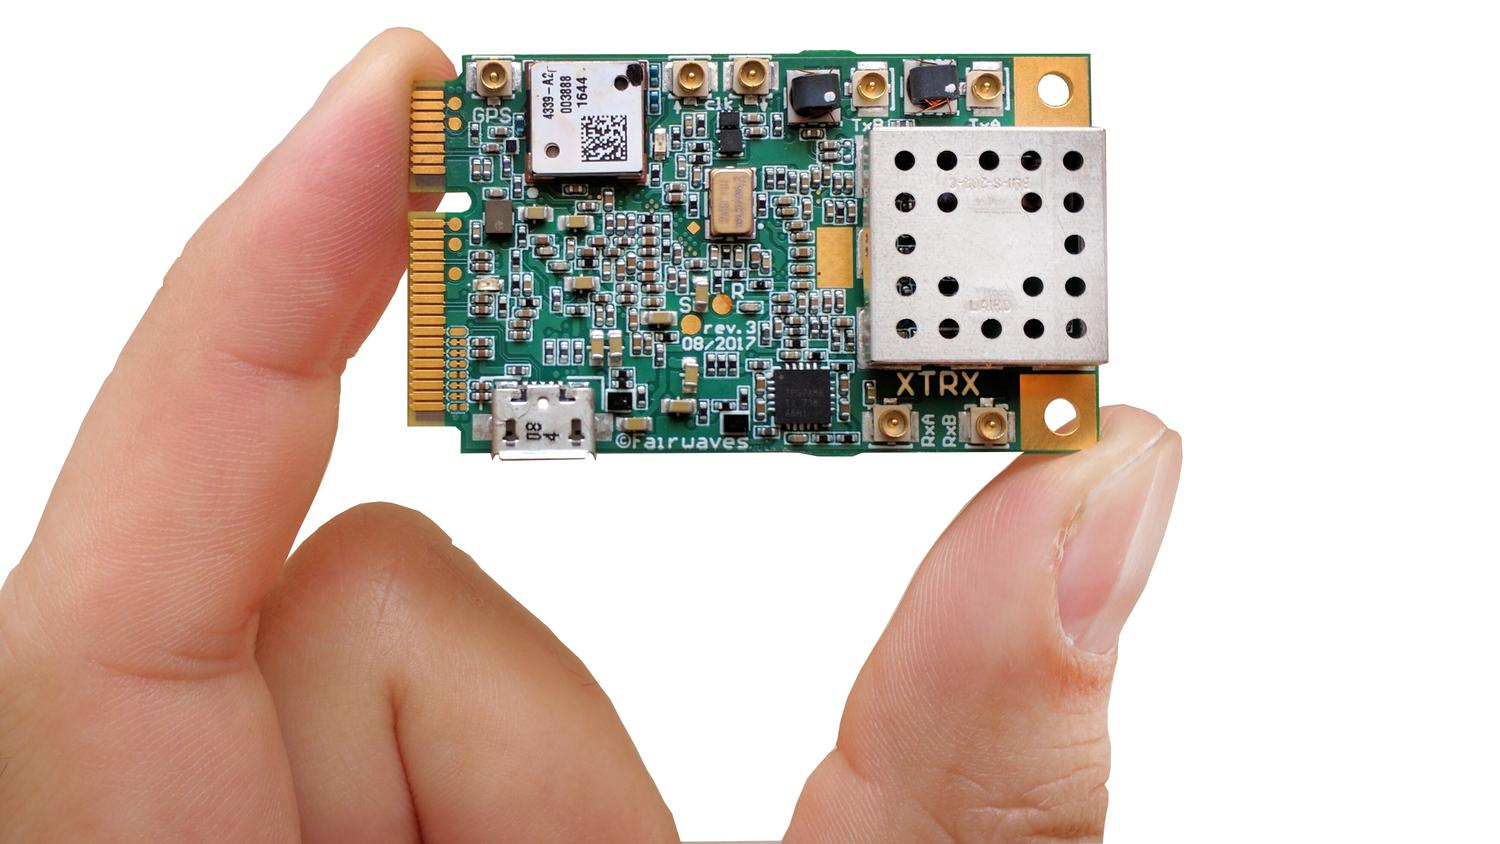
\includegraphics[width=0.9\textwidth]{templates/images/chapter06/xtrx-hand.jpg}
    \caption{XTRX Pro Board for Scale. Source: \cite{xtrx-io}}
    \label{fig:xtrx-io}
\end{figure}

Devices like the XTRX SDR shown in Figure \ref{fig:xtrx-io} integrate the full RF, analog and digital signal chain onto a single CMOS device. Devices like the LMS7002M focus on very low power consumption small form factor SDR applications such as UAV data links and handheld communication systems. This opens up a new design potential for a different suite of applications where using wideband waveforms or occupying noncontiguous spectrum can now be implemented in a much smaller form factor. The XTRX offers a 2x2 MIMO configuration with a stable clock accurate enough for cellular standards, an onboard GPS disciplined oscillator (GPSDO) and a SIM card reader. When inserted into an appropriate Mini PCIe slot, it appears as a USB SIM card reader, able to interface with a wide variety of single board computers such as the one used in our usecase.

\newpage
\section{Leveraging new streaming protocols}

%\begin{figure}[H]
%    \centering
%    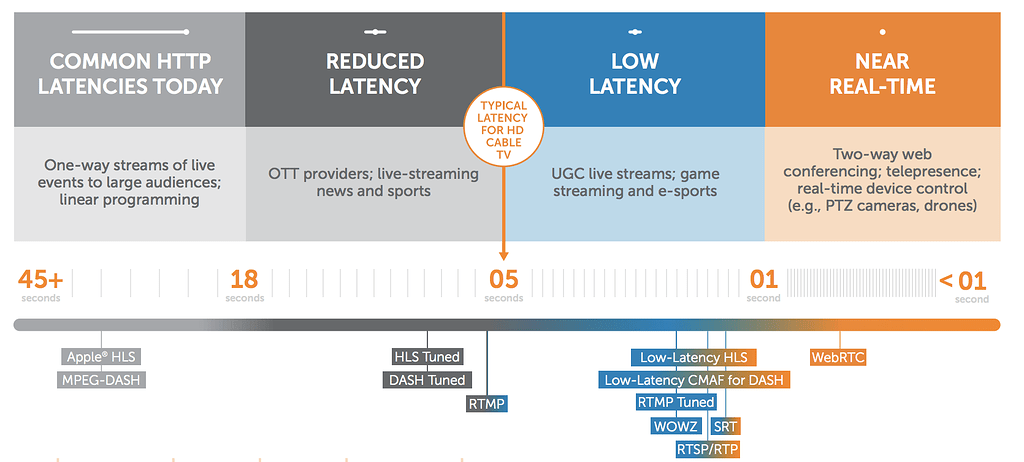
\includegraphics[width=\textwidth]{templates/images/chapter06/latency-comparison.png}
%    \caption{. Source: [*]}
%    \label{fig:board-diagram}
%\end{figure}
%https://www.wowza.com/blog/streaming-protocols

Traditional streaming protocols, such as RTSP and RTMP, support low-latency streaming. But they aren’t supported on all endpoints and work best for streaming to a small audience from a dedicated media server. These protocols achieve this by transmitting the data using a firehose approach rather than requiring local caching.

WebRTC is a combination of standards, protocols, and JavaScript APIs created by the World Wide Web Consortium (W3C) that enables real-time communications, allowing browser applications to make calls without any plugins and designed primarily with latency in mind. Different bodies such as the Internet Engineering Task Force, created to standardize the used protocols with browser APIs have been working on this implementation. Users connecting via Chrome, Firefox, or Safari can communicate directly through their browsers — enabling sub-500 millisecond latency to more than 85\% of all installed browsers globally for real-time communications on the internet.

\begin{table}[!ht]
           \begin{threeparttable}
        \caption{Comparison Between Video Streaming Protocols in ms. Source: \cite{impl-analysis-rtsp}}
        \label{tab:video-stream-protocols}
        \setlength\tabcolsep{1pt} % make LaTeX figure out intercolumn spacing
        
        \begin{tabular*}{\columnwidth}{@{\extracolsep{\fill}} lllll}
        \toprule
              &Establishment  &Reception  &Client to Client&Client to Web\\
        %     \multicolumn{4}{c}{Accuracy (\%)} \\ 
        %\cmidrule{3-6}
        %     & & K3 & K6 & L1 & mean\tnote{c} \\
        \midrule
              \textbf{RTSP} &2304 ms & 2161 ms & 37.807 ms & -\\
        \addlinespace
             \textbf{WebRTC} &1835 ms &1709ms&8.072 ms & 5.112 ms \\
        \addlinespace
              \textbf{Skype} &-&-&-&11.646 ms\\
        \bottomrule
        \end{tabular*}
        
        \smallskip
        \scriptsize
           \end{threeparttable}
        \end{table}

In a relevant work \cite{impl-analysis-rtsp}, two video streaming platforms implementing the most commonly used video streaming protocols, RTSP and WebRTC, have been implemented in order to conclude which offers the best results in the scope of web real-time video streaming applications. The analysis includes different parameters, namely the connection establishment and stream reception time, critical factors in applications such as our usecase. The results of the experiments discussed suggest that the use of the WebRTC protocol offers a vastly improved performance over the others, as can be seen in Table \ref{fig:board-diagram}.

%The performance improvement of the WebRTC implementation with respect to the RTSP implementation could be related to the use of UDP in all communications by the WebRTC protocol, whereas, in the RTSP protocol, TCP is used for the control. On the other hand, RTSP does not drop video packets, while the WebRTC protocol can do it if necessary. Finally, for peer-to-peer communications, WebRTC sends the video directly to the other peer, while, in the case of RTSP, the video is sent to the server and the server sends it to the other peer. Moreover, the WebRTC streaming platform shows better results than the analysed streaming applications in the stream reception time and in the stream establishment time in all cases, which means that, taking these measurements into account, the implemented streaming platform offers a better QoS than the studied applications. From the experiments, it is concluded that significant improvements have been obtained in WebRTC over RTSP for both communication establishment time and package sending time. Moreover, the implemented systems have been compared with the most common commercial applications through two experiments. Therefore, at this point, it is possible to confirm that the use of the WebRTC protocol provides better QoE and QoS than other protocols, and that the implemented Direct WebRTC system offers good results, according to the performed experiments.

\newpage
\section{Going cloud native}

Cloud-native today is almost synonymous with containers orchestrated by Kubernetes.  It wasn’t always thus.  It’s perfectly possible to build something that is cloud-native in all respects other than running in containers – i.e. dynamically orchestratable stateless microservices running in VMs – and production deployments have demonstrated many of the benefits, particularly with regard to simple, rapid scaling of the system and the automation of lifecycle management operations such as software upgrades.  

%Originally released by Google as recently as July 2015, Kubernetes became the seed project of the Cloud Native Computing Foundation (CNCF), and rapidly eclipsed all the other container orchestration solutions that were out there at the time.  It is now available in multiple mature distros including Red Hat OpenShift and Pivotal Container Services, and is also offered as a service by all the major public cloud operators.  It’s the only game in town when it comes to deploying and managing cloud native applications.  And, for the first time, we have a genuinely common platform for running cloud applications across both private and public clouds.  This is hugely helpful to telcos who are starting to explore the possibility of hybrid clouds for NFV.

Drawing a parallelism to the ETSI NFV architecture, it essentially covers the Virtual Infrastructure Manager (VIM) and VNF Manager (VNFM) roles. In its VIM role, Kubernetes schedules container-based workloads and manages their network connectivity, including a kind of Load Balancer as a Service, making it easy to deploy scale-out microservices. In its VNFM role, Kubernetes can monitor the health of each container instance and restart any failed instance.  It can also monitor the relative load on a set of container instances that are providing some specific micro-service and can scale out (or scale in) by spinning up new containers or spinning down existing ones.  In this sense, Kubernetes acts as a Generic VNFM.  For some types of workloads, especially stateful ones such as databases or state stores, Kubernetes native functionality for lifecycle management is not sufficient. In NFV terms, it comprizes a standardized way of building Specific VNFMs. But the beauty of Kubernetes is that it can provide a common environment across all types of cloud infrastructures. In this way, Kubernetes allows us to achieve a unified strategy for NFV that is entirely compelling.

%    \begin{figure}[H]
%        \centering
%        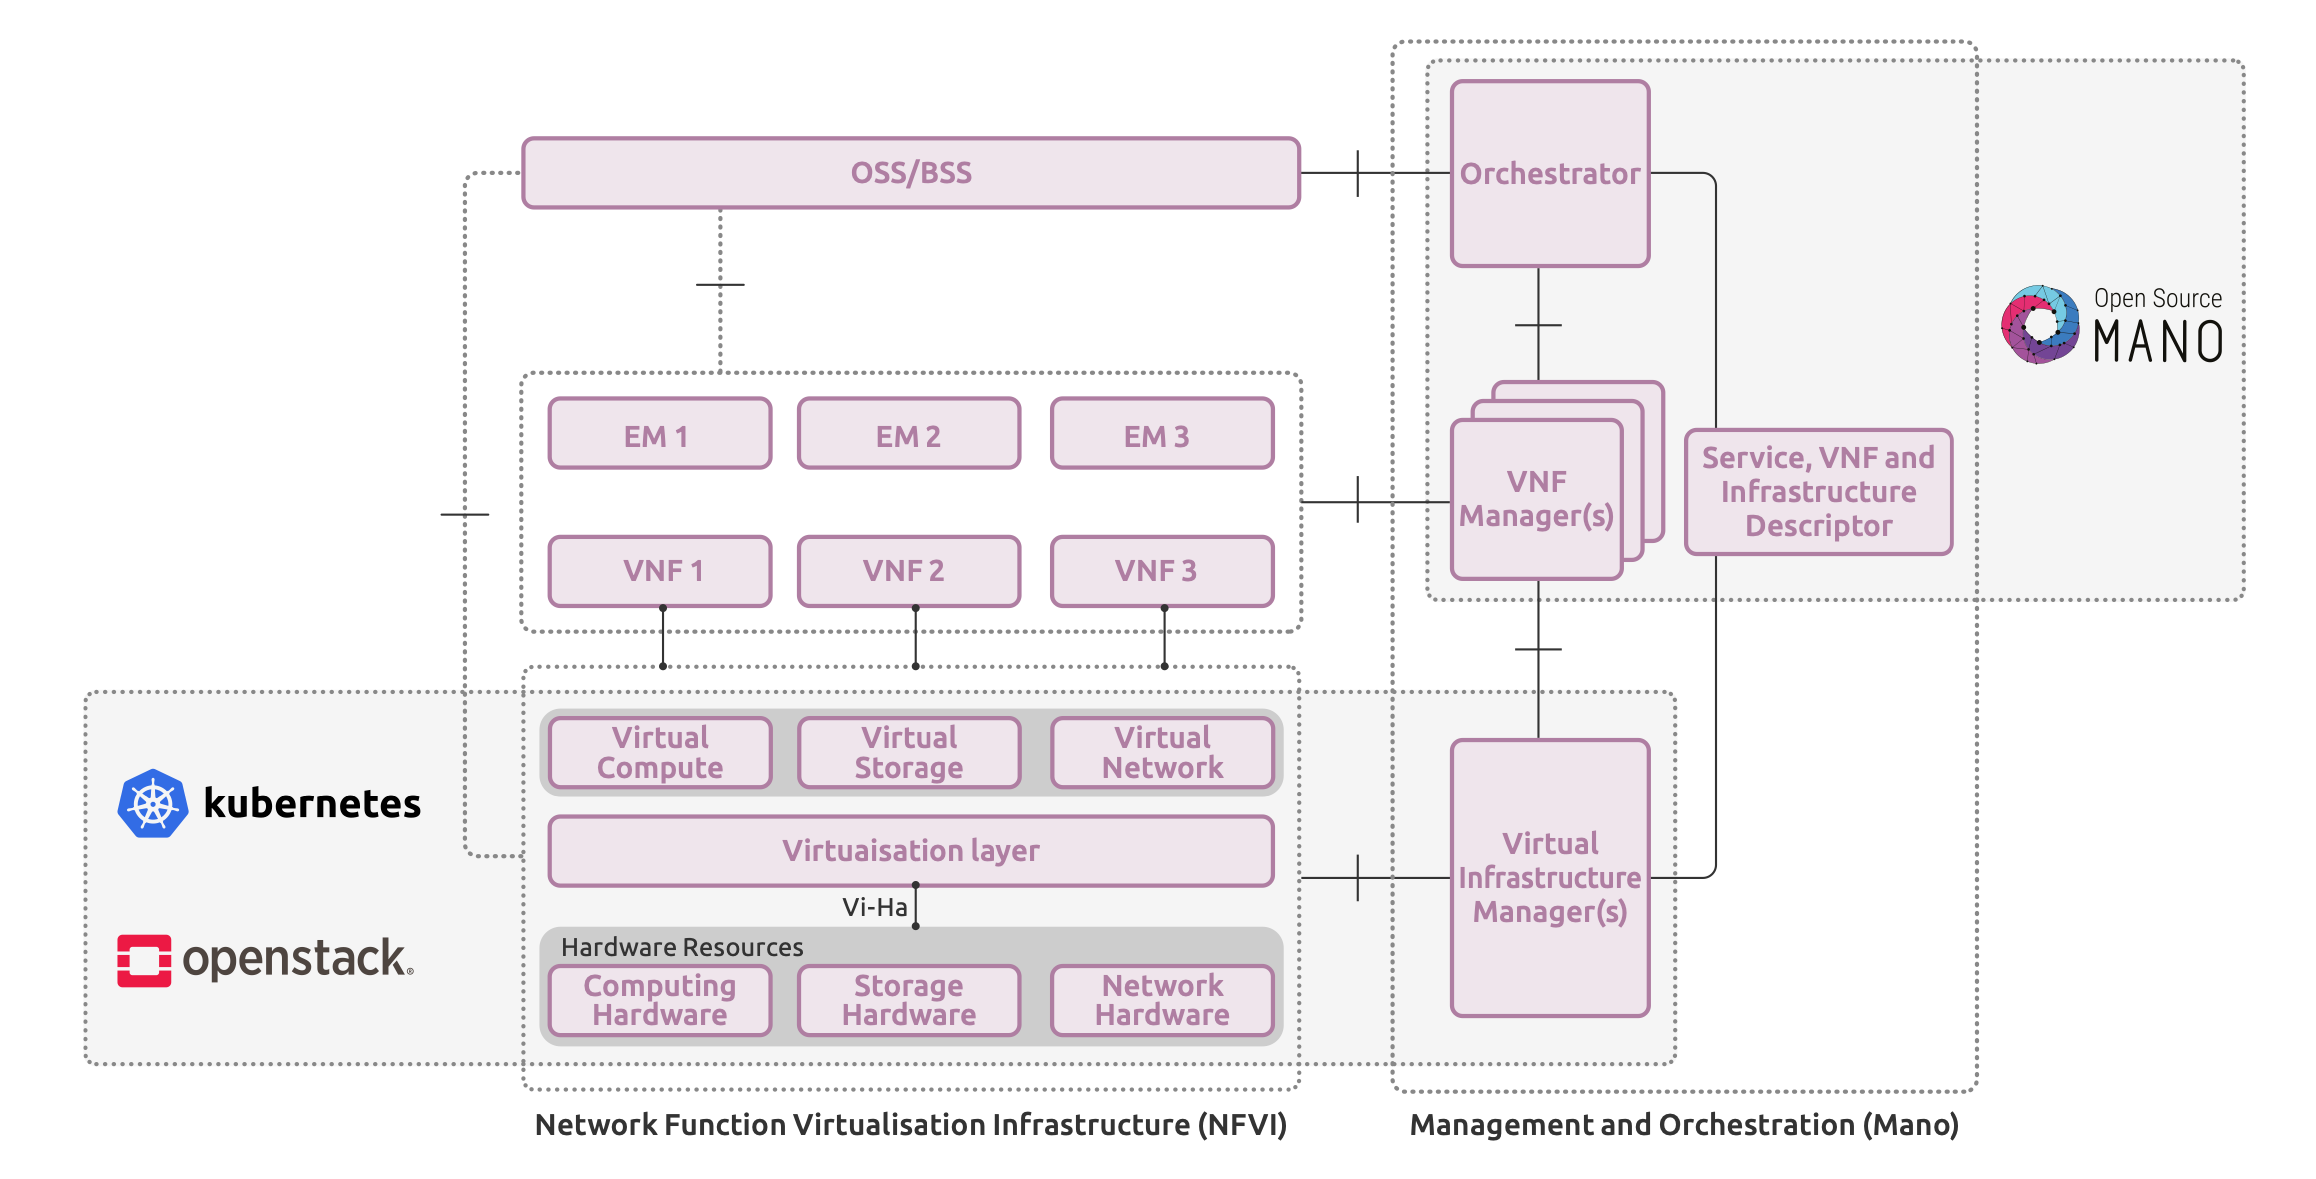
\includegraphics[width=0.9\textwidth]{templates/images/chapter06/kubernetes.png}
%        \caption{. Source: [*]}
%        \label{fig:board-diagram}
%    \end{figure}

%But Kubernetes goes way beyond the simple application lifecycle management envisaged by the ETSI NFV effort.  Kubernetes itself, together with a growing ecosystem of open source projects that surround it, is at the heart of a movement towards a declarative, version-controlled approach to defining both software infrastructure and applications.  The vision here is for all aspects of a complex cloud native system, including cluster infrastructure and application configuration, to be described in a set of documents that are under version control, typically in a Git repository, which maintains a complete history of every change.  These documents describe the desired state of the system, and a set of software agents act so as to ensure that the actual state of the system is automatically aligned with the desired state.  With the aid of a service mesh, changes to system configuration or software version can be automatically “canary” tested on a small proportion of traffic prior to be rolled out fully across the deployment.  If any issues are detected, the change can simply be rolled back. The high degree of automation and control offered by this kind of approach has enabled Web-scale companies to reduce software release cycles from months to minutes.

%This means today’s NFV infrastructure needs to be built on a hypervisor-based virtualization environment supporting VNFs deployed as virtual machines, with OpenStack acting as the VIM.  The conventional wisdom seems to be that you run Kubernetes on top of your existing VIM  and this is certainly possible: you just provision a number of VMs and treat these as hosts for the purposes of installing a Kubernetes cluster.  But then you end up with a two-tier environment in which you have to deploy and orchestrate services across some mix of cloud native network functions in containers and VM-based VNFs, where orchestration is driving some mix of Kubernetes, OpenStack or VMware APIs and where Kubernetes needs to coexist with proprietary VNFMs for life-cycle management. In our work with cloud-native VNFs, containers and Kubernetes, we’ve seen just how much easier it is to deploy and manage large scale applications using this approach compared with traditional hypervisor-based approaches.  The difference is huge.  We firmly believe that adopting this approach is the key to unlocking the massive potential of NFV to simplify operations and accelerate the pace of innovation in services. We think network operators should ratchet up the pressure on their vendors to deliver genuinely cloud native, container-based VNFs, and get serious about Kubernetes as an integral part of their NFV infrastructure.  Without any question, that is where the future lies.
%[https://www.metaswitch.com/blog/the-future-of-nfvi-is-kubernetes]

%\section{Closing Words}
%In October 2012, when a group of 13 network operators launched their white paper describing Network Functions Virtualization, the world of cloud computing technology looked very different than it does today.  As cloud computing has evolved, and as telcos have developed a deeper understanding of it, so the vision for NFV has evolved and changed out of all recognition. The early vision of NFV focused on moving away from proprietary hardware to software running on commercial off-the-shelf servers.  This was described in terms of “software appliances” and in describing the compute environment in which those would run, the NFV pioneers took their inspiration from enterprise IT practices of that era, which focused on consolidating servers with the aid of hypervisors that essentially virtualized the physical host environment.

%Meanwhile, hyperscale Web players were developing cloud-based system architectures that supported massive scalability with a high degree of resilience, which can be evolved very rapidly through incremental software enhancements, and can be operated very cost-effectively with the aid of a high degree of operations automation.  The set of practices developed by these players has come to be known as “cloud-native”, which can be summarized as dynamically orchestratable micro-services architectures, often based on stateless processing elements working with separate state storage micro-services, all deployed in Linux containers.

%It’s been clear to most network operators for at least a couple of years that cloud-native, microservices-based architectures is the right way to do NFV, for the following reasons:
%\begin{itemize}

%\item Promote rapid evolution of software capabilities to enable enhancement of services and operations, unlike legacy monolithic software architectures with their monthly upgrade cycles and their costly and complicated roll-out procedures.
%\item Enable independent and dynamic scaling of different functional elements of the system with active-active N+k redundancy, which minimizes the hardware resources required to deliver any given service.
%\item Software packaged in containers is inherently more portable than VMs and does much to eliminate the problem of complex dependencies between VMs and the underlying infrastructure which has been a major issue for NFV deployments to date.
%\item The cloud-native ecosystem includes some outstandingly useful open source projects. All of these combine to simplify, accelerate and lower the cost of developing, deploying and operating cloud-native network functions.
%\end{itemize}

%5G is the first new generation of mobile technology since the advent of the NFV era, and as such it represents a great opportunity to do NFV right – that is, the cloud-native way.  The 3GPP standards for 5G are designed to promote a cloud-native approach to the 5G core – but they don’t actually guarantee that 5G core products will be recognisably cloud-native.

%\appendix
%\chapter{Tables}

\begin{table}
\caption{Armadillos}
\label{arm:table}
\begin{center}
\begin{tabular}{||l|l||}\hline
Armadillos & are \\\hline
our	   & friends \\\hline
\end{tabular}
\end{center}
\end{table}

%-------------------------------------------------------------------------------------------------------------------------------------------------------%

\begin{sidewaystable*}
\scriptsize
 \caption{Ettus Research Software Defined Radio Platforms}

\label{my-label}
\begin{tabularx}{\textwidth}{@{}l*{10}{C}c@{}}
\addlinespace
\addlinespace
\toprule
     & Frequency Range(MHz) & Channel BW(MHz) & Rx/Tx & Duplex (Full/Half) & Transmit  (dBm) & Sample  (MSps) & Interface & Chipset (FPGA) &  Gates (k) & Size (mm)  & Price  \\ 
     \addlinespace
\midrule
\addlinespace 
USRP B200 & 70-6000 & 56 & 1/1 & Full & 10 & 61,44 & USB3.0 & XC6SLX75 & Gates & Vendor & USD / EUR  \\

USRP B200mini-i & 70-6000 & 56 & 1/1 & Full & 10 & 61,44 & USBOTG & XC6SLX75 & Gates & Vendor & USD / EUR  \\ 

USRP B205mini-i & 70-6000 & 56 & 1/1 & Full & 10 & 61,44 & USBOTG & XC6SLX150 & Gates & Vendor & USD / EUR  \\ 

USRP B200mini & 70-6000 & 56 & 1/1 & Full & 10 & 61,44 & USBOTG & XC6SLX75 & Gates & Vendor & USD / EUR  \\  

USRP B210   & 70-6000 & 56/30.72 & 2/2 & Full/Half & 10 & 61,44 & USB3.0 & XC6SLX150 & 100 & Ettus R.    & 1119 \$ /  \\ 

\addlinespace

USRP E310 & 70-6000 & 56 & 2/2 & Full & 10 & 10 & 1x1Gb & Zynq7020 & Gates & Vendor & USD / EUR  \\ 

USRP E312 & 70-6000 & 56 & 2/2 & Full & 10 & 10 & 1x1Gb & Zynq7020 & Gates & Vendor & USD / EUR  \\ 

USRP E313 & 70-6000 & 56 & 2/2 & Full & 10 & 10 & 1x1Gb & Zynq7020 & Gates & Vendor & USD / EUR  \\ 

\addlinespace 

USRP N200 & - & - & - & - & 15 & 100 & 1x1Gb & DSP1800 & Gates & Vendor & USD / EUR  \\  

USRP N210 & - & - & - & - & 15 & 100 & 1x1Gb & DSP3400 & Gates & Vendor & USD / EUR  \\  

USRP N300 & 10-6000 & 100 & 2/2 & Full & 20 & 153.6 & 2xSFP+ & Zynq7035 & Gates & Vendor & USD / EUR  \\ 

USRP N310 & 10-6000 & 100 & 4/4 & Full & 20 & 153.6 & 2xSFP+ & Zynq7100 & Gates & Vendor & USD / EUR  \\ 

\addlinespace 

USRP X300 & - & - & - & - & 10 & 200 & 2x10Gb & XC7K325T & - & Vendor & USD / EUR  \\  

USRP X310 & - & - & - & - & 10 & 200 & 2x10Gb & XC7K410T & - & Vendor & USD / EUR  \\  

\addlinespace 
\midrule
\addlinespace 

CBX 782760 & range & BW & Rx/Tx & Duplex & - & - & - & - & - & - & USD / EUR  \\ 
CBX 783353 & range & BW & Rx/Tx & Duplex & - & - & - & - & - & - & USD / EUR  \\
\addlinespace  
SBX 782761 & range & BW & Rx/Tx & Duplex & - & - & - & - & - & - & USD / EUR  \\  
SBX 783351 & range & BW & Rx/Tx & Duplex & - & - & - & - & - & - & USD / EUR  \\  
\addlinespace 
TwinRX & range & BW & Rx/Tx & Duplex & - & - & - & - & - & - & USD / EUR  \\ 
\addlinespace 
UBX 783775-01 & range & BW & Rx/Tx & Duplex & - & - & - & - & - & - & USD / EUR  \\  
UBX 783774-01 & range & BW & Rx/Tx & Duplex & - & - & - & - & - & - & USD / EUR  \\ 
\addlinespace  
WBX 782759 & range & BW & Rx/Tx & Duplex & - & - & - & - & - & - & USD / EUR  \\  
WBX 783352 & range & BW & Rx/Tx & Duplex & - & - & - & - & - & - & USD / EUR  \\  

\addlinespace 
\midrule
\end{tabularx}
\end{sidewaystable*}

%-------------------------------------------------------------------------------------------------------------------------------------------------------%

\begin{table} \centering
    \begin{tabular}{@{} cl*{12}c @{}}
        &&&& \multicolumn{10}{c}{Software Defined Radio Platforms} \\[2ex]
        && \rot{Open Source} && \rot{Integration} & \rot{Scope} & \rot{Time} & \rot{Cost} 
        & \rot{Quality} & \rot{Human Resource} & \rot{Communication} 
        & \rot{Risk} & \rot{Procurement} & \rot{\shortstack[l]{Stakeholder\\Management}} \\
        \cmidrule{2-13}
        & GNU Radio 	& \OK && \OK & \OK & \OK & \OK & \OK & \OK & \OK & \OK & \OK & \OK \\
        & C++ API  	& \OK && \OK & \OK & \OK & \OK & \OK & \OK & \OK & \OK & \OK & \OK \\
        & Python API   	& \OK && \OK & \OK & \OK & \OK & \OK & \OK & \OK & \OK & \OK & \OK \\
        & Matlab Simulink   & \OK && \OK & \OK & \OK & \OK & \OK & \OK & \OK & \OK & \OK & \OK \\
        \cmidrule{2-13}
        & Amarisoft LTE	& \OK && \OK & \OK & \OK & \OK & \OK & \OK & \OK & \OK & \OK & \OK \\
        & Open BTS		& \OK && \OK & \OK & \OK & \OK & \OK & \OK & \OK & \OK & \OK & \OK \\
        & Osmocom  		& \OK && \OK & \OK & \OK & \OK & \OK & \OK & \OK & \OK & \OK & \OK \\
        & GNURadio 		& \OK && \OK & \OK & \OK & \OK & \OK & \OK & \OK & \OK & \OK & \OK \\
        & GNURadio	  	& \OK && \OK & \OK & \OK & \OK & \OK & \OK & \OK & \OK & \OK & \OK \\
 %\rot{\rlap{~Software}}
        & Closing		& \OK &   &   &   &   &   & \OK &   & \OK & \OK \\
        \cmidrule[1pt]{2-13}
    \end{tabular}
    \caption{Some caption}
\end{table}

%-------------------------------------------------------------------------------------------------------------------------------------------------------%


\clearpage
\newpage

%\include{appb}
%\printglossary[type=\acronymtype]
\printnoidxglossary[type=\acronymtype]

%% This defines the bibliography file (main.bib) and the bibliography style.
%% If you want to create a bibliography file by hand, change the contents of
%% this file to a `thebibliography' environment.  For more information 
%% see section 4.3 of the LaTeX manual.
\begin{singlespace}
\bibliography{main}
\bibliographystyle{IEEEtran}
\end{singlespace}

\end{document}